% This is the Reed College LaTeX thesis template. Most of the work
% for the document class was done by Sam Noble (SN), as well as this
% template. Later comments etc. by Ben Salzberg (BTS). Additional
% restructuring and APA support by Jess Youngberg (JY).
% Your comments and suggestions are more than welcome; please email
% them to cus@reed.edu
%
% See http://web.reed.edu/cis/help/latex.html for help. There are a
% great bunch of help pages there, with notes on
% getting started, bibtex, etc. Go there and read it if you're not
% already familiar with LaTeX.
%
% Any line that starts with a percent symbol is a comment.
% They won't show up in the document, and are useful for notes
% to yourself and explaining commands.
% Commenting also removes a line from the document;
% very handy for troubleshooting problems. -BTS

% As far as I know, this follows the requirements laid out in
% the 2002-2003 Senior Handbook. Ask a librarian to check the
% document before binding. -SN

%%
%% Preamble
%%
% \documentclass{<something>} must begin each LaTeX document
\documentclass[11pt,twoside]{reedthesis}
\usepackage[paperheight=237mm,paperwidth=168mm,bottom=20mm, top=20mm, outer=1.5cm, inner=2.4cm]{geometry}
% Packages are extensions to the basic LaTeX functions. Whatever you
% want to typeset, there is probably a package out there for it.
% Chemistry (chemtex), screenplays, you name it.
% Check out CTAN to see: http://www.ctan.org/
%%
\usepackage{graphicx,latexsym}
\usepackage{amsmath}
\usepackage{amssymb,amsthm}
\usepackage{longtable,booktabs,setspace}
\usepackage{chemarr} %% Useful for one reaction arrow, useless if you're not a chem major
\usepackage[hyphens]{url}
% Added by CII
\usepackage{hyperref}
\usepackage{lmodern}
\usepackage{float}
\floatplacement{figure}{H}
% End of CII addition
\usepackage{rotating}

% Next line commented out by CII
%%% \usepackage{natbib}
% Comment out the natbib line above and uncomment the following two lines to use the new
% biblatex-chicago style, for Chicago A. Also make some changes at the end where the
% bibliography is included.
%\usepackage{biblatex-chicago}
%\bibliography{thesis}


% Added by CII (Thanks, Hadley!)
% Use ref for internal links
\renewcommand{\hyperref}[2][???]{\autoref{#1}}
\def\chapterautorefname{Chapter}
\def\sectionautorefname{Section}
\def\subsectionautorefname{Subsection}
% End of CII addition

% Added by CII
\usepackage{caption}
\captionsetup{width=5in}
% End of CII addition

% \usepackage{times} % other fonts are available like times, bookman, charter, palatino

% Syntax highlighting #22

% To pass between YAML and LaTeX the dollar signs are added by CII
\title{Plant Species Climatic Niche and its Relationship with Population
Responses to Extreme Drought}
\author{María Ángeles Pérez Navarro}
% The month and year that you submit your FINAL draft TO THE LIBRARY (May or December)
\date{Dec 2019}
\degree{DOCTORADO EN ECOLOGIA TERRESTRE}
% \division{}
\advisor{Prof.~Francisco Lloret Maya}
\institution{Autonomous University of Barcelona}
% \degree{DOCTORADO EN ECOLOGIA TERRESTRE}
%If you have two advisors for some reason, you can use the following
% Uncommented out by CII
\altadvisor{Prof.~Miguel Ángel Esteve Selma}
% End of CII addition

%%% Remember to use the correct department!
\department{Centre de Recerca Ecològica i Aplicacions Forestals}
% if you're writing a thesis in an interdisciplinary major,
% uncomment the line below and change the text as appropriate.
% check the Senior Handbook if unsure.
%\thedivisionof{The Established Interdisciplinary Committee for}
% if you want the approval page to say "Approved for the Committee",
% uncomment the next line
%\approvedforthe{Committee}

% Added by CII
%%% Copied from knitr
%% maxwidth is the original width if it's less than linewidth
%% otherwise use linewidth (to make sure the graphics do not exceed the margin)
\makeatletter
\def\maxwidth{ %
  \ifdim\Gin@nat@width>\linewidth
    \linewidth
  \else
    \Gin@nat@width
  \fi
}
\makeatother

\renewcommand{\contentsname}{Table of Contents}
% End of CII addition

\setlength{\parskip}{0pt}

% Added by CII

\providecommand{\tightlist}{%
  \setlength{\itemsep}{0pt}\setlength{\parskip}{0pt}}

\Acknowledgements{
\setlength{\parindent}{30pt} A pesar de ser firme defensora de que la
tesis no supone un mérito excepcional digno de especiales
reconocimientos, no desperdiciaré la oportunidad de agradecer todo lo
vivido durante estos años y dejar grabado lo mucho que deben estas
páginas a las personas que me rodean.\par
Durante esta etapa, que empezó cuando llegué a Barcelona, he tenido la
suerte de encontrar a personas maravillosas, de viajar por el mundo y de
aprender sobre diferentes aspectos de la vida. Quiero agradecer en
primer lugar, a la que fue mi primera familia en Catalunya, mis
compañeros de máster, en especial a Estrella, Aida, Alba, Aina, Carla,
Enrique, John y Gustavo y a mis compañeros de piso Laura y Josan.
Gracias por los ratos en el césped, las visitas a Mataró y las noches
arreglando el mundo en el \emph{Cop de ma}, gracias, en definitiva, por
hacerme sentir en casa.\par
Cuando una empieza la tesis le dicen que debería preocuparse de escoger
bien a sus directores porque son personas con las que tendrá que
compartir cuatro años y ver más a menudo que a sus propios padres. Yo
con Paco apenas tuve dos reuniones antes de solicitar el doctorado.
Después de estos más de cuatro años trabajando juntos sé que si volviese
atrás volvería a elegirte. Gracias Paco por el ejemplo, por las charlas
en los viajes, por tu forma de pensar tan crítica, transversal y
profunda, por enseñarme tanto más allá de lo estrictamente
académico\ldots{} A Miguel Ángel lo conocía más. Fui su alumna durante
la carrera y sé que pocas personas tienen un conocimiento más holístico
de la naturaleza murciana, mayor integridad y devoción por su trabajo.
Gracias por tu visión naturalista y aplicada, gracias por las charlas de
política y las explicaciones sobre el Mar Menor. Durante estos años he
crecido con y gracias a vosotros, y no podría sentirme más
afortunada.\par
Además esta tesis no hubiese tenido los mismos resultados sino hubiese
compartido las dudas, preocupaciones, alegrías y el desánimo con tantos
buenos compañeros. Gracias a los compañeros de despacho, a Anna, Javi,
Judit, Carlos, Manu, Marta, Pere y Pol. Sin duda las penas han sido
menos penas con vosotros y las fiestas, almuerzos y barbacoas mucho más
divertidas. Gracias por las risas y la terapia de grupo. No me
acostumbro a pensar en un trabajo sin vosotros.\par
Gracias también a los compañeros de grupo. Enric, Jordi, Luciana y
Nuria, el \emph{phoskitos lab} no podría tener mejor plantilla. Con
vosotros se demuestra que hacer ciencia no está reñido con un ambiente
laboral de calidad, colaborativo, respetuoso y divertido. Gracias por
tantos buenos momentos, por las discusiones académicas y las no tan
académicas, por las salidas a la montaña y las jornadas de convivencia
en los congresos. Quiero agradecer también a mis compañeros de
departamento en Murcia. Gracias a Paqui, Juan Miguel y Pablo por el
trabajo de campo y de despacho, por estar siempre ahí pese a la
distancia, por no haber dudado en ayudar siempre que lo he necesitado.
Gracias también a Guillem por las semanas de trabajo y convivencia en
Murcia y tus dosis de amabilidad y optimismo, a Pep Serra y Gerard Sapes
por los sabios consejos y la inspiración.\par
Durante estos últimos años también he tenido la oportunidad de librarme
de los calurosos veranos catalanes y murcianos escapándome de estancia a
otros países. Gracias a Jens-Christian por la acogida en Aarhus y a
Antoine y Olivier por la estancia en Suiza. Me quedo con el recuerdo de
los paseos en bici por Dinamarca y la estampa de los Alpes por la
ventana del despacho y las barbacoas en el lago Leman. Gracias también a
los que han estado siempre ahí, a los amigos de toda la vida, Jose,
Maria José, Mari Nieves, Maria Victoria, Álvaro Talavera y Pedro.
Gracias por estar tan cerca a pesar de los kilómetros, gracias por las
visitas, por aguantar con paciencia mis quejas sobre política y ciencia,
por los cafés, las terapias y el consuelo. Gracias también a Victor
Valero por el tiempo que hemos pasado juntos en Barcelona, por las horas
de desahogo mutuo y los planes culturales.\par
Quiero agradecer también a mi familia. A mis tios, por ayudarme siempre
que les ha sido posible. A mi hermano mayor, por plantar en mi la
semilla del amor por la naturaleza, sin tu ejemplo no hubiese dado los
primeros pasos del camino que ahora completo. Gracias también a mi
hermano mellizo por la ayuda incondicional e implicación, llegando
incluso a armarte con botas y cinta métrica para echar una mano en el
trabajo de campo.\par
Gracias sobre todo a quien desde hace más de tres años es mucho más que
un compañero de despacho. Gracias Víctor por tu compresión, tu
paciencia, tus consejos y buenas ideas. Estas páginas te deben mucho.
Gracias por animarme y hacerme ver siempre el vaso medio lleno. Por
darme una segunda familia en Catalunya.\par
Gracias finalmente a mis padres, a quienes una época cruel y la falta de
recursos les despojó de la oportunidad para completar etapas académicas
más allá de los estudios más elementales. Sabed que no habría sido
posible llegar hasta aquí sin vosotros.\par
}

\Dedication{
\vspace*{4.5cm}
\begin{flushright}
\hfil \textit{Lo que nos diferencia de otros seres vivos} \break
\hfil \textit{no es la capacidad de perturbar el planeta,} \break
\hfil \textit{sino la voluntad de salvarlo.}
\end{flushright}
\vspace*{\fill}
}

\Preface{

}

\Abstract{
\setlength{\parindent}{30pt} Understanding how climate affects species'
distribution and performance is a central issue in ecology since its
origins. In last decades, however, the interest in this question has
been reactivated by the current context of climate change. Species Niche
Modelling has been widely used to assess shifts in species distribution
and to test the relationship between species' climatic niche and species
physiological and demographic performance, implicitly assuming that
species occurrence portrays the environmental and biotic species'
suitable conditions. Nevertheless it is still largely undetermined
whether these models can portray population and community responses,
particularly in relation to extreme climatic episodes.\par

In this thesis I aim at exploring the capacity of niche modelling to
predict species decay under extreme climatic conditions, particularly
droughts, addressing some constraints of this approach and proposing
possible solutions. To achieve this goal, I counted with 3 vegetation
decay datasets measured in the Spanish SE after the extreme drought year
2013-2014. Two of these datasets were based on defoliation sampling of
individual plants belonging to more than 40 semiarid shrubland species
(chapters 2, 4 and 5), while the other one was based on regional
compiled data of \emph{Pinus halepensis} L. affectation in plots of
\(1 km^2\) (chapter 3). In second chapter I used different Species
Distribution Model (SDMs) algorithms to estimate species' climatic
suitability before (1950-2000) and during the extreme drought, in order
to test the possible correlation between suitability and decay, and
whether the existence of this relationship depended on the applied SDM
algorithm. I consistently found a positive correlation between remaining
green canopy and species' climatic suitability before the event,
suggesting that populations historically living closer to their species'
tolerance limits are more vulnerable to drought. Contrastingly,
decreased climatic suitability during the drought period did not
correlate with remaining green canopy, likely because of extremely low
climatic suitability values achieved during the exceptional climatic
episode. In order to test whether this extremely low suitability values
could derive as a consequence of only considering climatic averages when
calibrating SDMs, in the third chapter I developed a method to include
inter-annual climatic variability into niche characterization. I then
compared the respective capacities of climatic suitabilities obtained
from averaged-based and from inter-annual variability-based niches to
explain demographic responses to extreme climatic events. I found that
climatic suitability obtained from both niches quantifications
significantly explained species demographic responses. However, climatic
suitability from inter-annual variability-based niches showed higher
explanatory capacity, especially for populations that tend to be more
geographically marginal. In the fourth chapter I tried to overcome the
inability of the SDMs to predict populations decay during extreme
conditions, as observed in the second chapter, by using Euclidean
distances to species' niche in the environmental space. I compared the
capacities of both population distances in the climatic environmental
space and population climatic suitability derived from SDMs to explain
population observed physiological and demographic responses to an
extreme event. Additionally, I tested such relationship in populations
located in three different bedrock sites, corresponding to a gradient of
water availability. I found that SDMs-derived suitability failed to
explain population decay while distances to the niche centroid and limit
significantly explained population die-off, highlighting that population
displaced farther from species' niche during the extreme episode showed
higher vulnerability to drought. The results also suggested a relevant
role of some bedrocks buffering species decay responses to extreme
drought events mainly according to soil water holding capacity. Finally,
in the fifth chapter, I used species niche characterizations in the
environmental space and demographic data to address the impact of
extreme events at community level. Particularly, I estimated the
community climatic disequilibrium before and after a drought episode
along a gradient of water availability in three bedrock types.
Disequilibrium was computed as the difference between observed climate
and community-inferred climate, which was calculated as the mean of
species' climatic optimum weighted by species abundance collected in
field surveys. I found that extreme drought nested within a decadal
trend of increasingly aridity led to a reduction in community climatic
disequilibrium, particularly when combined with low water-retention
bedrocks. In addition, community climatic disequilibrium also varied
before the extreme event across bedrock types, according to soils
water-retention capacity. In conclusion, by developing different
techniques, derived from species distribution, that characterize
climatic accuracy at population and community level, this work reveals
the capacity of species climatic niche to explain demographic responses
under climate change-induced episodes of extreme drought.\par
}

	\usepackage{tikz}
\usepackage{parskip}
\usepackage{colortbl}
\usepackage{xcolor}
\usepackage{threeparttable}
\usepackage{pdflscape}
\usepackage{lettrine}
\usepackage{caption}
\usepackage{titlesec}
\usepackage{multirow}
\usepackage{crop}
\usepackage{pdfpages}
\usepackage{caption}
\usepackage{subcaption}
	\usepackage{booktabs}
\usepackage{longtable}
\usepackage{array}
\usepackage{multirow}
\usepackage{wrapfig}
\usepackage{float}
\usepackage{colortbl}
\usepackage{pdflscape}
\usepackage{tabu}
\usepackage{threeparttable}
\usepackage{threeparttablex}
\usepackage[normalem]{ulem}
\usepackage{makecell}
\usepackage{xcolor}
% End of CII addition
%%
%% End Preamble
%%
%
\begin{document}

% Everything below added by CII
  \maketitle

\frontmatter % this stuff will be roman-numbered
\pagestyle{empty} % this removes page numbers from the frontmatter
  \begin{acknowledgements}
    \setlength{\parindent}{30pt} A pesar de ser firme defensora de que la
    tesis no supone un mérito excepcional digno de especiales
    reconocimientos, no desperdiciaré la oportunidad de agradecer todo lo
    vivido durante estos años y dejar grabado lo mucho que deben estas
    páginas a las personas que me rodean.\par
    Durante esta etapa, que empezó cuando llegué a Barcelona, he tenido la
    suerte de encontrar a personas maravillosas, de viajar por el mundo y de
    aprender sobre diferentes aspectos de la vida. Quiero agradecer en
    primer lugar, a la que fue mi primera familia en Catalunya, mis
    compañeros de máster, en especial a Estrella, Aida, Alba, Aina, Carla,
    Enrique, John y Gustavo y a mis compañeros de piso Laura y Josan.
    Gracias por los ratos en el césped, las visitas a Mataró y las noches
    arreglando el mundo en el \emph{Cop de ma}, gracias, en definitiva, por
    hacerme sentir en casa.\par
    Cuando una empieza la tesis le dicen que debería preocuparse de escoger
    bien a sus directores porque son personas con las que tendrá que
    compartir cuatro años y ver más a menudo que a sus propios padres. Yo
    con Paco apenas tuve dos reuniones antes de solicitar el doctorado.
    Después de estos más de cuatro años trabajando juntos sé que si volviese
    atrás volvería a elegirte. Gracias Paco por el ejemplo, por las charlas
    en los viajes, por tu forma de pensar tan crítica, transversal y
    profunda, por enseñarme tanto más allá de lo estrictamente
    académico\ldots{} A Miguel Ángel lo conocía más. Fui su alumna durante
    la carrera y sé que pocas personas tienen un conocimiento más holístico
    de la naturaleza murciana, mayor integridad y devoción por su trabajo.
    Gracias por tu visión naturalista y aplicada, gracias por las charlas de
    política y las explicaciones sobre el Mar Menor. Durante estos años he
    crecido con y gracias a vosotros, y no podría sentirme más
    afortunada.\par
    Además esta tesis no hubiese tenido los mismos resultados sino hubiese
    compartido las dudas, preocupaciones, alegrías y el desánimo con tantos
    buenos compañeros. Gracias a los compañeros de despacho, a Anna, Javi,
    Judit, Carlos, Manu, Marta, Pere y Pol. Sin duda las penas han sido
    menos penas con vosotros y las fiestas, almuerzos y barbacoas mucho más
    divertidas. Gracias por las risas y la terapia de grupo. No me
    acostumbro a pensar en un trabajo sin vosotros.\par
    Gracias también a los compañeros de grupo. Enric, Jordi, Luciana y
    Nuria, el \emph{phoskitos lab} no podría tener mejor plantilla. Con
    vosotros se demuestra que hacer ciencia no está reñido con un ambiente
    laboral de calidad, colaborativo, respetuoso y divertido. Gracias por
    tantos buenos momentos, por las discusiones académicas y las no tan
    académicas, por las salidas a la montaña y las jornadas de convivencia
    en los congresos. Quiero agradecer también a mis compañeros de
    departamento en Murcia. Gracias a Paqui, Juan Miguel y Pablo por el
    trabajo de campo y de despacho, por estar siempre ahí pese a la
    distancia, por no haber dudado en ayudar siempre que lo he necesitado.
    Gracias también a Guillem por las semanas de trabajo y convivencia en
    Murcia y tus dosis de amabilidad y optimismo, a Pep Serra y Gerard Sapes
    por los sabios consejos y la inspiración.\par
    Durante estos últimos años también he tenido la oportunidad de librarme
    de los calurosos veranos catalanes y murcianos escapándome de estancia a
    otros países. Gracias a Jens-Christian por la acogida en Aarhus y a
    Antoine y Olivier por la estancia en Suiza. Me quedo con el recuerdo de
    los paseos en bici por Dinamarca y la estampa de los Alpes por la
    ventana del despacho y las barbacoas en el lago Leman. Gracias también a
    los que han estado siempre ahí, a los amigos de toda la vida, Jose,
    Maria José, Mari Nieves, Maria Victoria, Álvaro Talavera y Pedro.
    Gracias por estar tan cerca a pesar de los kilómetros, gracias por las
    visitas, por aguantar con paciencia mis quejas sobre política y ciencia,
    por los cafés, las terapias y el consuelo. Gracias también a Victor
    Valero por el tiempo que hemos pasado juntos en Barcelona, por las horas
    de desahogo mutuo y los planes culturales.\par
    Quiero agradecer también a mi familia. A mis tios, por ayudarme siempre
    que les ha sido posible. A mi hermano mayor, por plantar en mi la
    semilla del amor por la naturaleza, sin tu ejemplo no hubiese dado los
    primeros pasos del camino que ahora completo. Gracias también a mi
    hermano mellizo por la ayuda incondicional e implicación, llegando
    incluso a armarte con botas y cinta métrica para echar una mano en el
    trabajo de campo.\par
    Gracias sobre todo a quien desde hace más de tres años es mucho más que
    un compañero de despacho. Gracias Víctor por tu compresión, tu
    paciencia, tus consejos y buenas ideas. Estas páginas te deben mucho.
    Gracias por animarme y hacerme ver siempre el vaso medio lleno. Por
    darme una segunda familia en Catalunya.\par
    Gracias finalmente a mis padres, a quienes una época cruel y la falta de
    recursos les despojó de la oportunidad para completar etapas académicas
    más allá de los estudios más elementales. Sabed que no habría sido
    posible llegar hasta aquí sin vosotros.\par
  \end{acknowledgements}

  \hypersetup{linkcolor=black}
  \setcounter{tocdepth}{2}
  \tableofcontents

  \listoftables

  \listoffigures
  \begin{abstract}
    \setlength{\parindent}{30pt} Understanding how climate affects species'
    distribution and performance is a central issue in ecology since its
    origins. In last decades, however, the interest in this question has
    been reactivated by the current context of climate change. Species Niche
    Modelling has been widely used to assess shifts in species distribution
    and to test the relationship between species' climatic niche and species
    physiological and demographic performance, implicitly assuming that
    species occurrence portrays the environmental and biotic species'
    suitable conditions. Nevertheless it is still largely undetermined
    whether these models can portray population and community responses,
    particularly in relation to extreme climatic episodes.\par
    
    In this thesis I aim at exploring the capacity of niche modelling to
    predict species decay under extreme climatic conditions, particularly
    droughts, addressing some constraints of this approach and proposing
    possible solutions. To achieve this goal, I counted with 3 vegetation
    decay datasets measured in the Spanish SE after the extreme drought year
    2013-2014. Two of these datasets were based on defoliation sampling of
    individual plants belonging to more than 40 semiarid shrubland species
    (chapters 2, 4 and 5), while the other one was based on regional
    compiled data of \emph{Pinus halepensis} L. affectation in plots of
    \(1 km^2\) (chapter 3). In second chapter I used different Species
    Distribution Model (SDMs) algorithms to estimate species' climatic
    suitability before (1950-2000) and during the extreme drought, in order
    to test the possible correlation between suitability and decay, and
    whether the existence of this relationship depended on the applied SDM
    algorithm. I consistently found a positive correlation between remaining
    green canopy and species' climatic suitability before the event,
    suggesting that populations historically living closer to their species'
    tolerance limits are more vulnerable to drought. Contrastingly,
    decreased climatic suitability during the drought period did not
    correlate with remaining green canopy, likely because of extremely low
    climatic suitability values achieved during the exceptional climatic
    episode. In order to test whether this extremely low suitability values
    could derive as a consequence of only considering climatic averages when
    calibrating SDMs, in the third chapter I developed a method to include
    inter-annual climatic variability into niche characterization. I then
    compared the respective capacities of climatic suitabilities obtained
    from averaged-based and from inter-annual variability-based niches to
    explain demographic responses to extreme climatic events. I found that
    climatic suitability obtained from both niches quantifications
    significantly explained species demographic responses. However, climatic
    suitability from inter-annual variability-based niches showed higher
    explanatory capacity, especially for populations that tend to be more
    geographically marginal. In the fourth chapter I tried to overcome the
    inability of the SDMs to predict populations decay during extreme
    conditions, as observed in the second chapter, by using Euclidean
    distances to species' niche in the environmental space. I compared the
    capacities of both population distances in the climatic environmental
    space and population climatic suitability derived from SDMs to explain
    population observed physiological and demographic responses to an
    extreme event. Additionally, I tested such relationship in populations
    located in three different bedrock sites, corresponding to a gradient of
    water availability. I found that SDMs-derived suitability failed to
    explain population decay while distances to the niche centroid and limit
    significantly explained population die-off, highlighting that population
    displaced farther from species' niche during the extreme episode showed
    higher vulnerability to drought. The results also suggested a relevant
    role of some bedrocks buffering species decay responses to extreme
    drought events mainly according to soil water holding capacity. Finally,
    in the fifth chapter, I used species niche characterizations in the
    environmental space and demographic data to address the impact of
    extreme events at community level. Particularly, I estimated the
    community climatic disequilibrium before and after a drought episode
    along a gradient of water availability in three bedrock types.
    Disequilibrium was computed as the difference between observed climate
    and community-inferred climate, which was calculated as the mean of
    species' climatic optimum weighted by species abundance collected in
    field surveys. I found that extreme drought nested within a decadal
    trend of increasingly aridity led to a reduction in community climatic
    disequilibrium, particularly when combined with low water-retention
    bedrocks. In addition, community climatic disequilibrium also varied
    before the extreme event across bedrock types, according to soils
    water-retention capacity. In conclusion, by developing different
    techniques, derived from species distribution, that characterize
    climatic accuracy at population and community level, this work reveals
    the capacity of species climatic niche to explain demographic responses
    under climate change-induced episodes of extreme drought.\par
  \end{abstract}
  \begin{dedication}
    \vspace*{4.5cm}
    \begin{flushright}
    \hfil \textit{Lo que nos diferencia de otros seres vivos} \break
    \hfil \textit{no es la capacidad de perturbar el planeta,} \break
    \hfil \textit{sino la voluntad de salvarlo.}
    \end{flushright}
    \vspace*{\fill}
  \end{dedication}
\mainmatter % here the regular arabic numbering starts
\pagestyle{fancyplain} % turns page numbering back on

\captionsetup[figure]{font=small} \setlength{\parindent}{30pt}
\setlength{\parskip}{0.2cm plus4mm minus3mm}

\chapter{Introduction}\label{introduction}

\newpage

\section{Understanding species distribution in a changing
climate}\label{understanding-species-distribution-in-a-changing-climate}

\subsection{Climate as driver of species
distributions}\label{climate-as-driver-of-species-distributions}

The current context of anthropogenic climate change has recently fueled
the attention given to climate in ecological studies. However, the
interest on knowing the effect of climate in species distribution is an
old issue. More than two centuries ago, Alexander von Humboldt realized
that the vast diversity of plant forms was frequently distributed
following specific patterns along altitudinal and latitudinal gradients,
from dense forest on lowlands and low latitudes to grasses and lichens
on high elevations and latitudes (Morueta-Holme \& Svenning, 2018; von
Humboldt \& Bonpland, 1807 (2009)). Although other authors have
previously perceived the possible relationship between climate and
vegetation (Lomolino et al. 2004, Jackson 2009), Humboldt was the first
on reporting causation by systematically inventorying plant
distributions and recording information on environmental parameters.
That approach could be considered as a kind of early correlative
distribution model and laid the foundations of biogeography science.
Since Humboldt essay, climate has been widely recognized as a key factor
on plant species distribution (von Humboldt and Bonpland 1807 (2009),
Woodward 1987). Nevertheless, other factors such as soils, biotic
interactions, perturbations or herbivory have since been recognized as
relevant drivers (Morueta-Holme and Svenning 2018, Pausas and Bond
2018). \par

As a consequence of this coupling between vegetation and climate, it is
inferred that plant species could respond to changes in climate mainly
in three different ways: by changing their distribution according to the
speed and direction of change in climate, therefore migrating; by
maintaining their distribution but modifying the way they interact with
climate, being able to survive under conditions previously unsuitable
for their survivorship, therefore adapting; or by disappearing if
migration and adaptation rates do not match the climate change climate
velocity, therefore becoming extinct. While paleoecological records
along the last Quaternary glacial-interglacial periods strongly support
species capacity to track the climate (Huntley and Webb 1989, Webb III
1992, Hewitt 2000, Davis and Shaw 2001), past evidences of plant species
adaptations to changing environments are less frequent (Davis and Shaw
2001). This suggests that plant species shift their distribution more
readily than they evolve to tolerate new environmental conditions,
although both processes are not mutually exclusive (Ackerly 2003, Aitken
et al. 2008).\par

To properly track the climate at a given temporal scale, plant species
are supposed to successfully establish in the new climatically favorable
regions (leading edge) and disappear from regions that have become
unfavorable (trailing edge) (Svenning and Sandel 2013) with a velocity
according with the rate of climate change. Conversely, if climate change
rate exceeds species dispersal capacities to arrive to new accurate
locations, or species have large persistence time which retard
populations extinction in the trailing edge, species will be in
disequilibrium with climate (Blonder et al. 2017). Importantly, this
capacity to track the climate is species-dependent, since each species
responds to climate change with a particular rate and direction. As a
consequence, communities composition do not remain constant during
shifting climate processes (Ackerly 2003).\par

Current climate is changing with a velocity comparable to that observed
during periods of maximum change during the Quaternary (Svenning and
Sandel 2013). Human population growth and the increase in per-capita
consumption rates after the industrial revolution are disrupting global
natural systems at an unprecedented pace. Anthropic greenhouse gas
emissions are responsible for the ongoing rapid climate change, with
global average temperatures that could increase up to 4 degrees above
the average for the period 1986-2005 by the end of this century (IPCC
Working Group 1 2014). In addition to the increase in global
temperature, climate change is also leading to rainfall reductions in
subtropical latitudes as well as increases in climate variability, which
implies an increment in extreme events such as heat waves and severe
droughts (Giorgi and Lionello 2008, IPCC Working Group 1 2014). Plant
responses to these changes are already noticeable, from species
migrations upward in elevation and poleward in latitude (Lenoir et al.
2008, Devictor et al. 2012), to increasing decay and mortality episodes
in lowlands and in the equatorial range edge of species distribution
(Allen and Breshears 1998, Jump et al. 2009). The contemporary
environmental scenario poses a double threat for species' persistence,
since rapid climate change is combined with the anthropogenic land
surface transformation, which have generated artificial barriers that
reduce species' dispersal capacity and increase the genetic isolation of
populations.\par

Thus, knowing the factors that govern species distributions is as
relevant today as it was in Humboldt's days, since understanding these
forces is crucial to face the current environmental challenge, allowing
us to predict future species distributions and community composition, to
anticipate population, species or ecosystems' vulnerability, as well as
to correctly guide efforts in conservation to avoid severe losses in
ecosystem services.\par

\subsection{The niche concept}\label{the-niche-concept}

\par

Humboldt progresses on linking organisms and environmental factors and
his influence on further researchers probably constituted the germ for
the emergence of the niche concept. This concept deeply permeates
different fields of biology and environmental sciences, from ecology to
evolution.\par

Since its birth, the niche concept has evolved and incorporated advances
from others ecological theories, and its meaning has varied depending on
time and author. The niche concept emerged in the first third of the
20th century and it is independently attributed to Joseph Grinell (1917)
and Charles Elton (1927). Grinnell (1917) was the first explicitly
coining the term, and described the niche as the set of environmental
conditions that determines species distribution (that is what species
require), while Elton (1927), apparently without influences from
Grinnell's concept (Colwell and Rangel 2009), defined the niche as the
species functional role in the biotic community, mostly referred to
trophic level or food webs (that is, how species impact their
community). In spite of the different orientation of each author, both
definitions shared noticeable similarities, as in both cases the niche
was a property of the environment, a place that exist independently of
its occupant, that is, without been necessarily occupied by species.\par

Inspired by both two authors and by the principle of competitive
exclusion (Volterra 1926, Gause 1934), Hutchinson formalized his niche
concept in 1957 (Hutchinson 1957) as the n-dimensional hypervolume
defined by the environmental dimensions within which species can survive
and reproduce, permitting species to exist indefinitely. He also
distinguished between fundamental niche, as the set of environmental
conditions that allows species persistence in absence of competition,
and realized niche, as the subset of the fundamental niche in which
species can persist in the presence of competitors. Although this is
probably Hutchison's most famous and cited contribution, his richest and
most innovative view about niche did not come until 1978. Whereas his
predecessors described the niche as a property of the environment,
Hutchinson (1978) attributed the niche to species, which truly
constitutes a theoretical advance, since in this way it is forced the
separation of the physical space and the environmental space (i.e., an
abstract space that describes the set of requirements of a species).
From this duality physical space-environmental space (or niche-biotope
\emph{sensu} Colwell and Rangel 2009), it is inferred that species'
distribution ranges are just the geographical translation of species'
environmental requirements in the abstract hyperspace, as long as the
combination of variables that constitute the species fundamental niche
exists in the geographical space and competitors do not impede the
species presence. This entails that the realized niche is not only
constrained by the effects of species interactions (as stated by
Hutchinson), but also implicitly by the lack of contemporary
environments corresponding to parts of the fundamental niche (Colwell
and Rangel 2009), see Figure 1.1a. This duality and the reciprocal
correspondence between physical and environmental spaces constitute the
core of species distribution models (SDMs), since they calibrate species
niche in the environmental space from georeferenced occurrence data and
then re-project back the distribution into the physical geographic space
(Colwell and Rangel 2009).\par

The large weight of interspecific competition in Hutchinson's niche
concept, possibly as a consequence of the relevance of competitive
exclusion in contemporary theories (Pulliam 2000, Araújo and Guisan
2006, Colwell and Rangel 2009), hindered an accurate consideration of
the role of species' dispersal limitations in causing species' absence
in determined portions of the fundamental niche (Araújo and Guisan
2006). Pulliam (2000) integrated the niche concept with metapopulation
theory (Hanski 1999), source-sink theory (Pulliam 1988) and dispersal
limitation, emphasizing the relationship between species' niche and
fitness, specifically population growth rate, which allow to identify
species fundamental niche with those environmental conditions allowing
for a positive intrinsic growth. According to him, species may
frequently be present in unsuitable sites where environmental conditions
do not permit indefinite persistence in absence of continued immigration
(sink habitats). Alternatively, species could be absent from suitable
habitats due to local extirpation or species dispersal limitations.
These situations points that estimating species suitability from habitat
occupancy could be an oversimplification (Franklin 2010). These ideas
crystallized in the conceptual model of Soberón (2007) that joins the
set of dimensions that affect species distribution in the geographic
space: abiotic factors (A), biotic factors (B), and accessible area
given species' dispersal capacity (M), see Figure 1.1b. Species may be
found in different combinations of these three dimensions, but
population growth rate will only be positive at the triple intersection
(source habitat). Subsets of the three dimensions where only M and B or
M and A intersect will have negative growth rate (sink habitats). In
addition, intersection between A and B (potential habitat) corresponds
to suitable habitat that is unoccupied due to dispersal limitations.\par

\setlength{\abovecaptionskip}{-30pt}
\begin{figure}[hbt!]

{\centering \includegraphics[width=1\linewidth]{figure/intro/nichescheme} 

}

\caption[Graphical representation of fundamental and realized niches according to Franklin 2010 and Soberón 2007]{a) Hutchinson niche concept. The biotope constitutes the range of environmental variables that occur in a given geographic area. The fundamental niche corresponds to the set of environmental conditions that allows species persistence. The realized niche is a subset of the environmental space which constitute the fundamental niche coinciding with the availability of environmental conditions of the geographical space, discarding those areas where competitors impede the species presence. (Figure modified from Franklin 2010). b) Diagram of the three dimensions determining species geographic distribution. A represents the geographical area where abiotic conditions allow for a species’ positive intrinsic growth rate. B represents the geographical area where the species can exclude or coexist with competitors. M represents the total area accessible to the species given it dispersal capacity. Solid circles represent occupied area with source populations. Open triangles are sink due to competitive exclusion. Open squares represent sink populations due to the lack of accurate abiotic conditions. Open circles are sink populations due to combinations of this previous two (abiotic and biotic conditions). $J_o$ is the occupied area and $J_p$ is the potential occupied area, where only species dispersal capacity limit the species presence. Figure simplified from (Soberón 2007).}\label{fig:introplot1}
\end{figure}
In addition, the niche concept involves some implict and relevant
theoretical assumptions. Niche conservatism assumes that species' trend
to maintain niches unchanged along evolutionary periods (Wiens and
Graham 2005), implying that functional links between environment and
species demography will remain constant in different time periods and
space regions. Even though it has been demonstrated that this assumption
does not always hold -particularly when species ability to migrate is
limited (Ackerly 2003) or during biological invasions (Broennimann and
Guisan 2008)- it is implicitly assumed when forecasting future species
distributions, since most distribution models extrapolate current links
between species and environment. When considering precisely the
prevalence of niche conservatism over niche shifts, it its inferred that
species commonly respond to changes in climate by changing their
distribution. The equilibrium assumption implies that species respond
simultaneously to changes in climate, so species observed ranges would
properly depict species environmental requirements. However, some
species current distribution ranges prove that species are not
necessarily in close equilibrium with their environment (Svenning and
Sandel 2013). Therefore, inferring species requirements and tolerances
assuming that species are in equilibrium with climate at a given time,
may lead to niche characterization' misinterpretations.\par

After the above mentioned evolution in the niche theory, and despite
this fell from grace during the late 70s and early 80s -probably due to
the crisis of the interspecific competition concept, to which niche
concept was closely related (Wiens et al. 2009)-, the niche theory is
now suffering a kind of renaissance (Colwell and Rangel 2009), driven
precisely by the growing use of species distribution models in the
current context of climate change and their application in conservation
biology.\par

\subsection{Species niche and community
assembly}\label{species-niche-and-community-assembly}

\par

Niche differences enable species to coexist, explaining a substantial
proportion of the diversity patterns observed in communities. It is
widely acknowledged that variations in biodiversity patterns derives
from multiple assembly processes whose relative importance varies
between communities (Takahashi and Tanaka 2016, Li et al. 2018). These
processes determining community composition include: drift (neutral and
stochastic processes, Hubbell 2001), selection (niche processes,
including both environmental and biotic filtering, Macarthur and Levins
1967, Keddy 1992), dispersal (a combination of stochastic and
trait-dependent processes, Belyea and Lancaster 1999, Vellend 2010) and
speciation (Ricklefs 2008, Vellend 2010). In addition, it is generally
recognized that these processes are arranged as hierarchical filters
that allow or impede the entry of each prospective community member
(Pearson et al. 2018). Speciation is the responsible of the global
species pool and dispersal filter determine which biological units are
able to colonize the local community (Belyea and Lancaster 1999, Weiher
et al. 2011, Pearson et al. 2018). Then, niche processes select the
species subset with appropriate niches for persisting after
environmental and biotic filtering. First, environmental filtering
removes those species unsuited to a specified set of environmental
conditions (Keddy 1992) and causes overall similarity in the coexisting
species niches. Later, biotic filtering (mainly competition) acts
promoting niche differenciation, and therefore, reduces niche similarity
and overlap (Weiher et al. 2011, Li et al. 2018). Nevertheless, these
filters could act simultaneous and interactively (Adler et al. 2013),
varying its relative weight across communities and time periods. All
these drivers, in addition to demographic stochasticity and neutral
dynamics, make community assembly a complex and context-dependent
process (Pearson et al. 2018).\par

Despite this complexity, niche based processes (environmental and biotic
filters) can still have substantial power to explain community
structure, and its relevance could be measured and quantified, taking
into account the spatial scale at which each filter is detectable
(Weiher et al. 2011). Among other analyses, depicting species niches in
the environmental space allows to assess the relative importance of
these filtering processes, for example assessing whether total community
niche volume is lower than randomly expected combined with lower niches'
dissimilarity than random, in order to test environmental filtering, or
whether species niche volume and dissimilarity are higher than randomly
expected, in order to test similarity limitations, due, for instance, to
competition (Li et al. 2018). Furthermore, it could be particularly
useful to assess community changes occurring along with temporal changes
in climate. For example, showing whether new climatic conditions are
filtering community composition by reducing total niche volume or by
reducing distances between community climatic optimum and occurring
climate, linked to extinction or decreasing more unsuited species and
increases or immigration of species with more accurate traits to the new
climate.\par

\section{Predicting species
distribution}\label{predicting-species-distribution}

\subsection{Species distribution
modelling}\label{species-distribution-modelling}

\par

Species distribution models (SDMs), also known as ecological niche
models or predictive habitat distribution models, are widely used in
ecology, evolutionary biology, and conservation plans (Franklin 2010,
Guisan et al. 2013). A common characteristic of SDMs is that they are
deeply rooted on the niche concept (Guisan and Zimmermann 2000).
Generally, SDMs could be classify in two main different categories:
correlative SDMs and mechanistic or process-based SDMs. Correlative SDMs
statistically relate species occurrences or abundances with the
environmental conditions of the sites where species occur, to then,
project species potential distribution back in the geographic space, not
explicitly accounting for the ecological and physiological processes
underpinning this relationship. It is widely assumed that these SDMs
estimate the species realized niche, since they implicitly include
biotic interactions and cannot represent the regions of the fundamental
niche that do not correspond to environmental combinations of the
biotope (Kearney 2006, Colwell and Rangel 2009). In contrast,
mechanistic SDMs use species' performance responses to environmental
gradients (taken from controlled field or laboratory studies) to
determine the range of species distribution knowing the environmental
conditions in the physical space (Kearney and Porter 2009). Since these
models allow to characterize the species' physiological tolerance limits
to environmental variables, it is assumed that these mechanistic SDMs
approximate the species fundamental niche (Kearney 2006). Nevertheless,
due to the high requirements of knowledge of species' biology and the
labor intensity of parametrizing species physiological responses (Holt
2009, Schurr et al. 2012), mechanistic SDMs are not widely used across
species, particularly for those poorly studied ones. Since correlative
models are the most widespread SDMs in literature and were used in the
present thesis analyses, I will only detail correlative model
procedures, referred as SDMs hereafter.\par
From the SDMs work flow (Figure 1.2) it is deduced that the reliability
of SDMs estimates will depend on the quality of species occurrence data
and environmental variables, as well as on the selected algorithm to
calibrate the relationship between them. In addition, model accuracy
could be assessed by using different evaluation indices.\par

Species occurrence data used in SDMs are frequently included as
presence/absence. As other statistical analyses, SDMs assumes that data
used for calibration are random representative samples of the studied
population. In particular, since SDMs aim to detect the species-habitat
associations, the samples of occurrences must be representative from an
environmental space view which not necessarily equate to geographical
representativeness. Although random stratified and systematic sampling
exist for some species (as national forest inventories or ``gradsect
sampling'', Wessels et al. 1998, Mauri et al. 2017), which provide data
on both species' presence and absence, this is usually not the case for
the vast majority of species. Instead of that, most species only account
for presence-only records from natural history surveys and museum
collections, or from independent research studies, often compiled in
global databases such as the Global Biodiversity Information Facility
(GBIF, \url{http://www.gbif.org/}). In addition, these datasets are
frequently biased in the geographical space in favor of spatially
accessible areas. This bias could be translated into the environmental
space and lead to misleading assessment of the relationship between
species occurrence and environmental variables (Araújo and Guisan 2006,
Franklin 2010). Anyway, even if representative samples with
presence-absence data were reachable for most species, these data would
also have some limitations, such us the equilibrium assumption (see
previous section), since most species have still not reached their
optimal conditions (Svenning and Skov 2004), the impact of management
practice, favoring or hindering species presence in determined habitats,
or the lack of population fitness information, so leading to not exclude
sink populations (which have negative growth rate and are outside of
species realized niche) from niche estimations. Indeed, these binary
datasets (presence-absence) are worse proxies of species requirements
than continuous records such as species abundance (Colwell and Rangel
2009) which allow to discriminate species habitat preferences within
suitable areas.\par

\setlength{\abovecaptionskip}{-30pt}
\begin{figure}[hbt!]

{\centering \includegraphics[width=0.75\linewidth]{figure/intro/workflowseparated} 

}

\caption[Workflow processes in species distribution modeling (SDM) and niche characterization in the environmenta space]{Workflow of SDMs (a) and niche characterization (b), illustrated on a study area representing the Mediterranean basin. a) Species observations are georeferenced on the field and the attributes of a set of environmental maps could be extracted for each one of them.  Statistical model algorithm relates species observations to the environmental conditions observed in occurrences sites, fitting species response curves to each environmental predictor. The fitted model could be then applied over initial environmental maps projecting contemporary geographic distribution, or over new environmental conditions not used for model calibration (for example, by projecting future distribution under climate change). Fitted model is commonly evaluated by comparing model predictions with a subset of species occurrence not used during model fitting. b) Environmental conditions of each pixel of a region are used to build a principal component analyses (PCA) converting multiple correlated environmental conditions into a small number of uncorrelated variables. Then the environmental space is defined by the selected axis of the PCA (three in this case). Species occurrences could be then translated into this space, where kernel density functions allow to determine smooth density of every cell of the environmental space, determining species realized niche. This niche representation allows to obtain different parameters such as species niche centroid, limit, etc., as well as to convert niche density into environmental suitability, which could be translated again into the geographic space obtaining species geographic distribution maps.}\label{fig:introplot2}
\end{figure}
On the other hand, these models include environmental variables
recognized to be relevant determining species distribution, such as
climate, soil, topography, disturbances, etc. (Franklin 2010). The
values of these variables for occurrence localities are generally
extracted from maps rather than from \emph{in situ} measurements, given
the volume of data and the geographic extent of most species ranges. In
spite of the variety of potentially relevant variables in species
distribution, SDMs frequently rely exclusively on climate predictors due
to their primacy controlling species ranges but also due to the lack of
fine grain resolution of other important environmental variables with
high spatial heterogeneity such as soils (Franklin 2010). These climatic
datasets are frequently inferred from a limited number of weather
stations which become scarcer as they go back in time. In addition, the
resolution of the most frequent global databases does not exceed 1
\(km^2\) (Karger et al. 2017, Fick and Hijmans 2017) -although the
spatial resolution of regional climatic databases may be considerably
high (Ninyerola et al. 2007) -. These considerations imply that the
climate experienced by organisms at ground level (microclimate) can
substantially differ from dataset-inferred macroclimate, particularly in
regions with elevated land cover and terrain variation (De Frenne et al.
2013). Linking species occurrence to climate values other than those
really perceived by species could lead to errors characterizing species
niche, which will be propagated when projecting species distribution
into past, present or future conditions. Lower attention has been paid,
however, to temporal resolution of climatic datasets. Generally,
climatic variables are included as monthly and annual averages of
reference periods of 30 or 50 years (Hijmans et al. 2005, Karger et al.
2017, Fick and Hijmans 2017), in most cases, irrespective of species
lifespan. Using climatic averages instead of the total climatic
variability could lead to constraints in niche characterization and
underestimations in species distribution ranges.\par

Since the appearance of the first computer-based predictive modelling of
species distribution in the mid-1970s (Austin 1971), a vast diversity of
modelling algorithms has increasingly become available (Guisan and
Thuiller 2005). According to their functioning (and more or less
coinciding with their emergence in chronological order), SDM algorithms
could be classified as envelope and distance methods (such as BIOCLIM or
mahalanobis distance), classical statistical approaches (such as GLM,
GAM or MARS) and machine learning (such as random forest or MaxEnt)
(Franklin 2010), representing, in addition, a gradient of growing
complexity. The former group required presence-only species records,
while the two latter groups require presence-absence or
presence-pseudoabsence data (when real absences are not available).
These variety of algorithms vary in how they deal with categorical
variables, allow for predictor interactions, define smoothness of fitted
response curves, adopt different statistical assumptions, weight
variable contributions, predict species ranges and extrapolate species
distribution in novel environments (Elith 2006, Franklin 2010). Some of
the simplest models such as Mahalanobis distance assume that predictors
are equally weighted, follow normal distribution and only consider
linear relationships between them (Franklin 2010), whereas others more
complex models such as MaxEnt can include high-order interaction terms
and different degree of response curve smoothness, although they do not
allow to deliberate and exactly control predictor interactions and
response curves' complexity, as statistical models do (Phillips and
Dudík 2008, Elith and Graham 2009, Elith and Leathwick 2009). Generally,
model outputs are ranged between 0 and 1, and are interpreted as
environmental suitability or species' occurrence probability, though
some algorithm outputs require to be transformed to obtain probability
values. In addition, regarding the variety of methodological
considerations, different algorithms also imply different predictions of
species distributions. It has been suggested that simplest models are
more suitable for extrapolation, while more complex models are supposed
to be more suitable for interpolation (Franklin 2010, but see Elith et
al. 2010). Nevertheless, there is still no clear con\emph{sensu}s on
which model best determines species distribution (Araújo and New 2007).
Instead, model algorithm is selected depending on each particular study
characteristics.\par

Although error and uncertainty can be evaluated at different steps of
the modeling process, in case of SDMs model evaluation is typically
synonymous with model performance and validity (Franklin 2010).
Commonly, it consists on dividing the occurrence dataset on a training
set to calibrate the model, and a test set to evaluate predictions'
accuracy. In addition, differently from other statistical-model
evaluations, SDMs accuracy measures are applied to categorical or
probabilistic predictions referred to a categorical variable
(presence-absence), which requires dedicated evaluation metrics (Guisan
et al. 2017). There are different alternative accuracy indexes depending
on the relevance of omission or commission errors, the necessity of
using probability threshold or the dataset used for evaluation
(presence-absence or presence-only). Area Under ROC Curve (AUC) is
probably the most frequently used metric, based on the relationship
between true and false positives which does not require threshold
selection. Furthermore, it allows to compare different models predictive
capacity provided that it could be affected by species prevalence
(Segurado and Araújo 2004). Other indexes such as sensitivity,
specificity, or boyce index could be useful in cases that requires to
particularly measure false negative rate, false positive rate or model
accuracy using presence-only as test set, respectively.\par

Here details of numerous aspects about SDMs' data and implementation are
not explained, since entering into more details is an overwhelming task
that largely exceeds the boundaries of this introduction. I will refer
the reader to Franklin 2010 and Guisan et al. 2017 for a complete
explanation about species distribution modelling.\par

\subsection{Environmental niche
characterization}\label{environmental-niche-characterization}

\par

Both species occurrences and environmental variables (with their
strengths and their weaknesses, as previously described) could also be
used to characterize species niche directly in the environmental space
(which constitute the ``hutchinsonian duality'' \emph{sensu} Colwell and
Rangel 2009). Differently from SDMs, niche characterization in the
hyperspace allows to obtain niches parameters and estimates other than
niche suitability, such as niche breadth or niche optimum. In this case,
the workflow basically consists on estimating species' occurrence
density along the environmental axes of a multivariate space (Figure
1.2). Throughout ordination techniques such as Principal Component
Analysis (PCA), environmental space of multiple correlated environmental
variables could be converted into a small number of uncorrelated linear
combinations of the original variables. Then, the environmental space
will be defined by the selected axes of the ordination analysis
(Broennimann et al. 2012), normally in a number of 2 or 3, due to
limitations for representation and interpretation of more dimensions
(but see Blonder et al. 2014). This environmental space or volume could
be divided into a grid of a selected number of cells, each one of them
corresponding to a unique vector of \emph{n} dimensions
(V\textasciitilde{}1-\emph{n}) equivalent to number of selected PCA
axes, which correspond to the environmental conditions observed at one
or more sites in the geographical space. PCA could be either build with
the environmental conditions of every pixel of an entire region, or just
with the environmental values observed at species' occurrences sites.
Species occurrences could be then translated into this environmental
space, from which Kernel density function could be applied to determine
the smoothed density of occurrences in each cell of the hyperspace
(Broennimann et al. 2012). Finally, quantile thresholds could be applied
to remove possible occurrences' outliers.\par

These density values could be then ranged between 0 and 1 in order to
obtain habitat suitability values, which could be then translated back
to the geographical space. In addition, this and other similar
frameworks (Blonder et al. 2014 n-dymensional hypervolume), allows to
estimate other niche parameters not reachable with conventional SDMs,
such as species niche centroid estimation (as niche center of mass),
species boundaries delineation according to selected density percentile,
measurements of distances between population locations and niche limit
or centroid, as well as to estimations of niche similarity and overlap
when comparing different species or population niches (Broennimann et
al. 2012, Blonder et al. 2014). In addition, these niche parameters
could be also scaled up at community level, allowing to characterize the
global community position in the environmental space and its volume (see
Community Inferred Climate and Community Volume in Blonder et al. 2015),
and to test niche-based assembly processes (environmental and biotic
filtering) as well as changes in community assembly over time.\par

\section{Thesis aims and scope}\label{thesis-aims-and-scope}

\subsection{Setting the scene: the impact of extreme
events}\label{setting-the-scene-the-impact-of-extreme-events}

\par

As previously developed, changes in climate over time will lead to both
shifts in species distribution and changes in species niche structure.
Actually, under the current climate change scenario, different plants
species adaptations, mostly related to warm and dry climate tolerances,
are being reported (Franks et al. 2014), as well as an increase in
species die-off events worldwide (Allen et al. 2010). Vegetation decay
episodes often occur as a consequence of extreme climatic events such as
heat waves or extreme droughts, both induced by the increase of climatic
variability driven by climate change. Nevertheless, several mechanisms
could impede or reduce species decay in these situations, such as:
favorable local microclimate, positive species interactions or accurate
soil and topographic conditions (Cornwell and Ackerly 2009, Svenning and
Sandel 2013, De Frenne et al. 2013).\par

Regions with high historical climatic variability which are also
predicted to become more variable in future, such as the Mediterranean
basin (IPCC Working Group 1 2014), are specially prone to suffer this
kind of decay events. In this context, the southeast of the Iberian
Peninsula has recently experienced its driest year on record (AEMET,
2014), causing extensive die-off across different vegetation
communities, including \emph{Pinus halepensis} L. forests and areas
dominated by shrublands (Esteve-Selma et al. 2015). This climatic and
biologically exceptional situation was used as a study system to develop
the following objectives.\par

\subsection{Objectives}\label{objectives}

\par

In this thesis I address the question of why some species or populations
decay while other persist under extreme climatic events from a species
niche perspective, assuming the correspondence between population
fitness and species niche (Pulliam 2000, Sexton et al. 2009), and so
generally hypothesizing that populations farther from their species
climatic tolerance optimum will be more affected. Particularly, I aim to
understand the capacity of niche-based indices to predict species and
population responses to extreme events, to assess the relevance of
inter-annual climatic variability when characterizing species niches, to
evaluate the importance of local environmental variables, and to test
the environmental filtering role of extreme climatic event by reducing
communities climatic mismatch. I address these objectives both at
species level (chapters 2, 3 and 4), basing on field decay data of
co-occurring shrubland species and \emph{Pinus halepensis} L. forests,
and at community level (chapter 5) by scaling up co-occurring shrubland
species responses. The specific objectives for each chapter are listed
below:\par

\textbf{\emph{Chapter 2}}: To test the correlation between species decay
response to an extreme drought event with species climatic suitability
derived from different SDMs. Here I addressed the possible correlation
between species climatic suitability and remaining green canopy of
shrubland co-occurring species after an extreme drought event. In
addition, given the considerable amount of uncertainty existing with
respect to SDMs techniques, I estimated the climatic suitability by
using four different SDM algorithms, following a gradient of model
complexity. Particularly, I examined (i) whether those species with
lower climatic suitability showed higher decay responses to extreme
events and (ii) whether this relationship was algorithm-dependent.\par

\emph{\textbf{Chapter 3}: To include climatic variability in niche
characterization in order to improve the analysis of drought-induced
mortality based on species climatic suitability. In this chapter, I
estimated the correlation between mortality of more of 4000 \(km^2\) of
}Pinus halepensis* L. forests during an extreme event and climatic
suitability obtained from niches characterized only with climatic
averages and with the complete inter-annual climatic resolution. In
addition, I compared the differences between average-based niches and
inter-annual variability-based niches for species with different
distribution ranges. Specifically, I aimed to test (i) whether
inter-annual climatic variability improve niche characterization and the
relationship between demographic responses and niche suitability and
(ii) whether those species with narrower distribution ranges increased
more their niche space when considering inter-annual climatic
variability.\par

\textbf{\emph{Chapter 4}}: To use species environmental niche
characterization to assess species decay responses to climatic extremes.
Here I proposed the use of niches parameters directly measured in the
environmental space, such as euclidean distance to the centroid and
limits of species niche, which allow to obtain continuous values even
when climatic suitability is zero, to assess species decay driven by an
extreme climatic event. Then, I compared the predictive capacity of
niche-based distances and climatic suitabilities derived from SDM when
predicting co-occurring shrubland decay under a drought episode. In
addition, I analyzed the effect of local bedrock type, which determines
soil water capacity, on the observed decay. Here, I examined (i) whether
niche-based distances in the environmental spaces better predict decay
responses to extreme events than climatic suitability, and (ii) whether
some bedrock types could buffer or exacerbates species die-off under
similar extreme climatic conditions.\par

\textbf{\emph{Chapter 5}}: To test the environmental filtering effect of
extreme climatic events and bedrock type in Community Climatic
Disequilibrium. Finally, I used species niche characterization in the
environmental space and demographic data measured in shrubland
communities before and after an extreme drought episode in order to
estimate the Community Inferred Climate before and after the event. I
also considered the effect of different bedrock types, determining a
gradient of soil water capacity. The distance between Community Inferred
Climate and the observed climate corresponds to the Community Climatic
Disequilibrium. Then, I compared the climatic disequilibrium of these
shrubland communities before and after drought and between bedrock
types, allowing to test (i) whether extreme drought events reduce the
climatic disequilibrium of communities living in arid environments,
acting as an environmental filter, and (ii) whether bedrock types with
low water retention capacities exacerbated this filtering effect.

\chapter[Population climatic suitability and extreme drought responses]{Climatic suitability derived from species distribution models captures community responses to an extreme drought episode}

\setlength{\parindent}{0pt} Pérez-Navarro M.A., Sapes G., Batllori E.,
Serra-Diaz J.M., Esteve M.A., Lloret F. \newpage
\setlength{\parindent}{30pt}

\section*{Abstract}

The differential responses of co-occurring species in rich communities
to climate change - particularly to drought episodes - have fairly been
unexplored. Species Distribution Models (SDMs) are used to assess
changes in species suitability under environmental shifts, but whether
they can portray population and community responses is largely
undetermined, especially in relation to extreme events. Here we studied
a shrubland community in SE Spain since this region constitute an
ecotone between the Mediterranean biome and subtropical arid areas, and
it has recently suffered its driest hydrological year on record. We used
four different modelling algorithms (Mahalanobis distance, GAM, BRT and
MAXENT) to estimate species' climatic suitability before (1950-2000) and
during the extreme drought. For each SDM, we correlated species'
climatic suitability with their remaining green canopy as a proxy for
species resistance to drought. We consistently found a positive
correlation between remaining green canopy and species' climatic
suitability before the event. This relationship supports the hypothesis
of a higher vulnerability of populations living closer to their species'
limits of aridity tolerance. Contrastingly, climatic suitability during
the drought did not correlate with remaining green canopy, likely
because of the exceptional episode led to almost zero suitability
values. Overall, our approach highlights climatic niche modelling as a
robust approach to standardizing and comparing the behavior of different
co-occurring species facing strong climatic fluctuations. Although many
processes contribute to resistance to climatic extremes, the results
confirm the relevance of populations' position in the species' climatic
niche for explaining sensitivity to climate change.\par

\newpage

\section{Introduction}\label{introduction-1}

The climatic trends observed over the last decades are promoting
vegetation shifts (Parmesan and Yohe 2003), phenological changes
(Zavaleta et al. 2003) and modifications to disturbance regimes
(Mouillot et al. 2002, Allen et al. 2015), as well as altering the
interactions between these processes (Franklin et al. 2016). However,
the adjustment of populations to changing climatic conditions may be
more influenced by the extremes of climatic variability than by average
climate trends. For instance, mortality and recruitment processes --
which shape species' distributions and ranges -- may be largely
conditioned by pulses of extreme climatic conditions such as extreme
drought events (del Cacho and Lloret 2012, Greenwood et al. 2017).\par

Vegetation mortality and die-off processes associated with climatic
warming have often been observed at ecotones corresponding to the rear
edge of species' distributions (Allen and Breshears 1998, Bigler et al.
2006, Jump et al. 2006, Lesica and Crone 2016), supporting the
assumption that a decline in plant populations may be more significant
at their equatorial latitudinal or lowland altitudinal margins (Thomas
et al. 2004). Translated into the perspective of a plant community,
marked by the coexistence of species that have adapted differently to
environmental conditions, mortality processes would have a greater
influence on the populations of species located close to their tolerance
limits, to the benefit of other species that find the new environment
more suitable (Martínez-Vilalta and Lloret 2016). This hypothesis
implicitly correspond to the biogeographic paradigm that species perform
better in their geographical center of distribution than they do in the
margins (Centre-Periphery hypothesis, see Sexton et al. 2009; but see
Dallas et al. 2017), with the further assumption that geographical and
environmental spaces are mostly concordant (Pironon et al. 2015).\par

Species Distribution Models (SDMs) have been used to test the
relationship between species' climatic niche and their physiological or
demographic performance (Serra-Diaz et al. 2013, Pironon et al. 2015,
van der Maaten et al. 2017). These are statistical models that relate
the location of species occurrences to the environmental data on these
sites (Franklin 2010). The SDM approach is based on the assumption that
species occurrence portrays the environmental and biotic conditions that
are suitable for species to survive and reproduce (i.e.~the realized
niche: Pulliam 2000, Soberón 2007, Peterson et al. 2011), and so model
outputs are interpreted as a species-specific index of relative
suitability or habitat suitability. Accordingly, SDMs have been widely
used under average climatic conditions (climatic norms) to predict past
or future distributional changes of species (Elith and Leathwick 2009).
However, it is not yet known whether these models are able to capture
the impact of extreme climatic events (e.g.~droughts), especially in
relation to community dynamics.\par

In the Mediterranean basin, vegetation has developed different
strategies for dealing with variable rainfall, such as shallow roots and
deciduous summer leaves (Valladares et al. 2004, Zunzunegui et al.
2005). Nevertheless, these adaptive syndromes may not be enough under
the predicted scenarios of increased climatic extremes (IPCC 2013). In
this context, the southeast of the Iberian Peninsula has recently
experienced the driest year on record (AEMET 2014), causing an extensive
vegetation die-off event in areas dominated by shrubland (Esteve-Selma
et al. 2015). This Iberian region represents the ecotone between the
Mediterranean biome and subtropical shrublands of arid lands
(Esteve-Selma et al. 2010). This recent drought-induced mortality event
therefore offers the possiblity to assess community dynamics in relation
to biogeographical paradigms at the limits -- in this case, the aridity
margin - of the biome's distribution, which are areas considered to be
very sensitive to climate change (Guiot and Cramer 2016).\par

In this study, we use a shrubland community at the arid southern limit
of the Mediterranean biome to assess the differential response of
coexisting species to an extreme drought event according to species'
climatic suitability, as determined from SDMs. Specifically, we test
whether populations living close to the edge of their species' climatic
niche (i.e.~lower suitability values compared to the niche's optimal
value) are more vulnerable to such extreme events than populations
living closer to their niche center. We use the remaining green canopy
of species after the drought event to examine the correlation between
drought-induced die-off and species' climatic suitability, considering
both the historical suitability, as inferred from historical climatic
series, and the drought episode suitability, as reflected by the
conditions during the drought event. Given the considerable amount of
uncertainty existing with respect to the various SDM techniques, which
use model-specific algorithms (Araújo and New 2007), we also test
whether the relationship between species' die-off and their climatic
suitability depends on the SDM algorithm applied. For this purpose, we
applied four SDMs with highly contrasting approaches (Mahalanobis
distance, Generalized Additive Models --GAM--, Boosted Regression Trees
--BRT--, and Maximum Entropy approaches --MaxEnt--) to determine species
suitability, that was later correlated to species' die-off.\par

\section{Material and methods}\label{material-and-methods}

\subsubsection{Study area}\label{study-area}

The study was carried out in two semi-arid shrubland areas in the
province of Murcia (southeast of the Iberian Peninsula) (Figure 2.1),
Campo de Cagitán (38° 06' N, 1° 32' W) and Oro Mountain (38° 11' N, 01°
30'W), 10 km apart but with similar soil characteristics and climatic
conditions. The Campo de Cagitán site was covered by a small expanse of
scrubland embedded in an agricultural matrix, and the Oro Mountain site
was occupied by shrubland close to an open pine forest on a hill slope.
The overall sampled area amounted to 19 \(hm^2\).\par

The potential vegetation comprises an open forest of \emph{Pinus
halepensis} L. and a sclerophyllous shrubland (garrigue) dominated by
\emph{Quercus coccifera} L., \emph{Pistacia lentiscus} L., \emph{Olea
europea} L., \emph{Rhamnus lycioides} L. and \emph{Juniperus oxycedrus}
L., along with a highly diverse range of small shrubs, such as
\emph{Thymus hyemalis} Lange and \emph{Helianthemum} spp.
(Braun-Blanquet and Bolòs 1957). The current landscape in these regions
is a highly fragmented cropland that is either in use or recently
abandoned, with small patches of forest or shrubland interspersed
between the crops. The steep slopes in some areas preclude the presence
of agricultural crops but they are instead covered by scrublands, often
containing the tussock grass \emph{Stipa tenacissima} L. (which was
cultivated for fibers until the 1960s) and occasional open pine
forests.\par

The region is included within the Mesomediterranean thermoclimatic belt
and the Mediterranean xeric bioclimatic region (Rivas-Martínez et al.
2011), characterized by annual mean temperatures of 18.5 °C and an
annual rainfall of 200-350 mm. Precipitation in the area is low and
mainly concentrated in the fall, with great variability between years.
During the hydrological year 2013-2014 the Region of Murcia suffered the
worst drought on record since 1941, demonstrating the extreme conditions
of the event. During the drought event a mean regional rainfall of 146.5
mm was recorded; this corresponds to just 46\% of the average value for
the period 1971-2000 (Figure 2.1, AEMET 2014). This episode led to high
mortality and defoliation in different forests and shrublands
(Esteve-Selma et al. 2015).\par

\subsubsection{Field sampling}\label{field-sampling}

In March 2015, a set of ten 50\(m^2\) replicate plots were established
in the study region, three in the Campo de Cagitán and seven in the Oro
Mountain, according to the shrubland surface area available on each
site. This sampling design reflects the region's highly fragmented
habitat, which prevented us from establishing ten replicates in a single
location.\par

\setlength{\abovecaptionskip}{10pt}
\begin{figure}[hbt!]

{\centering \includegraphics[width=0.7\linewidth]{figure/CH1/Figure1cap1} 

}

\caption[Study region, monthly temperature and precipitation data during the historical 1950-2000 period]{Study region within the Iberian Peninsula (Murcia region: black shading in the inset, upper left map) and monthly temperature (lines) and precipitation (bars) data during the historical 1950-2000 period (light grey bars and dots) and the 2013-2014 hydrological year (anomaly period; dark grey bars and triangles).}\label{fig:Ch1plot1}
\end{figure}
Sampling plots were established with the following criteria: 1)
shrubland with no signs of recent disturbance, with high species
richness, different life forms, and low S. tenacissima density; and 2)
low pine presence, in order to avoid wetter microenvironments caused by
the shade of tree canopies, which could affect the moisture in the air
and soil. Each plot consisted of two linear transects of 25 meters long
by 1 wide. On each plot, we recorded the total number of individuals per
woody species, estimated their size by measuring two perpendicular
diameters crossing at the center of each individual and visually
estimated the proportion of remaining green canopy (RGC) per individual.
A total of 22 species were sampled (Table 2.2). RGC levels were visually
estimated as a proxy for the species response to drought (die-off) as
the percentage of green leaves present relative to the amount in healthy
individuals found in the study area (Sapes et al. 2017). To ensure that
the green cover loss resulted from the drought of the previous year, we
avoided individuals with signs of older decay (e.g., stumps, decomposed
stems, branches with no thin tips). To determine the reliability of the
visual RGC estimate, we also measured the length (cm) of the segments
occupied by green leaves and dry leaves (including segments with no
leaves) along a linear path from the tip to the base of two
representative branches of ten individuals per species, on every plot
where a species was present. Then, a directly measured RGC value was
calculated per individual as {[}branch length with green leaves
(cm)/total branch length (cm){]}*100. When ten individuals per species
were not found within a given plot, we measured the closest individuals
to the sampled transects until ten replicates were attained. Pearson's
correlation between direct and visually estimated values of RGC was
calculated for plants from each species, always resulting in values
higher than 0.7 (Appendix A Table A.1). These analyses support the use
of visual estimate of RGC as a proxy for die-off (Sapes et al. 2017).
Considering this high correlation and the limited number of individuals
with real measures of defoliation (10 per species and plot), we used the
visually estimated RGC (made for every individual) for the statistical
analyses.\par

The variables described above were then scaled to the landscape level.
First, we calculated the following information for each plot: average
percentage of visually estimated RGC for each species; species frequency
(the number of plots where each species was found over the total number
of plots) and the average size of each species (as the product of the
two diameters measured in the plants), since RGC could be affected by
species size or relative abundance (Lloret et al. 2016, Sapes et al.
2017). The values of species' RGC and size were then averaged across
plots. Finally, to account for the different species' strategies in
relation to leaf longevity and annual seasonality (Valladares et al.
2004), all the species were classified into one of the following foliar
strategies: 1-evergreen, 2- semi-deciduous, 3-summer deciduous, and
4-retamoid or leafless species.\par

\subsubsection{Climatic suitability
modelling}\label{climatic-suitability-modelling}

For the 22 sampled species, we built SDMs using four different
algorithms - Mahalanobis distance, GAM, BRT, and MaxEnt - to assess the
robustness of the potential relationships between visual estimates of
RGC and the climatic suitability output of these models. These models
represent four highly differentiated modelling methods: distance-based
models (Mahalanobis distance), regression-based models (GAM), decision
tree-based methods (BRT) and a machine-learning technique based on the
principle of maximum entropy (MaxEnt). Therefore, they represent a
gradient of complexity, where some models such as Mahalanobis distance
only consider linear relationships between predictors (Franklin 2010)
whereas others such as MaxEnt and BRT can include high-order interaction
terms (Elith et al. 2008, Phillips and Dudík 2008).\par

The geographical occurrence data for each species were obtained from
GBIF (Global Biodiversity Information Facility:
\textless{}www.gbif.org\textgreater{}). Occurrence data were filtered in
order to remove taxonomic and geographic inconsistencies and reduce
dense local sampling by randomly thinning species' records to one
observation per 1x1 km grid cell. We considered the whole distributional
range of species; thus, the available number of occurrences was
considerably different from one species to the next, ranging from 200 to
6,000 after filtering. For each set of filtered occurrences, 70\% of
presences were reserved for fitting the model (training data) and the
other 30\% for the validation set (testing data), according to the
number of environmental predictors selected in our models and following
the rule described by Huberty 1994 for determining the optimum
partitioning of training and test data. To improve the models'
performance accuracy (Barbet-Massin et al. 2012), 100,000 random
background points were simulated for each species to fit both GAM and
MaxEnt algorithms, and a random set of pseudo-absences equivalent to the
number of each species occurrences was simulated for BRT. Since
Mahalanobis distance works without simulated absences, no background
points were used in this case. The background extension was delineated
in order to represent the current or past available geographical space
for the selected species (M dimension sensu Soberón 2007). In our case,
the geographical region used to establish species background was the
Mediterranean basin.\par

Six climatic variables representative of Mediterranean climate were used
as predictors to calibrate the suitability models: isothermality (mean
diurnal temperature range/temperature annual range), temperature
seasonality, mean temperature of wettest quarter, mean temperature of
driest quarter, annual precipitation and precipitation seasonality, all
of them with 1 by 1 Km resolution. These variables were selected from
the 19 bioclimatic variables available in Worldclim.org (version 1.4)
for the period 1950-2000 (Hijmans et al. 2005), according to the
knowledge of the species' ecological requirements and in order to reduce
variables' collinearity. Pearson correlation and variation inflation
factor (VIF) among variables were always less than 0.75 and 5,
respectively. Additionally, we used monthly precipitation and maximum,
minimum and mean temperature records over the 2013-2014 period from
between 68 and 114 weather stations of the Spanish Meteorological Agency
(AEMET) to elaborate the climatic layers during the drought event (also
in 1 by 1 km resolution), following Ninyerola et al. (2000), and using
the `biovars' function (dismo package; Hijmans et. al 2016). To minimize
differences in the climatic interpolation methods between Worldclim and
Ninyerola et al. (2000), only latitude, longitude and elevation were
used as explanatory variables for climatic data. In addition, we applied
MESS analysis between these two data set over the Spanish territory
(where AEMET data are available) during the 1950-2000 period to assess
dataset dissimilarities, showing the high concordance and comparability
of both climatic interpolation methods over the entire extension and
particularly over the study region (Appendix A Figure A.1). Finally,
species' historic climatic suitability (HCS) was estimated projecting
the models over the climatic layers for the period 1950-2000, whereas
species' climatic suitability during the drought event (episode climatic
suitability, ECS) was estimated by projecting the calibrated models over
the climate layers of the anomaly period 2013-2014.\par

For the four implemented SDM algorithms, model settings were selected
following recommendations from the literature, and partial dependence
plots and predictive maps were assessed to exclude those settings that
produced unreliable response curves or distribution maps. The final
selected settings and main literature are showed in Table 2.1. To make
all the model outputs comparable (between 0 and 1 probability values),
log raw output transformation was applied for MaxEnt models (Phillips
and Dudík 2008) and distance transformation into p-values was applied
for Mahalanobis distances (Clark et al. 1993). Each model's predictive
performance was assessed by comparing model predictions with testing
data, using the Area Under Receiver Operating-characteristic Curve (AUC,
Fielding and Bell 1997) and the Boyce index (Boyce et al. 2002, Hirzel
et al. 2006). These evaluation methods are considered a reliable
approach for our models and allowing comparison among them, since all
the models were fitted with the same species data set and environmental
extension of layers (Hirzel et al. 2006, Franklin 2010). Finally,
multivariate environmental similarity surface (MESS, Elith et al. 2010)
analyses were carried out to measure the similarity between historical
climate and the extreme drought period in the occurrence locations;
these analyses allowed to identify extrapolation for predictions during
the anomalous period as areas with high climatic dissimilarities.\par
\begin{table}[H]

\caption[Main settings used in the different SDM modeling approaches.]{\label{tab:unnamed-chunk-1}Main settings used in the different SDM modeling approaches.}
\centering
\fontsize{8}{10}\selectfont
\begin{tabular}[t]{l>{\raggedright\arraybackslash}p{24em}}
\toprule
Method & Key reference and main settings\\
\midrule
Mahal Mahalanobis distance & adehabitatHS package (Calenge, 2015). Modification of the original function mahasuhab in order to obtain distance and probability values from other layers not used to calculate variables mean vector. This function makes it possible to determine probability values, assuming that under multivariate normality, squared Mahalanobis distance is approximately distributed as Chi-square with n-1 degrees of freedom, which makes it possible to calculate p-value maps (Clark et al., 1993).\\
GAM Generalized Additive Models & mgcv package v.1.8-16 (Wood, 2011). Weighted background number: 100,000 points. The optimal number of edf for each variable was selected between 1 and 4 by cross-validation, using gam function. The number of knots for those species where response curves being biologically counterintuitive was also reduced.\\
BRT Boosted Regression Tree & gbm package v. 2.1.1 (Ridgeway, 2007). Pseudoabsence number equivalent to presence species data. Tree complexity of 5 for those species with more than 250 occurrences and 3 for those species with less than 250. The learning rate of 0.005 was chosen because it made it possible to achieve at least 1,000 trees in every case, following Elith and others (2008).\\
MaxEnt Maximum entropy & MaxEnt v. 3.3.1 (Phillips and Dudik, 2008b) used with default setting with the exception of: 100,000 background points, 10-fold cross-validation, regularization multiplier of 3, and threshold feature unselect in order to produce smoother response curves.\\
\bottomrule
\end{tabular}
\end{table}
\begin{landscape}\begin{table}[H]

\caption[Main species information and attributes used in statistical analyses]{\label{tab:unnamed-chunk-2}Main species information and attributes used in statistical analyses. See methods for details about foliar strategy, RGC (Remaining Green Canopy), Size and Frequency.}
\centering
\fontsize{7}{9}\selectfont
\begin{tabular}[t]{lllllrrr}
\toprule
Family & Species & Code & Life form & Foliar strategy & RGC (\%) & $Size (cm^2)$ & Frequency\\
\midrule
Anacardiaceae & Pistacia lentiscus & PLE & Microphanerophyte & Evergreen & 25.33 & 0.083 & 0.5\\
Asparagaceae & Asparagus horridus & AHO & Chamaephyte & Leafless & 15.00 & 0.029 & 0.1\\
Asteraceae & Artemisia barrelieri & ABA & Chamaephyte & Semideciduous & 44.29 & 0.004 & 0.9\\
 & Artemisia campestris & ACA & Chamaephyte & Semideciduous & 13.33 & 0.012 & 0.1\\
Boraginaceae & Lithodora fruticosa & LFR & Nanophanerophyte & Semideciduous & 47.27 & 0.029 & 0.1\\
Chenopodiaceae & Salsola genistoides & SGE & Nanophanerophyte & Leafless & 6.67 & 0.080 & 0.2\\
Cistaceae & Cistus albidus & CAL & Nanophanerophyte & Semideciduous & 77.50 & 0.045 & 0.2\\
 & Cistus clusii & CCL & Nanophanerophyte & Semideciduous & 44.77 & 0.046 & 0.9\\
 & Helianthemum syriacum & HSY & Chamaephyte & Semideciduous & 61.39 & 0.002 & 0.3\\
Cupressaceae & Juniperus oxycedrus & JOX & Microphanerophyte & Evergreen & 56.69 & 0.550 & 0.6\\
 & Juniperus phoenicea & JPH & Microphanerophyte & Evergreen & 60.00 & 0.074 & 0.1\\
Fagaceae & Quercus coccifera & QCO & Microphanerophyte & Evergreen & 33.10 & 0.009 & 0.7\\
Lamiaceae & Rosmarinus officinalis & ROF & Nanophanerophyte & Semideciduous & 53.00 & 0.235 & 1.0\\
 & Sideritis leucantha & SLE & Nanophanerophyte & Semideciduous & 44.77 & 3.029 & 0.2\\
 & Teucrium capitatum & TCA & Chamaephyte & Semideciduous & 68.00 & 2.019 & 0.6\\
 & Thymus hyemalis & THY & Chamaephyte & Semideciduous & 45.28 & 0.389 & 1.0\\
Leguminosae & Anthyllis cytisoides & ACY & Nanophanerophyte & Semideciduous & 21.46 & 0.378 & 0.6\\
 & Dorycnium pentaphyllum & DPE & Nanophanerophyte & Semideciduous & 21.54 & 0.577 & 0.5\\
 & Ononis fruticosa & OFR & Nanophanerophyte & Semideciduous & 10.11 & 0.474 & 0.4\\
Poaceae & Stipa tenacissima & STE & Hemicryptophyte & Evergreen & 61.89 & 0.009 & 1.0\\
Rhamnaceae & Rhamnus lycioides & RLY & Microphanerophyte & Semideciduous & 8.75 & 0.056 & 0.3\\
Timeleaceae & Daphne gnidium & DGN & Nanophanerophyte & Semideciduous & 15.00 & 0.004 & 0.2\\
\bottomrule
\end{tabular}
\end{table}
\end{landscape}
\subsubsection{Statistical analyses}\label{statistical-analyses}

Generalized Linear Models (GLM) with normal distributions were performed
to assess the relationship between SDM-inferred HCS and ECS for each
species and their die-off recorded in the field. The visually estimated
species RGC was used as a response variable whereas HCS, ECS, the
interaction between HCS and ECS, species size (logarithmically
transformed), species frequency, and species foliar category were
introduced as explanatory variables. Difference between HCS and ECS was
discarded as an explanatory variable in the models, due to the high
correlation with ECS which produced same models results.\par

The final models were selected according to stepwise selection based on
AIC (Akaike Information Criterion) (Table 2.3). In addition,
Phylogenetic Generalized Linear Models (PGLS) using Phylomatic distances
(Webb and Donoghue 2005) were performed in order to assess the potential
effect of phylogenetic species relationships in the selected model
(Freckleton et al. 2002). This PGLS was finally discarded from the final
analyses since phylogeny was not significant in any case (lambda =0).
Finally, consistency in the climatic suitability estimates (HCS, ECS)
obtained from each of the four implemented SDMs was tested by pairwise
comparisons, using Pearson correlation tests. All statistical analyses
were carried out with R version 3.3.2 (R Core Team 2016).\par

\section{Results}\label{results}

All the four SDMs algorithms developed showed high performance accuracy
values with AUC values higher than 0.75 and Boyce index' values being
always positive and higher than 0.5 (Elith et al. 2002, Hirzel et al.
2006, Appendix A Figure A.2). Particularly AUC mean values were
0.96±0.02 and Boyce index mean values were 0.93±0.07 MESS analyses
showed that precipitation seasonality exhibited high dissimilarity
between extreme event climatic data and training predictor data near the
coastal region. However, the values corresponding to the drought episode
were never outside training boundary values for the study locations
(Appendix A Figure A.3). Climatic suitability dropped dramatically
during the drought episode for all species, irrespective of the SDM
method, as shown by the comparison between the respective HCS and ECS
values (Figure 2.2, Appendix A Table A.2).\par

\setlength{\abovecaptionskip}{0pt}
\begin{figure}[hbt!]

{\centering \includegraphics[width=0.7\linewidth]{figure/CH1/Figure2cap1} 

}

\caption[Remaining Green Canopy (RGC) compared with historical (HCS) and episodic (ECS) climatic suitability]{Averaged proportion of Remaining Green Canopy (RGC) in shrub species with foliar strategies 1 and 2 (top graph) for the ten studied plots. Species’ RGC values are sorted in increasing order (x-axis) and error bars are shown. Red and blue dots represent foliar strategies. The lower graph shows the Historical Climatic Suitability (HCS) and the drought Episode Climatic Suitability (ECS) values for each species. Blue and red dots represent median suitability values of HCS and ECS, respectively, and the error bars correspond to the range between maximum and minimum suitability values predicted by the four applied SDM algorithms (see text for details).}\label{fig:Ch1plot2}
\end{figure}
For the majority of SDM algorithms the stepwise GLM model selection
determined that the most parsimonious models explaining species' RGC
were those including HCS, foliar category and species size as
explanatory variables. Only in the case of Mahalanobis distance did the
stepwise GLM model selection fail to remove any explanatory variables
from the saturated model. There was some variation in the significant
variables associated with RGC in the different SDM algorithms. All the
selected variables were significant in BRT, while in MaxEnt HCS and
foliar category were significant, in GAM foliar category was significant
and HCS was only marginally significant, and in Mahalanobis only HCS and
foliar category were marginally significant (Table 2.4).\par

In all cases RGC was positively related to HCS (Figure 2.2 and 2.3).
Foliar categories 3 (summer deciduous species) and 4 (leafless species)
presented a significant, negative correlation with RGC in BRT, GAM and
MaxEnt models, while in the Mahalanobis distance model, foliar category
3 was only marginally significant. Finally, species size was only
significantly negatively related with RGC in BRT models (Table 2.4).
Species frequency, ECS or the interaction between HCS and ECS were not
significant in any model (Table 2.4).\par

\setlength{\abovecaptionskip}{10pt}
\begin{figure}[hbt!]

{\centering \includegraphics[width=1\linewidth]{figure/CH1/Figure3cap1} 

}

\caption[Partial residual plot of Remaining Green Canopy (RGC) in relation to Historical Climatic Suitability (HCS)]{Partial residual plot of Remaining Green Canopy (RGC) in relation to Historical Climatic Suitability (HCS) obtained for each SDM model. $\beta$ (standardized estimate value) and P values for HCS in these models are shown in the left corner of each plot. Species codes are shown in Table 2.2.}\label{fig:Ch1plot3}
\end{figure}
The values of species' HCS varied from model to model. BRT predicted the
highest suitability values for a given species and MaxEnt the lowest
ones. This pattern was consistent for almost all species (Appendix A
Figure A.4). For all species, the majority of pairwise Pearson
correlations between the HCS values inferred from the different SDM
algorithms were significant, with correlation values ranging between
0.45 and 0.78 (Appendix A Figure A.5). However, the correlation between
Mahalanobis distance and BRT was not significant (Appendix A Figure
A.5). In contrast, most pairwise correlations between models were not
significant for ECS, likely due to the extremely low ECS values
exhibited by most species; in this case, when a significant correlation
was found, the relationship was driven by a single outlier value
(Appendix A Figure A.6).\par
\newpage
\begin{table}[H]

\caption[AIC and Adjusted $R^2$ of GLMs explaining remaining green canopy]{\label{tab:unnamed-chunk-3}AIC and Adjusted $R^2$of GLMs explaining remaining green canopy as a function of foliar strategy, size, frequency, HCS (Historical Climatic Suitability), ECS (Episode Climatic Suitability) and the interaction between the latter two (HCS:ECS) calculated from four different SDMs (Mahalabonis distance, GAM, BRT, MaxEnt). AIC stepwise selection was applied to obtain the final models.}
\centering
\fontsize{8}{10}\selectfont
\begin{tabular}[t]{lllll}
\toprule
 & Mahalanobis distance & GAM & BRT & MaxEnt\\
\midrule
AIC & 197.97 & 196.1 & 187.33 & 194.15\\
R2 adj & 0.32 & 0.33 & 0.55 & 0.39\\
\bottomrule
\end{tabular}
\end{table}
\begin{landscape}\begin{table}

\caption[Results of GLMs explaining Remaining Green Canopy (RGC)]{\label{tab:unnamed-chunk-4}Results of GLMs explaining remaining green canopy as a function of foliar strategy, size, frequency, HCS (Historical Climatic Suitability), ECS (Episode Climatic Suitability) and the interaction between the latter two (HCS:ECS) calculated from four different SDMs (Mahalabonis distance, GAM, BRT, MaxEnt). AIC stepwise selection was applied to obtain the final models.}
\centering
\resizebox{\linewidth}{!}{
\fontsize{7}{9}\selectfont
\begin{tabular}[t]{lllllllllllll}
\toprule
\multicolumn{1}{c}{} & \multicolumn{3}{c}{Mahalanobis distance} & \multicolumn{3}{c}{GAM} & \multicolumn{3}{c}{BRT} & \multicolumn{3}{c}{MaxEnt} \\
\cmidrule(l{3pt}r{3pt}){2-4} \cmidrule(l{3pt}r{3pt}){5-7} \cmidrule(l{3pt}r{3pt}){8-10} \cmidrule(l{3pt}r{3pt}){11-13}
 & $\beta$ & Std.Error & P.value & $\beta$ & Std.Error & P.value & $\beta$ & Std.Error & P.value & $\beta$ & Std.Error & P.value\\
\midrule
Intercept (Foliar.STR 1) & 0 & 0 & 0.939 & 0 & 0 & 0.61 & 0 & 0 & 0.324 & 0 & 0 & 0.051\\
HCS & 0.382 & 0.213 & 0.096 & 0.362 & 0.196 & 0.083 & 0.561 & 0.157 & 0.003 & 0.446 & 0.199 & 0.039\\
Foliar.STR 2 & 0.062 & 0.299 & 0.838 & -0.317 & 0.241 & 0.207 & -0.317 & 0.198 & 0.13 & -0.364 & 0.234 & 0.139\\
Foliar.STR 3 & -0.435 & 0.23 & 0.081 & -0.563 & 0.21 & 0.016 & -0.618 & 0.172 & 0.002 & -0.706 & 0.223 & 0.006\\
Foliar.STR 4 & -0.254 & 0.254 & 0.336 & -0.688 & 0.218 & 0.006 & -0.69 & 0.173 & 0.001 & -0.628 & 0.199 & 0.006\\
Log(size) & -0.244 & 0.212 & 0.271 & -0.318 & 0.201 & 0.133 & -0.373 & 0.167 & 0.039 & -0.33 & 0.1934 & 0.107\\
FREQUENCY & 0.369 & 0.225 & 0.125 &  &  &  &  &  &  &  &  & \\
ECS & 27.618 & 18.64 & 0.162 &  &  &  &  &  &  &  &  & \\
HCS:ECS & -27.36 & 18.59 & 0.165 &  &  &  &  &  &  &  &  & \\
\bottomrule
\end{tabular}}
\end{table}
\end{landscape}
\section{Discussion}\label{discussion}

We found a clear relationship between field measurements of species
performance under an extreme drought episode and the historical climatic
suitability (HCS) of species derived from SDMs. Within the studied
community, co-occurring species living closer to their climatic
tolerance limit -identified by low HCS values compared to the optimal
value of the distribution range- proved more vulnerable to the extreme
drought episode. This climatic limit corresponds to the aridity margin
of species' climatic niche (Appendix A figures A.7 to A.11). These
results are consistent with the relationship observed between the decay
of shrubland and woodland species and the decrease in climatic
suitability in other semi-arid areas in Spain (Sapes et al. 2017) and
Southwestern North America (Lloret and Kitzberger 2018). This
relationship is also consistent with other studies which suggest that
species' sensitivity to climate change is related to niche
characteristics such as mean niche position and niche breadth (Thuiller
et al. 2005a, Broennimann et al. 2006). Species in the climatic niche
margins are generally assumed to exhibit lower survivorship and
recruitment and higher extinction risk because of the less favorable
environmental conditions (Weber et al. 2016). Precisely in these
situations of the environmental space closest to the physiological
tolerance limits of the species, the effect of climate variability is
probably more severe (Zimmermann et al. 2009), promoting species'
decline or range shifts at the trailing edge of species distribution
(Bigler et al. 2006, Walther et al. 2009).\par

\subsubsection{Species' drought responses and climatic
suitability}\label{species-drought-responses-and-climatic-suitability}

Studies that compare habitat suitability with different species'
performances (population density, growth, recruitment, fecundity, etc.)
along the species distribution gradient are scarce and still not fully
conclusive with respect to general biogeographic paradigms
(Centre-Periphery hypothesis, Wright et al. 2006, Sexton et al. 2009,
Thuiller et al. 2010, Abeli et al. 2014, Csergő et al. 2017). Likely
species interaction, local variables or adaptation mechanisms underlie
the limited evidence of the relationship between species' performance
and climate suitability (Sexton et al. 2009, 2014, Dallas et al. 2017,
Lloret and Kitzberger 2018). Our results throw some light in this sense
as they support the relationship between species' performance when
climatic conditions are extreme and climatically-based descriptions of
their suitability (i.e.~HCS).\par

We also expected that populations experiencing higher displacement of
climatic suitability during the extreme event (low ECS) would experience
greater leaf loses and higher mortality rates. However, contrary to our
expectations, we found that species' suitability during the extreme
episode (ECS) did not significantly explain species leaf loses in the
studied community. Our extremely low ECS levels observed for all species
probably made it impossible to obtain contrasted values of ECS among
them. These low values indicate that the climatic episode was extreme
enough to displace all the studied populations far from their climatic
optimum, even for those species that were closer to this optimum during
the historical period (Figure 2.2). In addition to the exceptionality of
the extreme event, the extremely low ECS values may derive from 1) the
averaged climatic data used for calibrating the models, which does not
reflect the variability or annual extremes during the considered 50-year
period and 2) the limited ability of models to predict suitability under
climatic scenarios that are highly different from the period used to fit
the models (Elith et al. 2010), as shown by the low MESS values,
particularly for precipitation seasonality --\emph{bio 15}- (although
these were not negative in the study site) (Appendix A Figure A.3). This
situation may also amplify the differences between different algorithms
and species' prevalence data in the predictions (Thuiller 2004, Pearson
et al. 2006), as supported by the low correlations between the ECS
predicted by the different models (Appendix A Figure A.6).\par

In addition to HCS, foliar categories were also significant in
explaining the observed species' RGC, suggesting that leaf strategy and
seasonal senescence play a major role in understanding species
performance under strong drought conditions, at least in Mediterranean
type ecosystems. Our results show that summer-deciduous and leafless
species always present significantly lower values of RGC. This result is
in part expected due to the general strategy in Mediterranean species of
dropping leaves during the dry, hot season to limit evapotranspiration
and water loss (de la Riva et al. 2016a). In the Mediterranean basin
this semideciduous mechanism typically appears in combination with
shallow roots and low water potentials as an anisohydric syndrome, in
contrast to species with hydrostable syndromes, which present
sclerophyllous leaves, more sensitive stomatal control and deeper roots
(Zunzunegui et al. 2005, de la Riva et al. 2016b). Thus, estimates of
RGC as a proxy of drought resistance can be misleading if these foliar
strategies are not considered (Lloret et al. 2016). In addition to
foliar strategies, other physiological features and local factors may
modulate the interspecific variability of responses to a given drought
episode. For instance, species-specific resistance to hydraulic failure
and carbon economy (McDowell et al. 2008, Anderegg et al. 2012, Adams et
al. 2017) and mutualistic and antagonistic biotic interactions (Lloret
et al. 2012, Valladares et al. 2014a).\par

\subsubsection{SDM algorithms and demographic
performance}\label{sdm-algorithms-and-demographic-performance}

Despite all these potential sources of variability, the four different
SDM algorithms used in our approach highlighted the positive
relationship between climatic suitability (HCS) and resistance to
drought (RGC). These results were consistent across species, as shown by
the high correlation between the different models' HCS values (Appendix
A Figure A.5). The agreement holds despite the wide variety of the
modeling approaches. However, the `simplest' models (Mahalanobis
distance and GAM) showed the lowest performance explaining species' RGC
compared to `complex' ones (BRT and MaxEnt). This difference in
algorithm performance highlight the importance of the interactions
between climatic variables and non-linear relationships when assessing
species' responses to climate, and thus, supporting the use of SDMs
versus simpler approaches based on univariate or multivariate
correlations of demographic performance with climatic variables.
Moreover, algorithms that are generally calibrated to produce smoother
response curves, such as GLMs and GAMs, would be more accurate to
predict habitat suitability under new conditions (Elith et al. 2010,
Merow et al. 2014), while models based on presence-only data are more
appropriate for predicting the lowest suitability values in these
scenarios (Pearson et al. 2006). There is no general agreement, however,
about the most accurate algorithm in relation to situations of range
shift because even simpler models can lead to erroneous outputs (Elith
et al. 2010, Merow et al. 2014). We therefore urge ecologists to assess
the degree of model complexity needed to use SDMs as a proxy of
ecological mechanisms, such as defoliation in this case.\par

Caution should also be taken when interpreting SDM predictions, given
the assumptions that these kind of models implicitly include (Pearson
and Dawson 2003). Among other limitations, these models commonly use
only climatic predictors with a broad resolution (\textasciitilde{}1
\(km^2\) ), disregarding other meaningful abiotic factors, and they are
also unable to capture microclimatic effects at small spatial scales
(Lenoir et al. 2013, Franklin et al. 2013, D'Amen et al. 2017).
Microsite factors could be particularly important for our study, given
that soil features and depth, slope and orientation are especially
relevant to species survival under extreme drought (Colwell et al. 2008,
Hamerlynck and McAuliffe 2008). Furthermore, SDMs assume that species
respond homogeneously to climate change across their range, not
including intra-specific genetic variability and phenotypic plasticity,
which may also favor species' local adaptation under unfavorable
conditions (Benito Garzón et al. 2011, Lloret and García 2016).\par

The drought episode experienced in the Region of Murcia in 2013-2014 was
extraordinary in historical terms, but these climatic situations are
expected to become more frequent in the future (Sheffield and Wood
2008). The ability of plant communities to withstand these events and
subsequently recover their green canopy will depend on both
physiological traits related to the adaptive syndromes of Mediterranean
species (Peñuelas et al. 2001) and the balance between demographic
processes such as mortality, growth, and recruitment (Lloret et al.
2012). Under drier climatic scenarios, leafless and semi-deciduous
species with shallow roots (xerophytic malacophyllous) would be expected
to be to take more advantage of scarce and irregular rainfalls than
sclerophyllous species with deeper roots. This is consistent with the
particularly high HCS values obtained for malacophyllous species (Figure
2.2 and 2.3). These potential changes in species dominance within the
community will likely lead to less productive shrublands dominated by
smaller species (Valladares et al. 2004). Since species' climatic
suitability is broadly related to both physiological and demographic
species performance (Martinez-Meyer et al. 2013), indexes describing
climatic suitability can provide rough estimates of species'
vulnerability to extreme climatic episodes. While community resistance
and resilience could minimize ecological changes, the recurrence of
these extreme drought events could lead these Mediterranean communities
to cross thresholds beyond which they could collapse (Vicente-Serrano et
al. 2013, Valladares et al. 2014a). This depletion of resilience in
semi-arid shrubland communities could promote transitions to desert-like
ecosystems, as has been predicted by some climate change scenarios for
southern areas of Europe (Guiot and Cramer 2016). Accordingly, this
study shows the impact of extreme drought events even on communities
supposedly well adapted to drought conditions (Lázaro et al. 2001, Sapes
et al. 2017).\par

\subsubsection{Conclusion}\label{conclusion}

This study confirms the role of population position within its species
climatic niche in explaining populations' vulnerability to extreme
climatic events. In the studied semi-arid shrubland, species closer to
their climatic tolerance limit were more vulnerable to extreme drought.
Thus, the predicted recurrence of severe drought events could reduce the
community resilience, increasing the risk of desertification in these
arid lands. Our study empirically concurs with the trends foreseen by
theoretical models, based on predicted suitability and correlations with
drought response. This concurrence supports the use of SDMs to assess
the impact of climate change on plant communities, particularly in
extreme climatic conditions. This approach, which links species
performance with regional biogeographic patterns, can probably be
applied to other processes heavily determined by strong climatic
fluctuations.\par

\chapter[Temporal variability is key to model the climatic niche]{Temporal variability is key to model the climatic niche}

\setlength{\parskip}{0.2cm plus4mm minus3mm} \setlength{\parindent}{0pt}
Perez-Navarro M.A., Guisan A., Broennimann O., Esteve M.A., Moya-Perez
J.M., Carreño M.F., Lloret F. \newpage
\setlength{\parindent}{30pt}

\section*{Abstract}

Niche-based species distribution modelling (SDM) has become one of the
most pervasive tools in ecology and biogeography. SDM relate species
occurrences with the environmental conditions found at these sites.
Climatic variables are usually included in SDMs as averages of a
reference period (30-50 years). To date, the impact of not including
climatic variability when estimating species niche and predicting
species distributions has been scarcely considered. Here we first
develop a method to include inter-annual climatic variability in niche
characterization. We then compare climatic suitability obtained from
averaged-based and from inter-annual variability-based niches by
analyzing their respective capacities to explain demographic responses
to extreme climatic events. Furthermore, we assessed the relative
differences in niche space when including climatic variability in
species with different distribution ranges. We found that climatic
suitability obtained from both niches quantifications significantly
explained species demographic responses. However, climatic suitability
from inter-annual variability-based niches showed higher explanatory
capacity, especially for populations located in the non-overlapping area
between the two types of niches that tend to be geographically marginal
populations. In addition, species with restricted distribution ranges
increased relatively more their niche space, when considering climatic
variability, probably because in widely distributed species, spatial
variability compensates for temporal variability. According to our
results, the common use of climatic averages when characterizing species
niches could lead to overestimations of species extinction risk,
underestimations of species distribution areas and risk of species
invasions, or errors in conservation plans derived from SDM. From our
study, we highlight that including climatic variability in SDM is
particularly important when dealing with species with restricted
distribution and populations at the margin of their niche.\par

\newpage

\section{Introduction}\label{introduction-2}

In recent years Species Distribution Modelling has become a very active
field in biogeography, ecology and conservation sciences (Guisan et al.
2013, Araújo et al. 2019). This technique has been widely used for many
purposes, such as niche quantification (Austin et al. 1990, Breiner et
al. 2017), test of ecological and evolutionary hypotheses (Leathwick
1998, Anderson et al. 2002, Graham et al. 2004, Mellert et al. 2011),
prediction of the effects of global change on biodiversity (Thomas et
al. 2004, Thuiller et al. 2005b), support of conservation plans (Hannah
et al. 2007, Tulloch et al. 2016), or estimation of invasive species
risk (Peterson and Vieglais 2001, Petitpierre et al. 2012).\par

Species Distribution Models (SDMs) are generally correlative models that
statistically relate species' presences with the environmental
conditions of sites where species occur (Franklin 2010, Peterson 2011,
Guisan et al. 2017). These models are deeply founded on the Hutchinson's
ecological niche concept (Guisan and Zimmermann 2000), what implies that
species' observed ranges are the geographical translation of species'
environmental requirements in the n-dimensional space - defined by these
requirements-, discarding the areas where competitors impede the species
presence (Soberón and Nakamura 2009). Several limitations of this method
have been recognized, linked to both the underpinning theory and the
commonly used methodologies. Some of the most criticized limitations
include: the equilibrium assumption (Guisan and Thuiller 2005), which
neglect any lag between climate changes and species distributions
(Svenning and Skov 2004, Blonder et al. 2015); the lack of inclusion of
biotic interactions or migration rates (Guisan and Thuiller 2005, Barve
et al. 2011) due to the difficulty to report this information in a broad
geographic scale; the niche conservatism assumption (Pearman et al.
2008), since these models implicitly consider that the niche remains
constant over time when projected in time and space (Guisan et al.
2017); or the frequent use of exclusively climatic predictors (Franklin
2010, Thuiller 2013), partly encouraged by their widespread availability
in contrast to the lack of fine grain resolution of other important
environmental variables (e.g., soils in plant distributions).
Furthermore, climatic variables are usually included as monthly or
annual average of reference periods of 30 to 50 years (Hijmans et al.
2005, Karger et al. 2017, Fick and Hijmans 2017), in most cases,
irrespective of whether modeled species' lifespan is significantly
longer or shorter than these periods.\par

From a theoretical view, characterizing the environmental requirements
which constitute the Hutchinsonian niche (Soberón 2007), using
exclusively historical averages could be constraining to a greater or
lesser extent the real volume of species' niche in the n-dimensional
space. By not accounting for climate variability, it is assumed that,
for example, two species living under the same mean average temperature
for a given period have the same thermal niche, even if one of them live
under a yearly constant climate while the other suffer wide fluctuations
in temperatures between years. Accordingly, it could be expected that
the impact of including inter-annual variability in niche modelling
could not be very important for species inhabiting areas with little
temporal climatic variability. However, differences between the niche
characterized with climatic averages and the niche characterized with
inter-annual variability is likely substantial for those species living
in habitats submitted to wide inter-annual climatic variability. In a
similar way, it could be expected that species with small distribution
ranges will have greater increases in the estimation of their niche size
when we include inter-annual variability in relation to those species
with larger geographic distribution areas, where spatial variability
could compensate for temporal variability.\par

The potential distortion in niche size caused by the non-inclusion of
the inter-annual climate variability would have implications on
different facets of ecology and biogeography. For example, we could have
been underestimating the present and future potential species
distribution areas. Furthermore, if niche suitability and population
dynamics are theoretically related (Pulliam 2000), niche breadth
underestimation could contribute, among other ecological implications,
to decouple macroclimatic suitability and demographic processes
(Thuiller et al. 2014, Csergő et al. 2017). For instance, niche
suitability estimated from average climate could predict population
absence or decline in some environmental areas where the population
intrinsic growth rate is still positive. Particularly, considering
climatic variability could be especially relevant when predicting
biodiversity changes under current climate change scenario in which both
recurrence of climatic extremes and temperature climate means are
increasing (Coumou and Rahmstorf 2012, IPCC Working Group 1 2014).
Depending on the magnitude of extreme climatic events, these could
promote populations changes in their position in the environmental
space, that may even push them outside of the species niche, a situation
that would correspond to reduced populations capacity to survive if
these conditions persists. But if niches are wider than traditionally
considered, for a given change in climatic conditions the probability of
populations to be pushed out of the niche size would be reduced.
Accordingly, neglecting temporal climatic variability in SDMs could have
led to the overestimation of population and species extinction risk
under climate change.\par

Despite these substantial implications, inter-annual variability has
been scarcely considered in SDMs (Zimmermann et al. 2009). Studies that
have accounted for it, have included the inter-year variability as a new
dimension of the environmental hyperspace (Zimmermann et al. 2009) or
have considered the standard deviation of the climatic suitability over
different years when explaining demographic responses (Lloret and
Kitzberger 2018). However, in any case there is a clear assessment of
the direct impact of including inter-annual climatic variability on
niche breadth.\par

Here, we (1) developed a procedure to include yearly climatic resolution
in species niche characterization, and (2) assessed whether this
inclusion of inter-annual variability improves the expected
correspondence between niche suitability and population-level processes,
which in our case correspond to populations responses to an extreme
climatic event. Particularly, we used decay data across more than 4,000
\(km^2\) of \emph{Pinus halepensis} L. forests affected by an extreme
drought year in the Spanish southeast (Esteve-Selma et al. 2015). In
addition, (3) we quantified the relative change in niche size when
considering inter-annual climatic variability respect to only
considering average climate, for species with different extent of their
distribution areas across the Mediterranean basin, which corresponds to
contrasting climatic ranges.\par

\section{Material and methods}\label{material-and-methods-1}

Here we infer species niches by projecting geographic occurrences into
two-dimensions environmental space and then estimating kernel densities
(Broennimann et al. 2012, Blonder et al. 2014). Considering all the
yearly climatic records of every species' occurrences for a given
period, we obtain the ``inter-annual variability-based'' niche while by
considering only the average climate of every species' occurrences we
obtain the species ``average-based'' niche.\par

\subsubsection{\texorpdfstring{Niche suitability and demographic
responses in \emph{Pinus
halepenis}}{Niche suitability and demographic responses in Pinus halepenis}}\label{niche-suitability-and-demographic-responses-in-pinus-halepenis}

\setlength{\parindent}{0pt} \emph{Demographic response data}\par

The study was carried out across forests of \emph{Pinus halepensis} in
the Region of Murcia (Spanish southeast) (Figure 3.1), an area which
represents the arid limit of the species distribution. The average
climate of this region is characterized by annual mean temperature of
18° C, and annual rainfall ranging from 240 to 400 mm (Worldclim v 2.0,
Fick and Hijmans 2017). During the hydrological year 2013-2014 the
Iberian southeast suffered the most intense drought on records,
recording on average less than 50 \% of the average precipitation for
the period 1970-2000 (AEMET 2014)(Appendix B Figure B.1) and causing an
extensive die-off and plant mortality in forest and woodlands ecosystems
(Esteve-Selma et al. 2015).\par
\setlength{\parindent}{30pt}

\emph{Pinus halepensis} decay data were collected for the whole Region
of Murcia after the extreme drought episode by the Health Forest Unit of
the Agriculture and Water Council of Murcia. Data were recorded and
translated to raster format of 1 \(km^2\) considering two categories:
highly affected forests and unaffected forests, covering a total of 4378
\(km^2\). Around 20\% of the forest surface of the region was highly
affected. In addition, from this total surface, 264 plots were selected
to measure the percentage of affectation from satellite imagery in order
to have also a continuous data set which offer more information than the
binary one. These decay percentage values were then contrasted in the
field for 14 plots, obtaining a correlation of 0.79. Therefore, we used
two databases, one with binary data and other with continuous values in
order to better contrast our hypotheses (Figure 3.1).\par

\setlength{\abovecaptionskip}{0pt}
\begin{figure}[hbt!]

{\centering \includegraphics[width=1\linewidth]{figure/CH2/mapstogheter} 

}

\caption[Location map of $Pinus$ $halepensis$ studied forests]{ A) Location of the study site in the SE of the Iberian Peninsula. B) Location of $Pinus$ $halepensis$ decay plots with binary records (1-highly affected – 0-unaffected). Blue colors show not affected plot during the extreme year while yellow ones show highly affected plots. C) Location of $Pinus$ $halepensis$ decay plots with continuous records, blue colors show lowest percentages of affectation while yellow one show higher percentages of affectation.}\label{fig:Ch2plot1}
\end{figure}
\setlength{\parindent}{0pt} \emph{Species niche characterization based
on climate average vs inter-annual variability}\par

\emph{Pinus halepensis} occurrences dataset used to characterize species
niche were collected from the third Spanish National Forest Inventory
(IFN3 2007). Summarizing a total of 9959 occurrences along the whole
country after removing \emph{Pinus} plantations. This occurrence dataset
already covers most of the \emph{Pinus halepensis} climatic range (Mauri
et al. 2016).\par
\setlength{\parindent}{30pt} As climatic dataset we used 12 bioclimatic
variables for every year of the period 1979-2007 (Chelsa database,
Karger et al 2017): bio 1 (annual mean temperature), bio 4 (temperature
seasonality), bio 5 (maximum temperature of warmest month), bio 6
(minimum temperature of coldest month), bio 10 (mean temperature of
warmest quarter), bio 11 (mean temperature of coldest quarter), bio 12
(annual precipitation), bio 13 (precipitation of wettest month), bio 14
(precipitation of driest month), bio 15 (precipitation seasonality
-coefficient of variation), bio 16 (precipitation of wettest quarter)
and bio 17 (precipitation of driest quarter); all of them with 1
\(km^2\) resolution. The period of time was selected in order to use the
most accurate climatic layers, i.e.~after 1979 (Karger et al. 2017), and
to be in concordance with the occurrence database, i.e.~until 2007, when
IFN3 was carried on.\par

From these 12 bioclimatic variables, we obtained an inter-annual
climatic dataset by extracting the climatic values of \emph{Pinus}
occurrences locations for every year of the period 1979-2007 (that is,
9959 occurrences x 28 years) and an average climatic dataset by
estimating the mean climate of the 28-year period for every occurrence
location. From the inter-annual climatic dataset we built the
environmental space by using a PCA to reduce the climatic space of the
12 variables into a two dimensional space (Broennimann et al. 2012).\par

This two-dimension environmental space was used to represent both the
\emph{Pinus} averaged-based niche and the \emph{Pinus} inter-annual
variability-based niche by translating the climatic values of
\emph{Pinus} occurrences into this environmental space. We then used
kernel density function to determine the \emph{Pinus} density for each
cell of the two-dimensional environmental space, by applying Gaussian
kernel, selecting optimal bandwidth by cross-validation (Duong and
Hazelton 2005) and removing values under the 0.05 percentile. Finally,
niche suitability was estimated by dividing each niche density value by
the maximum density value of the niche, obtaining values ranging between
0 and 1.\par

We then obtained the climatic suitability of \emph{Pinus} populations
affected by drought, after translating the climatic conditions of each
population during the extreme year into the two-dimensional
environmental space. Climatic conditions of the extreme year 2013--2014
were obtained from monthly precipitation and maximum, minimum, and mean
temperature records from between 68 and 114 weather stations of the
Spanish Meteorological Agency (AEMET). This climatic dataset was
translated into 1 \(km^2\) resolution-maps following Ninyerola et al.
(2000) with latitude, longitude and elevation as explanatory variables
for climate. Then we applied the ``biovars'' function (dismo package;
Hijmans et al. 2016) to convert them into the final bioclimatic
variables format. Finally, we selected the same 12 bioclimatic variables
as used for niche characterization.\par
\setlength{\parindent}{0pt} \emph{Suitability-decay analyses}\par  We
applied GLM models with populations decay (binary or continuous) as
response variable, and populations niche suitability during the extreme
year (estimated from inter-annual variability or average based niches)
as explanatory variable. We produced four alternative GLM models: binary
decay vs.~niche suitability from averaged based-model, binary decay
vs.~niche suitability from inter-annual variability-based model,
continuous decay vs.~niche suitability from averaged-based model,
continuous decay vs.~niche suitability from inter-annual
variability-based model. Every model used binomial error distribution.
These models allow us to compare the accuracy of the relationship
between populations decay and niche suitability depending on niche
characterization approach (inter-annual or average based).\par
\setlength{\parindent}{30pt} In order to know whether this possible
difference in accuracy varied in relation to populations location within
the species niche size, we simulated 30,000 decay datasets by sub
setting the continuous dataset. Particularly, niche suitability
differences are expected to be maximum in the not shared space by both
niches, based respectively on average and inter-annual variability
(Appendix B Figure B.3), since average-based niche predict 0 suitability
while inter-annual variability-based niche predict positive suitability
values. So, we randomly simulated different percentages of populations
located in the non-shared space ranging from 0\% to 100\% with a
population size ranging from 118 to 263 in order to maximize the total
number of populations in each case. Then we compared the explained
\(R^2\) and p-value obtained from GLM models with population continuous
decay as response variable and average or inter-annual niche-based
suitability as response variable (see above explanation) and population
size for each population simulated dataset (in order to correct the
possible low performance of dataset with les number of populations).\par

\subsubsection{Change in niche size and species climatic
range}\label{change-in-niche-size-and-species-climatic-range}

\setlength{\parindent}{0pt} \emph{Species niche characterization based
on climate average vs inter-annual variability}\par

We characterized the niche of 42 Mediterranean species with distribution
areas ranging from the whole Mediterranean basin to endemic species
(i.e.~mediterranean, occidental mediterrean, iberoafrican and Iberian
Peninsula SE endemic species, Appendix B Table B.1) using the average
and the inter-annual variability-based approaches. Species occurrence
data were collected from (GBIF 2019, \url{http://www.gbif.org}) and
herbarium of Jardí Botànic de Barcelona. Then, species' occurrence
records were filtered to remove taxonomic inconsistencies as well as to
reduce possible sampling bias by reducing observed occurrences to 1 per
1 \(km^2\) grid cell. Final datasets ranged from 200 to 10,000
observations per species.\par
\setlength{\parindent}{30pt} Average and inter-annual climatic datasets
were obtained from CHELSA database (Karger et al. 2017) for the period
1979-2013. We selected the same 12 bioclimatic variables as selected
above for \emph{P. halepensis}. We obtained the environmental space by
using a PCA built using inter-annual climatic data from all the
occurrences of all 42 analyzed species (Broennimann et al. 2012)
(Appendix B Table B.1). We estimated averaged and inter-annual
variability-based niches by translating each species occurrences into
the environmental space and using kernel density functions as described
above.\par
\setlength{\parindent}{0pt} \emph{Change in niche area --climatic range
analyses}\par

From these niches, we calculated the ratio between the niche size (area)
determined with the inter-annual-based approach and the average-based
approach. Finally, we used linear models (lm) with niches' ratio as
response variable and average-based niche size logarithmically
transformed and species distribution range as response variables.\par
\setlength{\parindent}{30pt}

\section{Results}\label{results-1}

\subsubsection{Niche suitability and demographic
responses}\label{niche-suitability-and-demographic-responses}

The two first PCA axes explained 60\% of the variability of the 12
climatic variables (Appendix B Figure B.2). The niche of \emph{P.
halepensis} characterized with inter-annual variability (inter-annual
variability-based niche) was 42\% larger than the niche estimated with
the average dataset (average-based niche). These differences implied
that during the extreme climatic year, 93.3\% of unaffected forests and
63.3\% of highly affected forests were inside the \emph{P. halepensis}
niche estimated with inter-annual variability. These values diminished
to 52.8\% for unaffected forests and 21.2\% for highly affected ones
when niche was calculated with average climate (Figure 3.2).\par

\setlength{\abovecaptionskip}{0pt}
\begin{figure}[hbt!]

{\centering \includegraphics[width=1\linewidth]{figure/CH2/nichebiplot3} 

}

\caption[$P$. $halepensis$ niche determined by average cliomate and by inter-annual climatic variability]{$P$. $halepensis$ niche determined by two PCA environmental axis calculated from climatic data and location of highly affected and unaffected populations based on A) average climate and B) inter-annual climatic variability. Dark blue dots represent highly affected $P$. $halepensis$ populations after the extreme event, while light blue dots represent unaffected $P$. $halepensis$ population after the extreme event. Orange palette indicate $P$. $halepensis$ climatic suitability.}\label{fig:Ch2plot2}
\end{figure}
\setlength{\abovecaptionskip}{0pt}
\begin{figure}[hbt!]

{\centering \includegraphics[width=1\linewidth]{figure/CH2/modelbiplot3} 

}

\caption[Drought-induced affectation in $P.$ $halepensis$ populations in relation to population niche suitability]{Drought-induced affectation in $P.$ $halepensis$ populations in relation to population niche suitability estimated from average climate (dark-blue color, avg) and from inter-annual climatic variability (yellow color, inter). Models considered drought-induced affectation as A) a binary response variable (highly affected vs unaffected) or as B) continuous response variable (percentage of affectation in plots).}\label{fig:Ch2plot3}
\end{figure}
Models which relate species decay with species niche suitability during
the extreme year obtained with both average-based and inter-annual
variability-based niches, show that populations suitability
significantly explained species decay irrespective of the decay dataset
(binary or continuous) (Figure 3.3, Appendix B Table B.1). However,
models with inter-annual variability-based niche suitability had a
better fit explaining decay records and had considerably lower AIC
(particularly for continuous dataset, see Figure 3.3).\par

The explanatory capacity of models that include suitability from
inter-annual variability-based niche was always higher than that of
models including average-based niche suitability, independently of the
proportion of populations located in the non-shared area by both niches.
Difference between the two models predictive capacity increased as the
percentage of populations located in the non-shared area increased
(Appendix B Figure B.4 and Table B.2).\par

\subsubsection{Change in niche size and species climatic
range}\label{change-in-niche-size-and-species-climatic-range-1}

The two first PCA axes explained 60.8\% of the variability of the 12
climatic variables (Appendix B Figure B.5). Lm models across species
with different distribution ranges showed that species with smaller
average-based niche area, which correspond to species with more
restricted distribution range, increased more their niche area when
considering inter-annual climatic suitability than species with larger
average-based niche area and wider distribution ranges (Figure 3.4 and
Appendix B Table B.3). In addition, there were no differences between
distribution range groups in the relationship of niche area ratio with
area of average-based species' niche (Appendix B Table B.3).\par

\setlength{\abovecaptionskip}{10pt}
\begin{figure}[hbt!]

{\centering \includegraphics[width=0.7\linewidth]{figure/CH2/multispeciesareas} 

}

\caption[Species niche area ratio in relation to species niche area estimated with average climate]{Species niche area ratio (niche area estimated with inter-annual variability / niche area estimated with average climate) in relation to species niche area estimated with average climate; this niche area corresponds to distinct distribution ranges across the Mediterranean basin. Green color represents species widely distributed along the Mediterranean basin, yellow color represents species mostly distributed in West Mediterranean basin, light blue color represents iberoafrican species, mostly distributed in North Africa and South Iberian Peninsula and dark blue color represents species distributed in South East Iberian Peninsula. Red circle corresponds to $Pinus$ $halepensis$.}\label{fig:Ch2plot4}
\end{figure}
\section{Discussion}\label{discussion-1}

\subsubsection{Including inter-annual variability in niche
characterization}\label{including-inter-annual-variability-in-niche-characterization}

This study brings out some limitations of the prevalent niche
characterization based on average climate. Accounting for the temporal
climatic variability in the locations where species occur increases the
range and resolution of species climatic requirements constituting the
climatic niche, leading to an increase of niche size respect to the
typical use of climate averages. Differently from other studies which
include climatic extremes or standard deviation of inter-year climate as
a new dimension of the environmental hyperspace (Zimmermann et al. 2009)
in addition to climatic means, we included the whole distribution of
climatic data across time for all occurrence sites, not adding new
dimensions. This procedure allowed effectively quantify differences in
niche size. Among all the time that a population has remained at a given
site, climate likely have exceeded the species tolerance limits in some
years. But these macroclimatic extreme conditions do not necessarily
result in population extinction, due to more favorable conditions in
microsites, species local adaptation or facilitation species
interactions (Benito Garzón et al. 2011, De Frenne et al. 2013, Svenning
and Sandel 2013), particularly for long-lived species. Including
macroclimatic conditions that overpass the species tolerance limits
could lead to overestimate species climatic niche size. This problem can
be dealt by removing certain percentile of niche density (in our case,
the 5\% percentile) when delimiting niche size. In spite of this
consideration, our approach presumably distorts niche size less than
accounting only for average climate. Inter-annual variability could be
also incorporated in different SDMs algorithms allowing for a
hierarchical data structure (Wang and Maintainer 2016, Kuznetsova et al.
2017). Finally, including climatic variability when building SDMs is
particularly promising under the current climate scenario since it
supposes a more conservative approach to determine future species
distribution in changing climates.\par

\subsubsection{Climatic variability improves the relationship between
macroclimatic suitability and
demography}\label{climatic-variability-improves-the-relationship-between-macroclimatic-suitability-and-demography}

Our results emphasize the relevance of accounting climatic variability
to explain the relationship between demographic processes and
macroclimatic suitability, specifically under extreme climatic events.
We found that \emph{P. halepensis} climatic suitability estimated from
niches characterized by inter-annual climatic variability better
predicted species decay in comparison to climatic suitability estimated
from niches that only considered climatic average (Figure 3.3) under
extreme events. It is theoretically assumed that if species niche is
properly represented, there should be a correspondence between
population demographic processes (such as growth or mortality rates) and
niche parameters (Pulliam 2000, Thuiller et al. 2014, Csergő et al.
2017). Multiple studies have tried to assess this relationship (Thuiller
et al. 2014, Csergő et al. 2017), particularly under extreme events
(Lloret and Kitzberger, 2018, Pérez Navarro et al. 2018, Sapes et al.
2017), however this correspondence does not always emerge (Thuiller et
al. 2014, van der Maaten et al. 2017). Very often these niche-demography
relationships, particularly in case of parameters related to growth, are
affected by many local aspects that impede identifying a clear
relationship between niche and population performance (Csergő et al.
2017). Nevertheless, the presence of decoupling factors does not
override the potential impact of climatic variability when estimating
population dynamics from species niche. Actually, neglecting temporal
variability in this kind of studies could introduce a substantial error
when predicting population performance in fluctuating environments
(Niehaus et al. 2012). Although suitability derived from average-based
niche may be robust enough to explain dramatic demographic responses
under extreme climatic episodes, as showed in our results (see also
Lloret and Kitzberger 2018, Pérez Navarro et al. 2018, Sapes et al.
2017), the better the characterization of the niche, the better the
species fitness' predictions.\par

In addition, the inclusion of inter-annual variability when predicting
species responses is especially relevant for populations located in the
non-overlapping space between the two niche margins (i.e.~corona,
between inter-annual and average-based niches) (Appendix B Figure B.4).
This area of the species niche (when considering a two-dimensions of the
space niche) corresponds to unsuitable climatic conditions according to
average-based niche but suitable climatic conditions when including
climatic variability in niche characterization. Therefore, average-based
niche in this non-shared area does not have predictive capacity for
demographic responses. Thus, if the locations' sample was composed only
by populations from this area, the only model using climatic suitability
that would predict populations response correctly and significantly
would be the inter-annual-based one (Appendix B Figure B.5). This
mismatch would also imply that populations located in this area, which
in many cases correspond to populations sited at the geographic range
margin, would be wrongfully located out of the niche size when using
average-based species niche.\par

\subsubsection{Change in niche size across species with different
climatic and distribution
ranges}\label{change-in-niche-size-across-species-with-different-climatic-and-distribution-ranges}

These abovementioned implications of including inter-year variability
could be even more important for species with narrow distribution
ranges, which implies smaller average-based niche, comparing with those
with broader distribution. Our results showed that, in the Mediterranean
basin, species with smaller average-based niche areas increased
relatively more their niche area when considering inter-annual climatic
variability (Figure 3.4), probably because in species with narrow
distribution ranges, spatial climatic variability do not compensate for
temporal variability. Therefore, endemic and rare species probably would
increase more their niche size, particularly when inhabiting highly
fluctuating climates.\par

\subsubsection{Other implications of inter-annual variability vs
average-based climatic
models}\label{other-implications-of-inter-annual-variability-vs-average-based-climatic-models}

This study highlights some limitations that have been barely considered
to date of using climatic averaged datasets of 30-50 years' periods
(Hijmans et al. 2005, Karger et al. 2017, Fick and Hijmans 2017) when
modelling species niche (Zimmermann et al. 2009). Not accounting for the
whole temporal climatic resolution of species occurrences when modelling
climatic niche could result in errors affecting from the
characterization of species geographical distribution to extinction risk
estimates. Underestimations in niche size could lead to understate
species geographically suitable areas and such errors could be then also
propagated into management plans derived (i.e.~selection of favorable
areas for protecting species or assisted migrations). Most importantly,
these possible niche underestimations could vary depending on species
distribution ranges. In addition to the error derived from the
non-inclusion of climatic variability, using systematically 30-years
averaged climatic periods could be specially pernicious when
characterizing the climatic niche of short-lived species, as in plagues
(Jaime et al. 2019) since they emerge explosively as a consequence of
specific climatic conditions that appear in particular years of the
period.\par

Estimates of invasion risk or extinction rate could be also affected by
niche characterization errors. In this case, niche size underestimation
could lead to understate invasion risk or to overestimate extinction
debt as populations and species could be able to survive under changing
climates or extreme events more than expected with average-based niches.
In addition to temporal climatic variability there are others sources of
climatic variability not included in the prevalent climatic datasets
(Worldclim, CHELSA), such as the climatic heterogeneity held within
geographic units due to a coarse spatial resolution (Geiger et al. 1995,
Lenoir et al. 2013, De Frenne et al. 2013, Lembrechts et al. 2019a).
This lack of resolution, which could be particularly important for
plants living in particularly favorable microhabitats, and for
small-stature plants which actually experience temperatures at
ground-surface level (Lembrechts et al. 2019a), may hinder to accurately
portray species requirements (Guisan et al. 2019) and can neglect the
important buffer capacity of microclimates on the ecosystem response to
climate change (Ackerly et al. 2010). Nevertheless, high resolution
climatic datasets - even at daily resolution - are increasingly becoming
available (Wan 2008, Bramer et al. 2018) and they suppose a promising
option to deal with these spatial and temporal limitations.\par

\chapter[Niche distance as predictor of responses to extreme climatic events]{Niche distance in the environmental space as a predictor of species responses to extreme climatic events.}

\setlength{\parindent}{0pt} Pérez-Navarro M.A., Esteve M.A., Lloret F.
\newpage
\setlength{\parindent}{30pt}

\section*{Abstract}

From niche theory it could be assumed that population performance
decreases from niche optimum toward the edge of the species niche.
Species Distribution Models (SDMs) outputs have been often used to
assess the relationship between demographical trends and niche space,
but empirical studies has proven weak or inconclusive. Among other
limitations that could impede the emergence of this relationship
(species interactions, local favorable environmental conditions not
included in the models), SDMs could exhibit a limited capacity to
predict suitability under highly shifting environmental conditions. Here
we propose the use of distances in the environmental space between niche
and population environmental conditions to predict species performance
under climates exceptionally distant from species optimum. For this
purpose, we took advantage of an extreme drought event occurring in the
SE of the Iberian Peninsula that highly affected rich semiarid shrubland
communities located in three different bedrock sites implying a gradient
of water availability. Then, we comparatively analyzed the relationship
between (1) population decay (mortality and remaining green canopy) and
distances between populations and species niche limit and centroid in
the environmental space, and (2) species decay and climatic suitability
estimated from SDMs (MaxEnt). We found that distances to the niche
centroid and limit better explained population decay than SDMs-derived
suitability, highlighting that population located farther from species'
niche during the extreme episode showed higher vulnerability to drought.
In addition, we found significant differences between bedrock sites
suggesting a relevant buffering role of soils on species decay responses
to extreme drought events. We conclude that distances between
populations in the environmental space are consistent with demographic
responses to extreme drought. This approach reveals to be more efficient
than the use of climate suitability indices derived from SDMs,
particularly when dealing with extreme climate events that correspond to
situations outside the species environmental niche.\par  \newpage

\section{Introduction}\label{introduction-3}

In his concluding remarks Hutchinson (1957) defined the niche as the
n-dymensional hypervolume -an abstract range of multiple ecological
conditions- which allow species to persist indefinitely. In spite of the
contemporary limitations of niche formalization and representation at
that time, Hutchison also suggested that within this hypervolume, all
points would not have equal probability for species' persistence,
considering that there would be ``an optimal part of the niche with
markedly suboptimal conditions near the boundaries''. This expectation
could be considered as inspiration for a largely known paradigms in
biogeography: the Centre-Periphery Hypothesis (CPH) (Pironon et al.
2017). This hypothesis predicts that species' abundance and fitness
progressively declines from the geographic distribution center towards
the distribution edges, by assuming an exact concordance between
environmental and geographic spaces, given that population performance
would decline from the niche optimum towards the limits (Maguire 1973,
Brown 1984, Pironon et al. 2016). Nevertheless, the correlation between
species niche estimates and population abundance or performance is not
consistently supported by literature (Sexton et al. 2009, Pironon et al.
2016, Dallas et al. 2017), particularly when considering growth or
recruitment rates. These poor correlations could be due to the influence
of density-dependence processes (Thuiller et al. 2014), the
non-consideration of some relevant local mircrohabitat conditions (such
as soils or biotic interactions) in niche estimation (Csergő et al.
2017, Lembrechts et al. 2019b), or the existence of non-equilibrium
dynamics (such as high population growth in recently colonized areas
even though these locations are scarcely envrionmentally suitable,
Thuiller et al. 2014, Osorio‐Olvera et al. 2019). The existence of these
decoupling factors, however, do not invalidate the potential role of
niche estimates explaining population performance (Csergő et al. 2017),
particularly when this could be strongly influenced by climate, as in
the case of plant decay and mortality associated to extreme climatic
events (Sapes et al. 2017, Lloret and Kitzberger 2018, Pérez Navarro et
al. 2018).\par

Species Distribution Models (SDMs) provides niche statistics estimates
which could be interpreted as species probability of occurrence, or
environmental suitability, usually ranging between 0 --non suitable
environment- to 1 --optimal environmental conditions- (Franklin 2010).
They frequently consist on correlative models which relates species
occurrences with the environmental conditions of these sites without
attending to the functional causality of this relationship, although
there also exist other mechanistic modelling approaches which do attend
to functional relationships Guisan and Zimmermann 2000, Franklin 2010,
Guisan et al. 2017). SDMs are reasonably accurate for characterizing
current natural distributions of species (Elith and Leathwick 2009,
Guisan et al. 2013), although they are also increasingly used to predict
changes in species distribution under shifting environmental conditions,
as in case of climate change scenarios or potential novel areas for
alien species invasion (Thomas et al. 2004, Thuiller et al. 2005b,
Broennimann and Guisan 2008, Araújo et al. 2019). However, when
projecting SDMs under environmental conditions highly dissimilar from
those used to calibrate the models, these models could lead to
non-reliable suitability estimates (Dormann 2007, Elith et al. 2010),
for instance, by systematically producing 0 value outputs, and therefore
hindering the correlation with demographic parameters (Pérez Navarro et
al. 2018).\par

According to the niche theoretical frame, species probability of
occurrence would be null outside of the niche space, but there are
several circumstances that may allow populations to persist outside of
fundamental niche boundaries. For instance, they could persist under
unfavorable conditions (sink habitats, with a negative population
growth) if they are sustained by immigration from source habitats
(Pulliam 2000). Plant longevity may also delay climate-induced changes
in species distribution (Svenning and Sandel 2013). Finally, pulses of
abrupt climatic changes can temporarily displace populations outside of
the species niche (Pérez Navarro et al. 2018). Under these situations of
populations living outside the niche space, negative population growth
rates (i.e.~decay) are, in fact, related to the lack of suitability of
environmental conditions. So, it could be expected to find more negative
growth rates in populations located far away from the niche limit
compared to populations located outside but closer to the niche. This
implies that, in the same way as points within species niche would not
show equal capacity for hosting species presence (Hutchinson 1957,
Maguire 1973, Brown 1984), points outside of species niche would not
have the same potential for hindering species occurrence.\par

Accordingly, niche parameters which allow to estimate niche
environmental accuracy even if population are located outside of species
niche (when niche suitability estimates can attain zero values) can be
useful to explain demographic responses, particularly in sink
populations, population suffering extreme climatic events or alien
species expansion. Here we propose the use of Euclidean distances
between population locations in the environmental niche space and
species niche centroid or limits as measures to obtain continuous niche
estimates even outside of niche boundaries (Figure 4.1). While niche
centroid represents the optimal conditions for species performance,
niche limit represent the threshold separating species persistence from
extinction, that is, positive from negative growth rates. So, higher
distances to niche centroid are expected to result in a more decrease in
populations' fitness and abundance(possibly with a particular decrease
after trespassing he niche boundaries), while distances to niche limit
will imply positive or negative responses depending on population
position within or outside of the niche.\par

\setlength{\abovecaptionskip}{10pt}
\begin{figure}[hbt!]

{\centering \includegraphics[width=0.8\linewidth]{figure/CH3/figure1} 

}

\caption[Example of species niche in the environmental space]{Example of species niche in an environmental space defined by two environmental axis. White to red color gradient represents species climatic suitability, where 1 correspond to niche optimum and 0 to the environmental space outside of the niche. The black dot represents a population located outside of species niche boundaries, and “a” and “b” are distances to the niche centroid and to the closest point of the niche boundary, respectively.}\label{fig:Ch3plot1}
\end{figure}
In this study, we took advantage of an extreme drought year occurring in
the SE of the Iberian Peninsula which largely affected vegetation
communities to analyze the relationship between niche estimates and
demographic responses in shrubland communities located in three
different bedrocks inducing different water deficit. Specifically, we
(1) tested whether populations located farther from the species niche
during the extreme event show higher population decay, measured as
remaining green canopy (RGC) and mortality; (2) compared the predictive
capacity of distances to climatic niche centroid and distances to
climatic niche limit when explaining populations decay of different
species; (3) compared niche-based distances and SDM outputs as
predictors of populations decay; (4) compared the relationship between
niche estimates and demographic responses on three different bedrock
with distinct soil water retention capacity.\par

\section{Material and methods}\label{material-and-methods-2}

\subsubsection{Study area}\label{study-area-1}

The study was carried out in three semiarid shrubland areas in the
southeast of the Iberian Peninsula (Figure 4.2: Cuatro Calas (1.63°W,
37.38°N), Moreras' mountain (1.32°W, 37.56° N) and Calblanque Natural
Park (0.74° W, 37.61° N), each of them sited in a different dominant
lithology: sandstone, limestone and metamorphic, respectively. These
areas share similar vegetation communities, dominated by semiarid
shrubland species -- genus \emph{Genista} spp. (Fabaceae),
\emph{Helianthemum} spp. (Cistaceae), \emph{Teucrium} spp. (Lamiaceae)
or \emph{Thymus} spp. (Lamiaceae)- mixed with some big-size grasses such
as \emph{Macrochloa tenacissima} (L.) (Poaceae). Study sites also show
relatively low anthropization symptoms, since they are encompassed
within Natura 2000 network or Natural Parks.\par

The study sites are included within the Mediterranean xeric bioclimate
(Rivas Martínez et al. 2017), which is characterized by mean annual
temperatures of 17° C, and annual rainfall of 245-280 mm (reference
period 1971-2000, AEMET and IP 2011). During the hydrological year
2013-2014 the Iberian southeast suffered its driest year on record,
leading to extensive plant communities' die-off. Particularly, Cuatro
Calas and Moreras Mountain accumulated less than 30\% of the average
precipitation for the reference period 1971-2000 and Calblanque Natural
Park less than 70 \% (Appendix C Figure C.1, AEMET 2014).\par

Regarding to site soils, Cuatro Calas and the Moreras Mountain are
Lithic Leptosols (around 10 cm in depth)(IUSS Working Group WRB 2015),
while in Calblanque they are Skeletic Regosol (i.e., around 1m in
depth)(IUSS Working Group WRB 2015). In addition, soils in Moreras'
Mountain (limestone bedrock) showed the highest water retention capacity
in relation to soil volume, while Cuatro Calas soils (sandstone bedrock)
showed the lowest water retention capacity (Figure 4.2). However, it is
worth noting that the absolute water retention capacity was higher in
Calblanque than in the other localities, due to its considerably higher
soil depth. Soil water retention capacity was obtained for each bedrock
as the difference between moisture content at the field capacity and
wilting point. Both these values were obtained following Cassel and
Nielsen (1986), from three soil samples per bedrock type, where each
sample consisted on two replicates of the upper 10cm. In addition,
organic carbon content (Anne 1945, Duchaufour 1970) and particle size
composition (Gee and Bauder 1986) were also estimated (see Appendix C
Figure C.2 and Table C.1).

\setlength{\abovecaptionskip}{10pt}
\begin{figure}[hbt!]

{\centering \includegraphics[width=1\linewidth]{figure/CH3/figure2} 

}

\caption[Study site and its soil water content availability]{Top right panel shows the location of the study region in the Mediterranean basin. Left panel shows the expanded map of the study area, indicating the study sites: A) Cuatro Calas (sandstone bedrock), B) Moreras’ mountain (limestone bedrock) and C) Calblanque Natural Park (schist metamorphic bedrock). Bottom right panel shows the soil water content available for the top 15 cm of each study site estimated following (Cassel and Nielsen 1986).}\label{fig:Ch3plot2}
\end{figure}
\subsubsection{Die-off data}\label{die-off-data}

During January-March 2016, 30 replicated plots of 5x5m were established
within each area, being separated from each other by at least 25 linear
meters. All plots shared similar topographic characteristics with
moderate to slight slope and south or southeast orientation. Within each
plot we recorded the total number of individual per woody species (total
of 38 species) and visually estimated the proportion of remaining green
canopy (RGC) per individual (as a proxy of species die-off, Sapes et al.
2017, Pérez Navarro et al. 2018). In order to ensure that the green
cover loss resulted from the recent drought, we avoided individuals with
signs of older decay (e.g., stumps, decomposed stems, branches with no
thin tips). Each individual was also categorized as alive (RGC
\textgreater{} 0\%) or dead (RGC = 0\%).\par

\subsubsection{Niche characterization and distances
extraction}\label{niche-characterization-and-distances-extraction}

We compiled the geographical distribution data of the 38 sampled species
from the Global Biodiversity Information Facility (GBIF) (GBIF 2019,
\url{http://www.gbif.org}) and the herbarium of the Institut Botànic de
Barcelona. Species occurrence records were then filtered in order to
remove taxonomic and geographic inconsistencies and to reduce possible
sampling bias by randomly thinning species' records to one observation
per \(Km^2\) (in concordance with the spatial resolution of the climatic
dataset) for those datasets with more than 100 occurrences. Species
occurrences datasets finally ranged from 60 to 7,000 observations.\par

We used 12 bioclimatic variables for every year of the period 1979-2013
(34 years): annual mean temperature (bio 1), temperature seasonality
(standard deviation ×100) (bio 4), maximum temperature of warmest month
(bio 5), minimum temperature of coldest month (bio 6), mean temperature
of warmest quarter (bio 10), mean temperature of coldest quarter (bio
11), annual precipitation (bio 12), precipitation of wettest month (bio
13), precipitation of driest month (bio 14), precipitation seasonality
(coefficient of variation) (bio 15), precipitation of wettest quarter
(bio 16), and precipitation of driest quarter (bio 17); all of them with
1 \(Km^2\) resolution. These variables were obtained after translating
monthly temperature and precipitation variables from Chelsa database
(Karger et al. 2017) by applying the biovars function (dismo package
Hijmans et al. 2016). The remaining bioclimatic variables were discarded
in order to facilitate the interpretation of environmental axis,
removing variables that potentially correlate differently for different
species or different time periods (i.e.~temperature of hottest quarter
with precipitation of hottest quarter, since during the average period
these variables correlates negatively due to summer drought, while
during the extreme year rainfall was higher precisely during summer
months).\par

Then, we used a Principal Component Analysis (PCA) to convert the
environmental space of the 12 bioclimatic variables for the 1979-2012
period into a two-dimensional surface defined by the first and second
principal components (Broennimann et al. 2012). The PCA was calibrated
using every year-climate from all the occurrences sites of all the 38
analysed species (Appendix C Table C.2). These first and second axes
explained together the 60.8\% of the 12 variables' variability (see
Appendix C Figure C.2). This explicit consideration of between-year
climatic variability allows for a more accurate niche characterization,
while considering a time scale (yearly) comparable to the extreme
event.\par

We characterized species climatic niches by translating species'
geographical occurrences into the environmental climatic space and
applying kernel density functions (Broennimann et al. 2012) (ks package
version 1.11.3, Duong 2018), which allow to determine density values for
each cell of the species environmental space. Particularly, we applied
Gaussian kernel functions and selected optimal bandwidth by
cross-validation (Duong and Hazelton 2005). Then, we estimated the
species niche centroid as the gravity center of species' niche
(i.e.~mean of environmental axis values weighted by species' density),
and species niche limit as the perimeter of species' niche space after
discarding densities below the 0.05 lowest percentile.\par

We then translated the climatic conditions of each studied population
(i.e., occurring in plots) during the reference average period 1979-2012
and during the extreme year 2013-2014 into the two-dimension
environmental space (population climate, hereafter). Mean climatic
conditions of the reference period 1979-2013 period were obtained by
averaging yearly climate of each population site for the previously
selected variables. Climatic variables of the extreme year 2013--2014
were obtained in 1 \(Km^2\) resolution from monthly precipitation and
maximum, minimum, and mean temperature records from between 68 and 114
weather stations of the Spanish Meteorological Agency (AEMET), by
applying Ninyerola et al. (2000) procedure (Pérez Navarro 2018) and the
``biovars'' function (dismo package; Hijmans et al. 2016). Then, we
selected the same 12 bioclimatic variables used for niche
characterization. Since the climate databases had 1 \(Km^2\) resolution,
almost all the plots within the same study area had the same observed
climate value.\par

Finally, we estimated Euclidean distances in the environmental space
between (1) population climate and species climatic niche centroid, and
(2) between population climate and the closest point of the niche limit,
for both the reference 1979-2012 period and during the extreme 2013-2014
year. In addition, we also classified species' population according to
whether they were ``inside'' or ``outside'' of species niche
perimeter.\par

\subsubsection{Species niche modelling}\label{species-niche-modelling}

From these described species occurrence and climatic average datasets,
we built Species Distribution Models (SDMs) for every sampled species in
order to estimate populations' climatic suitability both during the
average 1979-2012 and the extreme drought episode 2013-2014. We
specifically used MaxEnt algorithm throughout R (dismo package Hijmans
et al. 2011), with 5 biologically relevant and uncorrelated variables
from the 12 variables used in niche characterization: bio 4, bio 10, bio
12, bio 15 and bio 17. We also compared PCA axis built with all the 12
variables and with this 5, in order to discard differences between the
two approaches (SDMs and niche distances) due to the use of different
climatic variables (Appendix C Figure C.2 and C.3). Each species model
was built with 20,000 background points in the biogeographic study
region (i.e., Mediterranean basin), five-fold cross-validation,
regularization multiplier of 3, and threshold feature unselect to
produce smoother response curves. Then models accuracy was evaluated
using the area under of the Receiver Operating Characteristic curve
(ROC) curve (AUC; Hanley and McNeil 1982), where values higher to 0.75
indicates high model performance (Elith et al. 2002). Each species'
model was finally projected over the average reference climate
(1979-2012), and also over the extreme climatic conditions (2013-2014),
in order to obtain populations' climatic suitability during the
reference and the extreme period.\par

\subsubsection{Statistical analyses}\label{statistical-analyses-1}

We applied generalized linear mixed models (GLMM) (lmerTest R package,
version 3.1.0., Kuznetsova et al. 2017) with species decay (RGC or
mortality) as response variable, and population distances to species
niche and bedrock type as explanatory variables, with species and plot
as crossed random effects. In order to reduce noise in model residuals
we aggregated the original database with 12,124 individuals and added
the number of individuals as a weighting factor of mix models. Due to
the high affectation of species during the extreme drought year, RGC
variable showed a zero-inflated distribution, so we decided to
separately model RGC \textgreater{} 0 as response variable (with
Gaussian error distribution) and mortality percentage (with binomial
error distribution) as response variables. We finally built four models
for each subset of population distances to niche for both reference
(1979-2017) and extreme (2013-2014) period: (1) RGC as a function of
niche centroid distance, bedrock type and their interaction (2) RGC as a
function of niche limit distance bedrock type and their interaction, (3)
mortality as a function of niche centroid distance, bedrock and their
interaction; and (4) mortality as a function of limit distance, bedrock
type and their interaction (Appendix C Table C.3). In order to know
whether population distance to the niche limit was inwards or outwards
the niche, we additionally included a niche location variable
(``inside'' or ``outside'') interacting with limit distance. The
interactions between bedrock and population distance to centroid or
limit were discarded from models in those cases where models showed
convergence limitation.\par

Then, we replicated RGC generalized mix models but replacing distance to
niche by climatic suitability derived from SDMs as explanatory variable.
Therefore, RGC was the response variable and lithology and climatic
suitability during the reference period or during the extreme period as
explanatory variables. We therefore built two alternative models for
climatic suitability: RGC as response variable with lithology and
suitability during the average period and their interaction as
explanatory variables, and RGC as response variable with lithology and
suitability during the extreme episode and their interaction as
explanatory variables (Appendix C Table C.3). In both cases we used
Gaussian error distribution and plot and species as crossed random
effects.\par

\section{Results}\label{results-2}

Applying the niche approach in the environmental space we found that the
80.6\% of analyzed populations were located within their respective
species niche during the reference period 1979-2012, while only the
5.5\% of populations were located within species niche during the
extreme drought period.

\subsubsection{RGC as response variable}\label{rgc-as-response-variable}

Both distances to niche in the environmental space and climatic
suitability estimated for the reference period significantly explained
the observed remaining green canopy (RGC) after the extreme events
(Figure 4.4 A and Appendix C Figure C.5 A-B, Appendix C Table C.10),
supporting that species farther from their climatic niche or with lower
climatic suitability during the reference period were more vulnerable
during extreme drought episodes in terms of green cover. In the case of
niche space estimates, distance to centroid was marginally negatively
significant, while distance to the niche limit for the subset of
populations located within the niche boundary (i.e., populations located
closer to centroid) was significantly related to higher RGC (Appendix C
Figure C.5 A-B, and Tables C.5 and C.6). Also, distance to niche limit
for populations located outside of the niche boundary was significantly
related with more RGC, probably due to the low number of population
located outside of the niche during the reference average period, which
maybe acted as outliers.\par

When considering the climatic conditions of the extreme episode, RGC was
significantly explained by distances in the environmental space (Figure
4.3 A-B, Figure 4.4 B), indicating that those populations located
farther from species niche during the extreme period suffered higher
canopy losses. In this case both distance to niche centroid and distance
to niche limit --for population located outside of the species' niche-
were negatively significant (Tables 4.1 and 4.2). Contrastingly,
climatic suitability during the extreme event did not correlate with RGC
presumably due to the extremely low suitability values obtained for
almost each population, as a consequence of the high difference between
calibration and projection conditions (Appendix C Figure C.6, and Table
C.9).

\setlength{\abovecaptionskip}{10pt}
\begin{figure}[hbt!]

{\centering \includegraphics[width=1\linewidth]{figure/CH3/figure3} 

}

\caption[Remaining Green Canopy (RGC) and mortality in relation to population distances to species niche]{Remaining Green Canopy (RGC) in relation to population distances during the extreme drought event to their respective species niche centroid (A) and to the closest point of the niche limit (B); and mortality percentage in relation to population distances during the extreme drought event to their respective species niche centroid (C) and to the closest point of the niche limit (D). In all four cases, only the subset of populations located outside the niche were considered. Yellow dots shows distances of populations located in Moreras’ Mountain (limestone bedrock), magenta dots shows distances of plots located in Calblanque Natural Parck (metamorphic bedrock) and blue dots show distances of populations located in Cuatro Calas (sandstone bedrock). Yellow line, magenta and blue lines represent the regression lines of each model for each bedrock type (limestone, metamorphic, and sandstone, respectively). Each panel also shows $R^2$ model values and ANOVA P-values (Pv) for testing significance of niche distances.}\label{fig:Ch3plot3}
\end{figure}
\setlength{\abovecaptionskip}{10pt}
\begin{figure}[hbt!]

{\centering \includegraphics[width=0.5\linewidth]{figure/CH3/figure4} 

}

\caption[Relationship between Remaining Green Canopy (RGC) and population climatic suitability]{Relationship between Remaining Green Canopy (RGC) and climatic suitability estimated for each plot for (A) the reference period 2079-2012, and (B) the extreme drought year 2013-2014; in both cases climatic suitability was estimated with MaxEnt.  Although both models included bedrock as explanatory variable this is not represented in order to better visualize the lack of significance of climatic suitability estimated during the extreme year. Complete model results are included in Appendix C Table C.6 and C.7. Each panel also shows $R^2$ model values and ANOVA P-value (Pv) for testing the significance of climatic suitability.}\label{fig:Ch3plot4}
\end{figure}
\subsubsection{Mortality as response
variable}\label{mortality-as-response-variable}

When analyzing the relationship between mortality and distances in the
environmental space during the average reference period, we did not
found significant correlation between mortality and population distances
to niche centroid (Appendix C Figure C.5 C and Appendix C Table C.7),
while distance to species niche limit resulted significant to explain
mortality (Appendix C Figure C.5 D and Table C.8). Particularly, in case
of population located farther from niche limit towards niche centroid
(within the niche), higher distances correlated negatively to population
mortality. However, counterintuitively, higher distances to niche limit
in populations located outside of species niche, also correlated
negatively with population mortality rate. Again, this could be due to
the low number of population located outside of the niche during the
reference period. \par

In case of population distances during the extreme drought event, we
obtained that distance to species niche limit interacting with
population position (in or out of the niche) significantly explained
species mortality, whereas population distance to niche centroid was
only significant when interacting with metamorphic soil bedrock (Figure
4.3 C-D, Table 4.3 and 4.4). Particularly, we found that populations
located farther from niche limit and outside of species niche showed
higher rates of mortality, while the scarce number of populations
located far from species niche limit towards the niche centroid showed
lower mortality rates.\par

\subsubsection{Decay and soil bedrock}\label{decay-and-soil-bedrock}

Finally, site bedrock also showed to be significant. Metamorphic bedrock
consistently exhibited the higher RGC and the lower mortality percentage
across the different decay models, while limestone and sandstone
bedrocks did not always show difference between them in most models
(Appendix C Table C.11).\par
\begin{table}[H]

\caption[Model result of Remaining Green Canopy (RGC) as a function of soil bedrock and populations’ distances to species niche centroid]{\label{tab:unnamed-chunk-5}Results of Generalized Mixed Models explaining Remaining Green Canopy (RGC) as a function of soil bedrock and populations’ distances to the species niche centroid during the extreme drought episode (2013-2014) and the interaction between these two variables, with plot and species as crossed random effects.}
\centering
\fontsize{8}{10}\selectfont
\begin{tabular}[t]{lrrrrrl}
\toprule
 & Estimate & Std. Error & df & t value & Pr(>|t|) & \\
\midrule
(Intercept) & 69.813 & 10.056 & 41.689 & 6.942 & 0.000 & ***\\
Metamorphic & -4.462 & 7.846 & 554.030 & -0.569 & 0.570 & \\
Sandstone & 7.942 & 8.224 & 628.866 & 0.966 & 0.335 & \\
centroid\_distance & -5.751 & 2.212 & 40.492 & -2.600 & 0.013 & *\\
Metamorphic:centroid\_distance & 2.923 & 1.342 & 634.558 & 2.178 & 0.030 & *\\
Sandstone:centroid\_distance & -0.864 & 1.517 & 667.956 & -0.570 & 0.569 & \\
\bottomrule
\multicolumn{7}{l}{\textsuperscript{} Statistical significant levels: "." p<0.1 ; "*" p<0.05 ; "**" p<0.01 ; "***" p<0.001}\\
\end{tabular}
\end{table}
\begin{table}[H]

\caption[Model result of Remaining Green Canopy (RGC) as a function of soil bedrock and populations’ distances to the closest point of species niche limit]{\label{tab:unnamed-chunk-6}Results of Generalized Mixed Models explaining Remaining Green Canopy (RGC) as a function of soil bedrock and populations distances to the closest point of species niche limit during the extreme drought episode (2013-2014), and the interaction with population position inside (in) or outside (out) the niche during the extreme event, with plot and species as crossed random effects.}
\centering
\fontsize{8}{10}\selectfont
\begin{tabular}[t]{lrrrrrl}
\toprule
 & Estimate & Std. Error & df & t value & Pr(>|t|) & \\
\midrule
(Intercept) & 48.507 & 3.809 & 61.546 & 12.735 & 0.000 & ***\\
Metamorphic & 12.890 & 3.235 & 204.888 & 3.984 & 0.000 & ***\\
Sandstone & 1.438 & 4.105 & 213.173 & 0.350 & 0.726 & \\
limit\_distance:in & 16.321 & 16.292 & 616.216 & 1.002 & 0.317 & \\
limit\_distance:out & -10.334 & 2.689 & 143.419 & -3.843 & 0.000 & ***\\
\bottomrule
\multicolumn{7}{l}{\textsuperscript{} Statistical significant levels: "." p<0.1 ; "*" p<0.05 ; "**" p<0.01 ; "***" p<0.001}\\
\end{tabular}
\end{table}
\begin{table}[H]

\caption[Model result of mortality percentage as a function of soil bedrock and populations’ distances to species niche centroid]{\label{tab:unnamed-chunk-7}Results of Generalized Mixed Models explaining mortality percentage as a function of soil bedrock and populations’ distances to species niche centroid during the extreme drought episode (2013-2014) and the interaction between these two variables, with plot and species as crossed random effects.}
\centering
\fontsize{8}{10}\selectfont
\begin{tabular}[t]{lrrrrl}
\toprule
 & Estimate & Std. Error & Z value & Pr(>|z|) & \\
\midrule
(Intercept) & -1.006 & 0.844 & -1.192 & 0.233 & \\
Metamorphic & 0.294 & 0.336 & 0.875 & 0.382 & \\
Sandstone & 0.913 & 0.438 & 2.083 & 0.037 & *\\
centroid\_distance & 0.095 & 0.189 & 0.501 & 0.616 & \\
Metamorphic:centroid\_distance & -0.218 & 0.034 & -6.369 & 0.000 & ***\\
Sandstone:centroid\_distance & 0.005 & 0.063 & 0.073 & 0.942 & \\
\bottomrule
\multicolumn{6}{l}{\textsuperscript{} Statistical significant levels: "." p<0.1 ; "*" p<0.05 ; "**" p<0.01 ; "***"}\\
\multicolumn{6}{l}{p<0.001}\\
\end{tabular}
\end{table}
\begin{table}[H]

\caption[Model result of  mortality as a function of soil bedrock and populations’ distances to the closest point of species niche limit]{\label{tab:unnamed-chunk-8}Results of Generalized Mixed Models explaining mortality as a function of soil bedrock and populations’ distances to the closest point of species niche limit during the extreme drought episode (2013-2014), and the interaction with population position inside (in) or outside (out) the niche during the extreme event (2013-2014), with plot and species as crossed random effects.}
\centering
\fontsize{8}{10}\selectfont
\begin{tabular}[t]{lrrrrl}
\toprule
 & Estimate & Std. Error & z value & Pr(>|z|) & \\
\midrule
(Intercept) & -1.087 & 0.286 & -3.794 & 0.000 & ***\\
Metamorphic & -1.608 & 0.200 & -8.042 & 0.000 & ***\\
Sandstone & 0.035 & 0.235 & 0.150 & 0.881 & \\
limit\_distance:in & -3.240 & 1.425 & -2.274 & 0.023 & *\\
limit\_distance:out & 0.844 & 0.138 & 6.117 & 0.000 & ***\\
\bottomrule
\multicolumn{6}{l}{\textsuperscript{} Statistical significant levels: "." p<0.1 ; "*" p<0.05 ; "**" p<0.01 ;}\\
\multicolumn{6}{l}{"***" p<0.001}\\
\end{tabular}
\end{table}
\section{Discussion}\label{discussion-2}

\subsubsection{Niche estimates and demographic responses under extreme
climatic
events}\label{niche-estimates-and-demographic-responses-under-extreme-climatic-events}

In this study we show that population distances in the environmental
space to species' niche limit and centroid both during the extreme event
and during the historical reference period explained differences in
species remaining green canopy and mortality during an extreme drought
episode (Figure 4.3 and Appendix C Figure C.5). In spite of the weak
literature support to the correlation between species demographic
performance and niche parameters (Sexton et al. 2009, Dallas et al.
2017), several studies have shown better population performance or
abundance at the species niche core compared to the species range
margins (Jump and Woodward 2003, VanDerWal et al. 2009, Martinez-Meyer
et al. 2013, Sangüesa-Barreda et al. 2018), especially under extreme
climatic conditions (Sapes et al. 2017, Lloret and Kitzberger 2018,
Pérez Navarro et al. 2018). These latter studies evidenced a negative
correlation between climatic suitability under historical reference
conditions and population decay during extreme drought, pointing that
populations historically located farther from species' climatic optimums
showed higher sensitivity to extreme climatic events. Here we show that
the use of distances in the environmental space allows to demonstrate
that also those populations more displaced from the species niche during
the extreme climatic episode are more prone to decay, regardless from
the population location within the species niche during the reference
period. Actually, population distances to niche limit and centroid
during the extreme episode explained a slightly higher percentage of
variability in decay models than distances during the reference period,
particularly when analyzing mortality (see models \(R^2\) , Figure 4.3
and Appendix C Figure C.5). The relationship between population
performance and niche distances could emerge more evidently during
extreme climatic episodes in relation to normal years because
demographic responses under exceptionally extreme climatic episodes are
likely more influenced by climate than by other environmental forces,
such as unmeasured microhabitat conditions, species interactions or
favorable community structure (Dallas et al. 2017). \par

Looking closely at decay models during the extreme event, we observe
that the models analyzing remaining green canopy showed lower explained
variability than mortality models. These results are consistent with
other studies in which green cover losses were seen to be influenced by
a wider range of contributors beyond the purely climatic ones in
comparison to mortality responses (Galiano et al. 2010). Interestingly,
distances to niche limit or centroid seemed not to be completely
interchangeable when explaining continuous responses (RGC) or binary
states (dead-alive). Whereas distances to niche centroid resulted
slightly better explicative than distances to niche limit to explain
population differences in RGC (Figure 4.3 A-B and Tables 4.1 and 4.2),
distances to niche limit according to population position within or
outside of the niche boundary, better explained population mortality
(Figure 4.3 C-D, Tables 4.3 and 4.4). These findings are consistent with
general biogeographic paradigms assuming a gradient of population
fitness within the niche, from niche centroid to niche boundaries
(Maguire 1973, Pironon et al. 2016), with mortality being particularly
relevant outside of species niche boundaries, where environmental
conditions do not fulfill species' requirements (Hutchinson 1957,
Maguire 1973). \par

\subsubsection{Distances in the environmental space vs climatic
suitability}\label{distances-in-the-environmental-space-vs-climatic-suitability}

Our finding supports the use of niche estimates other than climatic
suitability under climatic conditions close to or far away the limits of
species tolerance. While population distances to niche limit and
centroid during an extreme drought event significantly explain
population observed decay responses (both mortality and green cover
losses), the near-zero suitability values obtained from SDM (MaxEnt) for
the majority of species during the extreme event presumably prevented
from obtaining a significant correlation between decay and suitability.
These extremely low climatic suitability values probably emerge as a
consequence of the exceptionality of the extreme year that actually
displaced most populations outside of the species niche, even for those
species typically distributed in arid regions. In addition, models
exhibit a limited ability to predict suitability under climatic
scenarios highly dissimilar from calibration climatic conditions (Elith
et al. 2010). In the case of MaxEnt, it does not lead to response curves
particularly unrealistic outwards training data (since it makes
``clamped'' predictions, which constantly keep the same prediction of
the most extreme environmental value) (Elith and Graham 2009, Elith et
al. 2010), but it implicitly assumes that modelled parameters and
variables interactions obtained for calibration dataset will be
maintained in shifting environmental scenarios (Phillips and Dudík 2008,
Merow et al. 2013), which could potentially lead to extrapolation
errors. Conversely, other simpler methods, that do not include variables
interaction or complex parametrization, can provide output values beyond
niche limits. They can be particularly useful to explain demographic
responses under highly dissimilar environmental conditions, such as to
predict decay under extreme climatic events, determine negative growth
rates for populations located outside of species niche (sink
populations) (Pulliam 2000), or assess niche shift risk (Guisan et al.
2014) for invasive species in novel conditions. Particularly euclidean
distances in the environmental space used in this study, and Mahalanobis
distances have been proposed as good proxies of climatic suitability
when aiming to relate population performance and species niche
(Martinez-Meyer 2013, Osorio-Olvera 2019). These approaches correct for
variables correlation and since they do not include variables
interaction, they do not make assumptions about interactions under
changing conditions. In addition, they provide continuous values, not
constrained between 0 and 1, obtaining values even if environmental
conditions do not fulfill species requirements.\par

Nonetheless, it worth noting some considerations concerning both
approaches. Niche-related variables and suitability indices do not
necessarily depict real species physiological optimums and limits, as
far as they do not represent the species fundamental niche. They are
derived from geographical species occurrences, which only account for
the regions of the fundamental niche which correspond to the current
climate, and implicitly include species interactions and dispersal
limitations (Colwell and Rangel 2009). In addition, the impossibility of
distinguishing between source and sink populations in most occurrence
databases (Osorio‐Olvera et al. 2019), as well as the possible bias in
sampling makes it difficult to exactly portray species' realized niche.
Here we tried to overcome this last limitation by randomly thinning
species records to 1 occurrence per \(Km^2\) and by visually checking
every species' niches and SDMs response curves. In addition, our niche
estimations did not account for environmental conditions actually
experienced at plant or population level (Lenoir et al. 2013, Lembrechts
et al. 2019a), since global environmental databases frequently present a
relatively coarse spatial resolution (i.e., 1 \(Km^2\) ). Finally, both
niche distances and SDMs outputs were highly sensitive to the selected
climatic variables defining niche dimensions, since different climatic
variables subsets are differently related among them - both temporal and
spatially (Elith et al. 2010)- leading to different environmental
hyperspaces. We tried to overcome this constraint in niche
characterization by avoiding variables that temporally correlate in
different way within the study area (i.e.~precipitation of hottest
quarter negatively correlated with temperature of hottest quarter during
the average period, but positively during the extreme drought year since
most precipitation were recorded precisely in summer), and we also
discarded highly correlated variables in SDM analyses.\par

\subsubsection{Soils' relevance on species
decay}\label{soils-relevance-on-species-decay}

Even using the most accurate niche estimates, the correlation between
population performance and niche position could be total or partially
masked by the influence of other factors and processes, such as species
interactions (Svenning and Sandel 2013, Dallas and Hastings 2018), local
adaptation (Benito Garzón et al. 2011), or microhabitat variables which
usually are not included in niche characterization (Lenoir et al. 2013,
De Frenne et al. 2013, Csergő et al. 2017). In our case, we included
soil bedrock as explanatory variable in the decay models, obtaining that
this variable was always significantly relevant explaining both RGC and
mortality (Tables 4.1 to 4.4 and Appendix C Tables C.4 to C.9). Although
our study design had a block-site structure, where population living in
the same bedrock type are also located in the same area, soils are the
main candidates among local environmental factors to determine site
differences in RGC and mortality since study plots share similar
topography, slope, orientation and distance to the coast line.
Specifically, we found that populations located over metamorphic bedrock
type were significantly less affected during the extreme drought episode
(Figure 4.3 and Appendix C Figure C.5, Table C.10) than population
located on other two bedrocks types. These differences could be due to
metamorphic bedrock soils having the higher total water holding capacity
(Appendix C Table C.1). They also showed higher fertility as indicated
by its lowest C:N ratio, therefore highest available N. These results
are consistent with the generally acknowledged role of soils on species
performance, particularly under drought conditions (Shantz 1927, Ashraf
et al. 2011, Lévesque et al. 2016, Davis et al. 2019). Thus, these
results illustrate the convenience of introducing key environmental
variables that likely interacts with climate when analyzing at local
level the effects of extreme climatic events on plant populations.\par

\subsubsection{Conclusion}\label{conclusion-1}

Our study empirically supports the use of niche distances in the
environmental space in relation to climatic suitability as a proxy of
environmental appropriateness to explain population responses under
extreme conditions that do not fulfill species requirements. Our results
specifically highlight that species located during extreme drought
episode farther from niche centroid and niche limit were more prone to
suffer canopy losses and mortality. Similarly, populations historically
located farther from the niche core were more vulnerable. Nevertheless,
local environmental conditions such as soils characteristics could
buffer the impact of this adverse macroclimatic events.\par

\chapter[Climatic disequilibrium reduction in dryland communities]{Extreme drought events and soil water balance reduce climatic disequilibrium in dryland communities}

\setlength{\parindent}{0pt} Pérez-Navarro M.A., Serra-Diaz J.M.,
Svenning J.-C, Esteve M.A., Hernández-Bastida J., Lloret F.

\newpage

\setlength{\parindent}{30pt}

\section*{Abstract}

The high velocity of contemporary climate change is exceeding plant
species' capacity to track the climate, leading to an ecological context
in which climatic conditions do not reflect the climatic preferences of
the species present in a community. This disequilibrium between climate
and community composition could diminish, however, when critical climate
thresholds are exceeded, due to widespread reductions in less suitable
species. Here, we assessed the effect of an extreme drought episode
which led to compositional changes in rich semiarid shrubland
communities in the SE Iberian Peninsula. Using a community climate
framework, we compared the community climatic disequilibrium before and
after the drought episode along a gradient of water availability in
three bedrock types. Disequilibrium was computed as the difference
between observed climate and community-inferred climate, which was
calculated as the mean of species' climatic optimum weighted by species
abundance collected in field surveys. We found that extreme drought
nested within a decadal trend of increasingly aridity led to a reduction
in community climatic disequilibrium, particularly when combined with
low water-retention bedrocks. In addition, community climatic
disequilibrium also varied before the extreme event across bedrock
types, according to soils water-retention capacity. Our study highlights
the fact that extreme drought events pushing communities in the same
direction as climate change trends may decrease community climatic
mismatch, thus acting as environmental filters that reduce the abundance
of species with lower drought tolerance limits. Nevertheless, local
environmental conditions, such as soils in different types of bedrock,
may constraint such direct climatic effects by buffering or enhancing
water limitation via water retention capacity. Therefore, the
forecasting of community dynamics under climate change would benefit
from integrating local and macro-scale environmental drivers on
community composition, particularly under the increasingly extreme
climatic events expected with climate change.\par
\newpage

\section{Introduction}\label{introduction-4}

It has been recognized that climatic gradients influence species
distribution and affect community composition. Accordingly, changes in
climate are expected to modify many species distribution; however,
populations and communities do not always respond properly or instantly
to climatic modifications (Blonder et al. 2015). As a consequence,
community composition may not accurately match the climatic conditions
observed at local scale (Davis 1986, Svenning and Sandel 2013, Blonder
et al. 2015). This mismatch between the observed climatic conditions and
those inferred from the community composition (hereafter
community-inferred climate, Lenoir et al. 2013, Blonder et al. 2015) is
generally known as climatic disequilibrium or climatic lag (Davis 1986,
Svenning and Sandel 2013, Blonder et al. 2015, Bertrand et al. 2016).
This lag depends on a species' capacity to keep up with climate, across
a spectrum ranging from equilibrium state, in which all the species have
niche optimums close to the climate observed at a given occurrence
locality and occur in all such suitable localities, to different
disequilibrium states, in which species lack the niches best suited to
the observed climate or those species with climatically appropriate
niches are, nevertheless, absent from the community (Blonder et al.
2017). Nevertheless, certain amount of species absences could be
expected at equilibrium at fine spatial grains under some population
dynamics (Holt et al. 2005).\par

Several processes underlie the climatic disequilibrium of vegetation.
Some are connected to the establishment of species in the community: the
failure of more climatically appropriate species to immigrate because
their low dispersal capacity (Svenning and Skov 2007), a slow rate of
establishment and growth (Svenning and Sandel 2013) or absence from the
regional pool (Blonder et al. 2015). Other causes are related to the
durability of established species: persistence in the community of
largely unsuitable species, mainly due to their longevity (Kuussaari et
al. 2009, Jackson and Sax 2010, Bertrand et al. 2016), delayed loss of
ecosystem structures modifying microclimates (e.g.~arboreal
strata)(Davis et al. 2019), existence of remaining appropriate
conditions at a microscale (De Frenne et al. 2013), positive
interactions between species (Webb 1986, Svenning and Sandel 2013), or
adaptation to local conditions (Benito Garzón et al. 2011). Thus, this
climatic mismatch constitutes a climatic debt (Bertrand et al. 2016), in
which species are expected to eventually disappear from the community,
but how or when these losses may happen is still unknown.\par

Community climatic disequilibrium could, however, be reduced due to
changes in relative species abundance (Lenoir and Svenning 2015), by
abundance increases or immigration of better climatically adapted
species, or by abundance decreases or extinction of less climate
suitable ones (Blonder et al. 2015). Eventually, rapid reductions in
community climatic disequilibrium would represent a sudden payment of
the community climatic debt, such as after extreme climatic events or as
a consequence of long-term accumulated changes in climatic conditions,
when these exceed a critical threshold (van Mantgem et al. 2009,
Carnicer et al. 2011, Lenoir and Svenning 2015).\par

Extreme climatic events may act as environmental filters by removing
less well-adapted species, thereby triggering community re-assembly and
abruptly reducing the lag between community-inferred climate and
observed climate (Lenoir and Svenning 2015). Significantly, this
reduction is mainly likely to occur as long as extreme climatic events
push communities in the same direction as the trends in climate change
(Allen and Breshears 1998, Miriti et al. 2007, De Frenne et al. 2013,
Grant et al. 2016). In contrast, other aspects such as microhabitat,
mutualistic species interactions and species plasticity could buffer the
impact of extreme climatic events, preventing any major changes in
species composition (Ackerly et al. 2010, Lloret and Granzow-de la Cerda
2013, De Frenne et al. 2013, Valladares et al. 2014b, Graae et al.
2018). Particularly in arid environments, some microhabitat
characteristics, such as bedrock and soil properties, emerge as key
determinants of plant community composition (Maestre and Cortina 2002,
Ulrich et al. 2014), reflecting the role of soils as a major regulator
of water availability through their water-holding capacity (Cornwell and
Ackerly 2009, Piedallu et al. 2013). Thus, soils and bedrocks could
buffer or exacerbate the impact of extreme drought events on vegetation,
depending on the belowground water uptake that they provide (McDowell et
al. 2019).\par

In this study, we aim to quantify and compare the effect of extreme
climate episodes on community climatic disequilibrium, using a recent
extreme drought event which largely affected shrubland communities in
the southeast Iberian Peninsula (AEMET, 2014) as the study case. Using a
community climate framework (Blonder et al. 2015), we estimated the
community climatic disequilibrium before and after the drought event
along a gradient of soil water-holding capacity determined by three
different types of bedrock. Climatic disequilibrium was calculated as
the difference between community-inferred climate and observed climate,
considering inferred climate as the centroid of species climatic
optimums weighted by species' relative abundance before and after the
drought. This consideration of species abundance is particularly
relevant since studies on community climatic disequilibrium usually
obviate it (Gotelli et al. 2010, Blonder et al. 2015) and only consider
species extinction and colonization. Indeed, local changes in abundance
could be considered as intermediate states of ongoing shifting
composition (Maggini et al. 2011, Lenoir and Svenning 2015) and they may
be detectable anywhere within species range (Bowler and Böhning-Gaese
2017). Specifically, we hypothesized that: (1) Extreme drought episodes
would act as environmental filters by pushing communities in the same
direction as recent trends in climate change, (in this case, increasing
aridity (IPCC, 2014), leading to a reduction in the climatic
disequilibrium. (2) Furthermore, the interaction between drought and
bedrock types with a low capacity for water retention will exacerbate
the disequilibrium reduction, while the interaction between drought and
those bedrock types with higher water-retention capacities will buffer
against climatic disequilibrium reduction. (3) According to its water
retention capacity, site bedrock will, by itself, influence variations
in climatic disequilibrium, even under non-extreme climatic conditions,
reflecting buffer effects also towards non-extreme climate
variation.\par

\section{Material and methods}\label{material-and-methods-3}

We integrated local climatic data, species composition and abundance in
local communities and species climate niches to build community climate
diagrams which served as the basis for estimating both the
community-inferred climate and climatic disequilibrium before and after
the drought following Blonder et al. (2015).\par

\subsubsection{Study area and field
analyses}\label{study-area-and-field-analyses}

The study was carried out in three semiarid shrubland areas close to
each other in the southeast of the Iberian Peninsula, each with a
different type of bedrock (Figure 5.1): Cuatro Calas (1.63°W, 37.38°N)
on sandstone, Moreras Mountain (1.32°W, 37.56° N) on limestone, and
Calblanque Natural Park (0.74° W, 37.61° N) on metamorphic bedrock of
schist and slate. Moreover, these areas show relatively low human
influence as they are all located within protected areas (Natura 2000
network and Natural Park).\par

All the sites fall under the Mediterranean xeric bioclimate
(Rivas-Martínez et al. 2017) and they share the same potential
vegetation, with a great number of medium-size and small shrubs such as
\emph{Anthillys spp.}, \emph{Chamaerops humilis L.}, \emph{Genista
spp.}, \emph{Helianthemum spp.}, \emph{Periploca angustifolia Labill.},
\emph{Salsola spp.}, \emph{Sideritis spp}. and \emph{Teucrium spp.}, as
well as some abundant long-lived grasses such as Macrochloa tenacissima
(L.) Kunth. The average climate (historical reference period 1970-2000)
is similar across the three sites, with a mean annual temperature of 18°
C and annual rainfall ranging between 245 and 275 mm (Worldclim version
2.0, Fick and Hijmans 2017) (Figure 5.1), with no significant
differences in inter-annual precipitation variability (Appendix D Figure
D.1). During the hydrological year 2013-2014 the Iberian southeast
suffered the most intense drought on record (since 1941, AEMET 2014),
causing extensive die-off and plant mortality in several forests and
scrublands (Esteve-Selma et al. 2015). During that year, in Cuatro Calas
and the Moreras Mountain (on sandstone and limestone bedrock,
respectively), the accumulated rainfall was less than 30\% of the
average precipitation for the reference period 1970-2000, while in
Calblanque (metamorphic bedrock) it amounted to around 65\% of the
average (Figure 5.1).\par

Soils in Cuatro Calas and the Moreras Mountain are Lithic Leptosols
(around 10 cm in depth) (IUSS Working Group WRB 2015), while in
Calblanque they are Skeletic Regosol (i.e., around 1m in depth) (IUSS
Working Group WRB 2015). In each case, we estimated soil properties
using three soil samples per bedrock type, each one consisting of two
replicates of the upper 10 cm. In each sample, we measured the moisture
content at field capacity (-0.5 MPa) and wilting point (-1.5 MPa)
(Richards and Weaver 1943, Richards 1954, Cassel and Nielsen 1986), as
well as the organic carbon content (Anne 1945, Duchaufour 1970) and
particle size composition (Gee and Bauder 1986) (see Appendix D Figure
D.4 and Table D.1). Finally, we estimated the annual water deficit of
each plot during the extreme period, as the sum of the deficit months,
by considering the monthly precipitation of each plot, extractable water
(field capacity -- wilting point) and the monthly potential
evapotranspiration (Thornthwaite and Mather 1957). The soil in the
Moreras Mountain (limestone bedrock) presented the highest water
retention capacity per soil volume unit, followed by the Calblanque and
Cuatro Calas soils (metamorphic and sandstone bedrock, respectively)
(Figure 5.1 and Appendix D Figure D.5); nevertheless, the absolute
extractable water was higher in Calblanque than in the other localities,
since it had the highest soil depth.\par

\setlength{\abovecaptionskip}{10pt}
\begin{figure}[hbt!]

{\centering \includegraphics[width=1\linewidth]{figure/CH4/figure1} 

}

\caption[Study sites and its ombrothermic diagrams]{A) Study region within the Iberian Peninsula (SE region: grey shading in the inset, upper left map) and studied localities within the SE region, indicating study sites: (B) indicates Cuatro Calas locality (sandstone bedrock), (C) Moreras Mountain (limestone bedrock) and (D) Calblanque Natural Park (metamorphic bedrock). Soil water content available for the top 15cm is shown in the bottom-left inset.  B), C) and D) represent the ombrothermic diagrams for Cuatro Calas, Moreras Mountain and Calblanque Natural Park, respectively. Red lines correspond to temperatures while blue lines correspond to precipitation. Solid lines correspond to average climatic period (1970-2000, Worldclim v.2.0, Fick and Hijmans, 2017); dotted lines correspond to data from the extreme climatic year (from Spanish Weather Agency, AEMET). Light grey area represents average water deficit for the average period and dark grey area represents extra water deficit for the extreme year}\label{fig:Ch4plot1}
\end{figure}
\subsubsection{Community data}\label{community-data}

During January-March 2016, 30 replicated plots of 5×5m were established
within each area (total number of plots: 90), separated from each other
by at least 25 m. All plots presented a gentle low slope and a south or
southeast orientation. On each plot, we recorded the number of dead and
living individuals from each woody species (38 species in total). The
dead individuals were identified according to the following two
criteria: (1) lack of green leaves and (2) presence of thin branches (to
ensure that they had not died long before the drought episode) (Sapes et
al. 2017, Pérez Navarro et al. 2018). In addition, we intentionally
dismissed small and low-lignified individuals with less than three
whorls (indicating stem yearly elongation) in order to avoid individuals
established after the drought period. From these records, we calculated
the species' relative abundance before and after the drought. Species'
relative abundance before drought was measured as the sum of surviving
and dead individuals per species/total of dead and surviving
individuals, so considering that each dead individual was alive before
the extreme event). Very small individuals could have died and
disintegrated beyond recognition, but we assume that this eventuality
would occurred similarly in the different species and affected to a
reduced number of individuals. Species' relative abundance after drought
was measured as the sum of surviving individuals from each species/total
surviving individuals. We chose this relative species abundances
approach in our study since it is widely assumed that the number of
individuals is a good proxy for estimating species requirements (Sexton
et al. 2009, Thuiller et al. 2014).\par

\subsubsection{Species occurrence data}\label{species-occurrence-data}

The geographical distribution data from the 38 sampled species were
collected from the Global Biodiversity Information Facility (GBIF)
database (GBIF 2019, \url{http://www.gbif.org}) and the herbarium of the
Institut Botànic de Barcelona. The species occurrence records were then
scrubbed for taxonomic name (to remove any non-accurate synonyms) and
location (to remove taxonomic and geographic inconsistencies). In order
to deal with possible sampling bias, we also reduced the occurrence
density, for those datasets with more than 100 occurrences, by randomly
thinning species' records to one observation per \(Km^2\) -- equivalent
to the grid resolution of climate dataset. The final datasets ranged
from 60 to 7,000 observations per species.\par

\subsubsection{Climate data}\label{climate-data}

We used 12 bioclimatic variables for the reference period 1970-2000
(Worldclim version 2.0, Fick and Hijmans 2017). These correspond to the
observed climate, and all were obtained with a 1 \(Km^2\) resolution:
annual mean temperature, temperature seasonality (standard deviation
×100), maximum temperature of warmest month, minimum temperature of
coldest month, mean temperature of warmest quarter, mean temperature of
coldest quarter, annual precipitation, precipitation of wettest month,
precipitation of driest month, precipitation seasonality (coefficient of
variation), precipitation of wettest quarter and precipitation of driest
quarter. We selected these 12 bioclimatic variables instead of the total
19 biovariables available in the Worldclim database in order to
facilitate subsequent interpretation, avoiding highly correlated
variables which correspond to those integrating temperature and
precipitation information (i.e.~maximum temperature of driest
quarter).\par

\subsubsection{Community climate
framework}\label{community-climate-framework}

To build the community climate diagram, we first used a Principal
Component Analysis (PCA) to convert the environmental space of the 12
bioclimatic variables for the 1970-2000 period (observed climate) into a
two-dimensional surface defined by the first and second principal
components (Broennimann et al. 2012). The PCA was built using climate
data from all the occurrences sites of all the 38 analysed species
(Appendix D Table D.2) and it explained 78.5\% of the 12 variables'
variability (see Appendix D Figure D.2). We chose this multivariate
climatic approach to integrate all climate variables, weighting equally
independent climate gradients and to determine the overall displacement
of the community-inferred climate after drought. Furthermore, we
explored the associated univariate relations to assist interpretation of
results.\par

We next characterized each species climatic niche by translating the
geographical species occurrences into the environmental space and using
kernel density functions (Broennimann et al. 2012) (ks package version
1.11.3, Duong 2018) that allow determining density values for each cell
of the environmental space. We applied Gaussian kernel, selected optimal
bandwidth by cross-validation (Duong and Hazelton 2005), and removed
values under 0.05 percentile. In addition, we established the species
niche centroid as the gravity centre of the niche (i.e.~mean of
environmental values weighted by species' density). From that, we
estimated the community-inferred climate for each of the 90 study plots,
before and after the drought episode as the centre of species realized
niches by weighting each species' climatic niche centroid by its
relative observed abundance in the plot.\par

We also translated the observed climate of each of the plots during the
average period 1970-2000 (Worldclim version 2.0, Fick and Hijmans 2017)
into the same two-dimensional environmental space. Since the climate
database has a 1000 m resolution, almost all the plots within the same
study area had the same observed climate value. Both the observed
climate, the species composition of a community and the
community-inferred climate can be seen on a community climate diagram
(Figure 5.2). This approach follows that of Blonder et al. (2015) while
also accounts for species abundance, which is a relevant factor for
describing community composition. Finally, we also estimated a plot's
climatic disequilibrium as the Euclidean distance (i.e., difference) in
the PCA space between community-inferred climate and observed climate,
where values of 0 in climatic disequilibrium should be interpreted as
the complete equilibrium of community composition-inferred climate with
the observed climate period.\par

\setlength{\abovecaptionskip}{10pt}
\begin{figure}[hbt!]

{\centering \includegraphics[width=1.1\linewidth]{figure/CH4/figure2} 

}

\caption[Example of community climate diagram]{Example of community climate diagram (plot 29 of sandstone before drought). The panel shows a twodimensional projection of the climatic space obtained from the PCA analysis with the twelve selected climatic variables (see Figure D.2 in Appendix D). Each colour dot represents a different species niche centroid for those species present within the plot, sized by observed species abundance. Species acronyms are listed in Table D.2 in Appendix D. Black dot shows the community-inferred climate while black triangle represents the observed plot climate (1970-2000, Worldclim v.2.0, Fick and Hijmans, 2017), translated into this two-dimensional climatic surface. Grey arrow represents the climatic disequilibrium between observed and inferred climate.}\label{fig:Ch4plot2}
\end{figure}
\subsubsection{Statistical analyses}\label{statistical-analyses-2}

Following this approach, we obtained 30 disequilibrium values per
bedrock type before drought and 30 disequilibrium values per bedrock
type after drought (one climatic disequilibrium estimate per plot and
period time). In order to evaluate the effects of the extreme event and
bedrock type on climatic disequilibrium, we built a linear mixed model
(lmerTest R package, version 3.0-1, Kuznetsova et al. 2017) with
climatic disequilibrium as the response variable and period (before and
after drought), bedrock type, and their interaction as explanatory ones.
Plot was included as a random effect. We then used least-square means
(lsmeans R package, version 2.27-62, Lenth 2016) to perform comparisons
between bedrock types within period and differences between periods
within bedrock types. We used t-test within each bedrock type before the
extreme event to elucidate whether climatic disequilibrium values were
significantly different than 0 and community inferred climate were not
in equilibrium before the extreme drought. Finally, using the
abovementioned methods, we also ran univariate analyses of changes in
disequilibrium per each climatic variable within each bedrock type, by
using similar mixed models with disequilibrium values per each variable
separately as a response variable, period as an explanatory variable and
plot as a random effect.\par

\section{Results}\label{results-3}

Community climatic disequilibrium showed considerable variations between
communities before and after drought, and between communities located in
different bedrock types. In general, disequilibrium was higher before
the drought (Table 5.1, Table 5.2) and considerably reduced after
drought, with important differences of magnitude between bedrock types
(Table 5.2, Figure 5.3). Sandstone communities showed the highest
change, with a significant decrease in community climatic disequilibrium
of 11.34\% (from 2.47 mean disequilibrium before drought to 2.19 after
drought) (Table 5.1). Climatic disequilibrium in the limestone plots
also showed a significant decrease, of 3.81\% from 2.89 mean
disequilibrium before drought to 2.78 after drought (Table 5.1). In
contrast, plots located in the area with metamorphic bedrock did not
show significant changes in climatic disequilibrium (2.97 mean
disequilibrium before and 2.98 mean disequilibrium after the
drought).\par
\newpage

\setlength{\abovecaptionskip}{10pt}
\begin{figure}[hbt!]

{\centering \includegraphics[width=0.85\linewidth]{figure/CH4/figure3} 

}

\caption[Community climatic disequilibrium before and after the extreme drought event]{Community climatic disequilibrium (distance between inferred and observed climate in the community climate diagram) before and after the extreme drought event in the three studied bedrock types. Asterisks indicate significant decrease in climatic disequilibrium after drought in the respective bedrock type; different letters (a,b) indicate significant differences in climatic disequilibrium between bedrock type (lsmeans pairwise test) before drought; the various symbols ($\alpha$, $\beta$) indicate significant differences in climatic disequilibrium between bedrock type (lsmeans pairwise test) after drought}\label{fig:Ch4plot3}
\end{figure}
\begin{table}[H]

\caption[Mean and standard deviation of Climatic Disequilibrium before and after drought]{\label{tab:unnamed-chunk-9}Mean and standard deviation of climatic disequilibrium (CD) before and after drought in each bedrock type; asterisks indicate significant difference from 0. }
\centering
\fontsize{8}{10}\selectfont
\begin{tabular}[t]{lrrrr}
\toprule
bedrock & mean CD before & sd CD before & mean CD after & sd CD after\\
\midrule
sandstone & 2.474 & 0.645 & 2.197 & 0.598\\
limestone & 2.891 & 0.367 & 2.777 & 0.431\\
metamorphic & 2.965 & 0.550 & 2.978 & 0.650\\
\bottomrule
\multicolumn{5}{l}{\textsuperscript{} Statistical significant levels: "." p<0.1 ; "*" p<0.05 ; "**" p<0.01 ; "***"}\\
\multicolumn{5}{l}{p<0.001}\\
\end{tabular}
\end{table}
As regards the individual climatic variables, the highest significant
reduction in climatic disequilibrium was observed in the precipitation
of driest month and the driest quarter in all three bedrocks (Appendix D
Figure D.3). While plots in the sandstone bedrock showed significant
changes in climatic disequilibrium in almost all the climatic variables,
plots in the metamorphic and limestone bedrocks showed significant
changes in only a few variables, mostly related to precipitation
(Appendix D Figure D.3).\par

We also found that climatic disequilibrium values differed between
bedrock types both before and after the drought and always showed
distributions with mean values significantly different from 0 (Table
5.1). Particularly, sandstone had significantly lower disequilibrium
than the other two bedrock types before and after the drought (Figure
5.3 and Appendix D Table D.3). In addition, these disequilibrium
differences between sandstone plots with its metamorphic and limestone
counterparts were even higher after the extreme drought (Figure 5.3 and
Appendix D Table D.3).\par
\begin{table}[H]

\caption[Results of mix models explaining community climatic disequilibrium (CD)]{\label{tab:unnamed-chunk-10}Results of mix models explaining community climatic disequilibrium as a function of bedrock type (sandstone, limestone, metamorphic), time period (before or after the extreme event) and their interaction (bedrock type: time period) with plot as random effect variable.}
\centering
\fontsize{7}{9}\selectfont
\begin{tabular}[t]{>{\raggedright\arraybackslash}p{16em}lllll>{\raggedright\arraybackslash}p{0.5em}}
\toprule
 & Estimate & Std. Error & df & t value & Pr(>|t|) & \\
\midrule
(Intercept) & 2.778 & 0.100 & 99.335 & 27.642 & 0.000 & ***\\
bedrock metamorphic & 0.200 & 0.142 & 99.335 & 1.410 & 0.162 & \\
bedrock sandstone & -0.580 & 0.142 & 99.335 & -4.084 & 0.000 & ***\\
time before & 0.113 & 0.052 & 87 & 2.186 & 0.032 & *\\
bedrock metamorphic : time before & -0.126 & 0.073 & 87 & -1.720 & 0.089 & .\\
bedrocks andstone : time before & 0.164 & 0.073 & 87 & 2.236 & 0.028 & *\\
\bottomrule
\multicolumn{7}{l}{\textsuperscript{} Statistical significant levels: "." p<0.1 ; "*" p<0.05 ; "**" p<0.01 ; "***" p<0.001}\\
\end{tabular}
\end{table}
\section{Discussion}\label{discussion-3}

\subsubsection{Impact of extreme drought on climatic
disequilibrium}\label{impact-of-extreme-drought-on-climatic-disequilibrium}

We found that those communities living on areas subject to more severe
water limitations during the extreme drought year significantly reduced
their climatic mismatch with respect to the average contemporary climate
(Figure 5.3), endorsing the role of extreme climatic events as drivers
of community assembly (Jentsch et al. 2007, Lenoir and Svenning 2015).
Hence, our results support that extreme climatic events would act as
environmental filters that remove species with niches conferring low
performance (here, species associated to relatively moist climate) in
favour of those more adapted to the new climatic circumstances (here,
associated to relatively dry climate) (Keddy 1992, Diaz et al. 1998,
Grant et al. 2016).\par

We note that this effect of extreme events, like the drought in our
study case, likely only caused a reduction in community climatic
disequilibrium because it acted as a pressure in the same direction as
the prevailing climatic trends (in this case, increasingly arid
conditions, Guiot and Cramer 2016), instead of producing random or
stochastic changes in community composition (Kreyling et al. 2011).
Therefore, the drought episode pushed communities to faster track the
changing climate (Easterling et al. 2000). Actually, this directional
pressure in favour of more arid-adapted species is further supported by
the fact that climate variables related with precipitation showed the
highest reductions in community disequilibrium in the univariate
analyses (Appendix D Figure D.3).\par

This explicit influence of the extreme drought on community composition
is also consistent with the prevalence of environmental filtering as the
main carver of community structure under harsh environmental conditions
(Valladares et al. 2008, de la Riva et al. 2017, Li and Shipley 2018).
It is supposed that extreme climatic events lead to fast ecological
shifts and dramatic changes in local abundance in comparison with
gradual changes in climatic trends (Svenning and Sandel 2013). However,
the impact of extreme climatic events on community composition may
remain unnoticed in the long term, being confounded with gradual
changes, as extreme climatic events occur in pulses as part of larger
climate trends (Easterling et al. 2000).\par

\subsubsection{Bedrock and soil modulate vegetation response to
climate}\label{bedrock-and-soil-modulate-vegetation-response-to-climate}

Despite the potential impact of extreme events on communities, they do
not always imply changes in community climatic mismatch. Community
compositional changes could be buffered by the intrinsic characteristics
of plant communities, such as species longevity, biotic interactions
(facilitation), as well as species' phenotypic plasticity and adaptation
(Benito Garzón et al. 2011, Svenning and Sandel 2013, Blonder et al.
2017). In addition, local-scale environmental factors, such as ecosystem
structure, topoclimatic variability and edaphic characteristics likely
play an important role (Lenoir et al. 2013, Svenning and Sandel 2013, De
Frenne et al. 2013).\par

Since our study system is dominated by species with relatively short
lifespans, climatic mismatch cannot be attributed to plant longevity,
which is often the main cause of communities' climatic mismatch on the
trailing edge (Svenning and Sandel 2013). In contrast, our study
highlights the importance of local-scale environmental factors such as
bedrock and associated soil properties. Although our study design (with
all same bedrock plots blocked within the same site) prevent us to
separate the effect of soil and bedrock from other local circumstances,
soils could be one of the main reasons explaining differences in
climatic disequilibrium, particularly because the analysed plots were
particularly homogeneous in terms of topography and vegetation
structure. The sandstone area had the lowest climatic mismatch during
the reference period, although this was still significantly higher than
0 (Table 5.1), among other possible reasons because its soil structure
and low water retention capacity exacerbates arid climatic conditions
(Figure 5.3). In contrast, metamorphic bedrock, which has a high water
retention capacity and deep soil, showed the highest historical climatic
disequilibrium (Figure 5.3). The relevance of soil properties, largely
due to bedrock characteristics, on community composition has been widely
recognized, (Prentice et al. 1992, Kruckeberg 2002, Fridley et al.
2011); actually, the interaction between climate and soils can
contribute to decouple the species-climate relationship (Fridley et al.
2011, Ulrich et al. 2014, Simpson et al. 2016, Pérez-Ramos et al. 2017,
Davis et al. 2019).\par

\setlength{\abovecaptionskip}{10pt}
\begin{figure}[hbt!]

{\centering \includegraphics[width=0.85\linewidth]{figure/CH4/figure4} 

}

\caption[Change in climatic disequilibrium respect to annual water deficit]{Change in climatic disequilibrium respect to annual water deficit of the three different bedrock types during the extreme drought event. Annual water deficit was calculated as the sum of monthly deficits. Change in climatic disequilibrium was calculated as disequilibrium before drought minus disequilibrium after drought. Different letters (a,b) indicate significant differences in changes in climatic disequilibrium between bedrock types.}\label{fig:Ch4plot4}
\end{figure}
In addition to site differences before drought, our results also
revealed differences in the magnitude of disequilibrium change between
sites during the extreme event. While differences in disequilibrium
change between metamorphic and the other two bedrocks could also be due
to the higher precipitation in the metamorphic site during the extreme
event (Figure 5.1), differences in disequilibrium changes between
limestone and sandstone could not be linked to different water deficits
during the drought (limestone and sandstone, Figure 5.4). Although not
significant, the quantitative differences between sandstone and
limestone plots could be related to soil properties. For example it
could be due to lower nutrient content and higher C:N ratio of sandstone
plots (Appendix D Table D.2). This low soil nutrient content has often
been related to low plant resistance to drought (Ashraf et al. 2011,
Lévesque et al. 2016). So, including soil properties in biogeographical
analyses would improve our understanding of species distribution,
community structure and vegetation's responses to climate change
(Bertrand et al. 2012, Piedallu et al. 2013, Lévesque et al. 2016).\par

\subsubsection{Considerations about community climate (disequilibrium)
characterization}\label{considerations-about-community-climate-disequilibrium-characterization}

There are, however, some methodological limitations to plant community
analysis based on species' bioclimatic characterization. Firstly, the
climatic niches represented here are equivalent to species realized
niches as far as they derive from contemporary observational species
occurrences (which implicitly include biotic interactions and
anthropogenic impacts) (Kearney 2006), and therefore, they do not
necessarily portray species' physiological optimums (Murphy et al. 2006,
Blonder et al. 2015). Currently, this limitation could only be overcome
for few species with available experimentally-derived response curves
(Araújo et al. 2013). Secondly, since species are considered uniform
entities constant over time, this approach neglects local or temporal
adaptation, that could endow a population with different environmental
requirements from the mean niche requirements of its species (Benito
Garzón et al. 2011, Svenning and Sandel 2013). This assumption could be
particularly important in our analyses since most of the species were
located on the margins of their geographical range, where populations
are particularly prone to show deviant local adaptations (Hampe and
Petit 2005, Valladares et al. 2014b, Solarik et al. 2018). Finally,
special caution should be taken as regards occurrence and climate
databases. Since community-inferred climate relies on every single
species' climatic niche, any bias in the estimation of individual
species' niches will be also propagated to community-scale statistics
(Blonder et al. 2017). In order to reduce possible bias, we standardized
the bandwidth selection for all the species (Blonder et al. 2014) and
visually checked every species' niche to rule out any overfitting. With
respect to climate databases, both community-inferred climate and
observed climate are frequently computed on the basis of a relatively
coarse spatial resolution (i.e., 1 \(Km^2\)) that fails to capture the
local climatic conditions (at 10- to 100-m resolution) actually
experienced at population level (Fridley 2009, Randin et al. 2009,
Ackerly et al. 2010, Lenoir et al. 2013).\par

In addition to these general limitations, we overcame another habitual
constraint on bioclimatic-based community analysis, namely equal
weighting of species (Gotelli et al. 2010, Blonder et al. 2015), by
comparing species abundance data before and after the extreme climatic
episode. This allowed us to detect more subtle impacts on species
abundance relative to the total loss of a local population, which can be
considered as proxies of intermediate states of ongoing range shifts,
before changes in the overall range could be detected (Parmesan 2006,
Maggini et al. 2011, Lenoir and Svenning 2015).\par

\subsubsection{Implications for plant communities under climate
change}\label{implications-for-plant-communities-under-climate-change}

Our results confirm a community trend to be dominated by species living
in more arid environments in contexts of increasing drought, in addition
to the generally expected tendency towards increases in warm-adapted
species to the detriment of species adapted to cooler conditions (Barry
et al. 1995, De Frenne et al. 2013). The predicted increase in the
recurrence of heat waves and extreme drought events associated with
climate change (IPCC, 2014) will foreseeably favour communities tracking
the new climate, particularly if communities' resistance is overwhelmed
by the magnitude or recurrence of extreme events. Moreover, reduced
resilience would be especially dangerous in arid environments, as it
could trigger desertification processes (Vicente-Serrano et al.
2013).\par

However, large uncertainty is still present in predictions of community
responses to climate change, notably since they are frequently based on
species distribution approaches, which commonly disregard lags between
species ranges and climate (Blonder et al. 2017, Gaüzère et al. 2018),
as well as rarely incorporate biotic effects and their interaction with
abiotic processes. Actually, changes in the species abundance of plant
communities induced by extreme events would also alter the strength and
direction of biotic interaction and coexistence dynamics (Thibault and
Brown 2008, Grant et al. 2016), which may lead to more stochastic
community trajectories (Kreyling et al. 2011, Alexander et al. 2016,
Cadotte and Tucker 2017). Disregarding community climatic disequilibrium
and coexistence dynamics could lead to misleading conclusions on
diversity dynamics under climate change. Our results highlight the
impact of extreme climatic events, such as strong droughts, on community
assembly. Our case study illustrates how such events may act as catalyst
of species filtering driven by climate change, accelerating species
tracking of climate and associated community change. At the same time,
community responses to these events are modulated by local environmental
conditions such as soil characteristics, particularly as regards water
availability. Therefore, the improvement of community predictability
under climate change will require better understanding of the
interactions between local environmental drivers and species
requirements and interactions, particularly when large perturbations
affect the dynamics of species coexistence. Our approach is based on the
bioclimatic characterization of the community by scaling-up species'
niches using a biogeographic perspective. This approach has proved
valuable for assessing the effect of climate change on plant communities
in the short and medium term, particularly when extreme episodes occur.

\chapter[General discussion and conclusions]{General discussion and conclusions}

\setlength{\parskip}{0.2cm plus4mm minus3mm}

\newpage

\setlength{\parindent}{0pt} Recent changes in global climate are
inducing both changes in climatic means and variability (IPCC Working
Group 1 2014), and then leading to progressive or sudden changes on
population and ecological communities. The growing necessity to assess
and predict these changes has led Species Distribution Models (SDMs) to
become one of the most pervasive tools in recent ecological studies
(Guisan et al. 2013, Araújo et al. 2019). Along this thesis I tried to
elucidate whether niche models are able to determine population
responses and changes in plant community composition under extreme
climatic events driven by climate change. In addition, this thesis
searches for a deeper understanding of SDMs limitations, providing
alternatives to overcome some of these constraints. It is the case of
including temporal climatic variability, using distances in the
environmental space as a proxy of habitat suitability or considering
local environmental variables others than climate. \par

\section{Climatic suitability derived from SDMs as a proxy to explain
species
decay}\label{climatic-suitability-derived-from-sdms-as-a-proxy-to-explain-species-decay}

The correlation between species' performance or geographical abundances
with species niche is and old assumption in ecology and biogeography
(Maguire 1973, Brown 1984, Pironon et al. 2016). This premise (whose
version in the geographical space is known as central-periphery
hypothesis or CPH) implies that species' abundance and fitness declines
from the niche optimum towards the niche limit. It could be expected,
therefore, that the relative position of populations within the species
niche correlates with population performance. Nevertheless, empirical
studies do not robustly support this hypothesis (Csergő et al. 2017,
Dallas and Hastings 2018), potentially because the effect of biotic
interactions, favorable microhabitats, local adaptation, colonization
dynamics, among others. This lack of correlation, however, does not
invalidate the capability of climatic niche estimates to explain
population performance, particularly when processes highly influenced by
climate, such as decay after extreme climatic events, occurs. \par
\setlength{\parindent}{30pt}

In chapter 2, I assessed the capacity of climatic suitability indexes
derived from different SDMs approaches to explain plant population
responses of co-occurring shrubland species to an extreme drought event.
Particularly, I found a clear correlation between population climatic
suitability during the reference historical period 1950-2000 and
populations' remaining green canopy following an extreme drought. This
relationship emerged independently of the SDM algorithm applied and
evidenced that populations with lower macroclimatic suitability, and
thus located farther from species niche optimum during the reference
period, were more vulnerable during extreme events. Notably, variables
related to species foliar strategies helped to explain this
relationship, in agreement with functional traits theory. These results
support the relevance of niche parameters explaining population
sensitivity to climate change (Thuiller et al. 2005a, Broennimann et al.
2006) and suggest that the relationship between species niche and
population performance emerges more soundly during extreme climatic
events, presumably because demographic responses under these conditions
are more influenced by climate than by other environmental variables.
\par

However, climatic suitability estimated for the extreme climatic period
did not correlate well with the observed defoliation responses, likely
as a consequence of the extremely low climatic suitability values
obtained for all species. These low values prevented from obtaining
contrasted differences among species, hindering the correlation between
performance and suitability. These extremely low climatic suitability
values could emerge due to the exceptional character of that drought
episode that displaced all the studied populations far from their
species climatic optimum, even for those species that were more adapted
to arid environments. Nevertheless, the poor correlations could also
emerge as a consequence of some SDM limitations such as the lack of
consideration of temporal climatic variability, or the limited ability
of models to predict suitability under climatic circumstances highly
dissimilar from those used to fit them (Elith et al. 2010).\par
\newpage

\section{Alternatives to overcome SDMs limitations when estimating
species performance under extreme climatic
conditions}\label{alternatives-to-overcome-sdms-limitations-when-estimating-species-performance-under-extreme-climatic-conditions}

As previously mentioned, in spite of their wide use and functionality,
SDMs have some underpinning theoretical and methodological limitations
to estimate habitat suitability. For instance, regarding to climatic
variables used for model calibration, they usually show relatively
coarse spatial resolution (commonly 1 \(km^2\)), thus ignoring local
climatic conditions experimented at individual or population level
(Suggitt et al. 2011, Lembrechts et al. 2019b) and hindering precise
species requirements (Guisan et al. 2019). In addition, most used
climatic datasets include climatic averages of 30 or 50 years (Hijmans
et al. 2005, Karger et al. 2017, Fick and Hijmans 2017), independently
of species lifespan. But, not considering inter-annual climatic
variability could leave behind numerous climatic conditions that still
allow for population persistence; therefore, they potentially lead to
underestimations of species' niche size. This lack of consideration of
temporal variability would also bring to understate species geographic
range and potential habitat suitability, as well as to assume that
shifting climatic conditions displace population farther from niche
limit or centroid than they really do. \par

In chapter 3, I developed a procedure to include inter-annual climatic
variability in niche characterization and assessed its accuracy to
explain populations decay during extreme climatic episodes. I also
compared increases in niche size resulting from considering inter-annual
climatic variability when building species niche among species with
different distribution ranges. Specifically, I found that climatic
suitability derived from inter-annual variability-based niches better
correlated with demographic responses of \emph{Pinus halepensis}
populations during an extreme drought event than climatic suitability
values obtained from average-based niches, although both showed to be
significant. These results evidenced the relevance of considering
temporal variability to improve analyses of population performance in
fluctuating environments (Niehaus et al. 2012). Particularly, this
consideration of climatic variability in niche characterization was
especially relevant when estimating performance of population located in
the non-overlapping space between inter-annual variability-based and
average-based niches - where average-based niche estimations predict no
species suitability while inter-annual based niche does -, suggesting
that these populations could be wrongfully located out of species niche
when using average climate estimations. Underestimating niche size could
also lead to underestimate species distribution ranges or species
invasive risk. Importantly, this underestimation of species niche space
can also overestimate extinction risk under shifting climatic
conditions, particularly in case of those species with narrower
distribution range. Hopefully, climatic datasets with temporal climatic
resolution are increasingly becoming available (Bramer et al. 2018,
Lembrechts et al. 2019a), from yearly (CHELSA scruts, Karger et al.
2017) to even weekly and daily scales (Wan 2008, Wan et al. 2015),
allowing for better oncoming consideration in niche characterization and
distribution modelling.\par

Even if species' niche is properly represented, some populations could
be, however, located out of niche boundaries due to different
circumstances, such as population living in sink habitats with negative
growth rates (Pulliam 2000), or population transiently displaced outside
of species' niche during extreme climatic episodes (Pérez Navarro et al.
2018). In such circumstances, climatic suitability would systematically
have zero values, therefore not showing capacity to correlate with
population demography and fitness (i.e.~mortality or extinction rates,
as we see for example in chapter 2). Actually, it has been suggested
that the use of SDMs-derived suitability instead of other direct
measures in the environmental space can contribute to decouple the
correlation between niche and species abundance (Martinez-Meyer et al.
2013, Osorio-Olvera et al. 2019). Therefore, in chapter 4, I assessed
the predictive capacity of population euclidean distances to species
niche in the environmental space to explain demographic responses; since
this procedure allows to obtain continuous values regardless whether
populations are located inside or outside of species niche. Particularly
I compared the capacity of SDM-derived suitability and distances to
species niche to explain co-occurring species decay during an extreme
drought episode. In addition, I tested differences in the predictive
capacity of distances to niche centroid and distances to niche limit.
\par

Despite the fact that distances in the environmental space are scarcely
used in biogeographical and ecological studies nowadays, due to the
availability of more sophisticated approaches (Franklin 2010, Joppa et
al. 2013); this thesis originally contribute to show that distances in
the environmental space constitute a more accurate tool to explain
species responses under climatic conditions that are highly dissimilar
from species requirements than suitability indices derived from SDMs.
Likely, the exceptional character of the extreme climatic episode (AEMET
2014) combined with the limited ability of SDMs to predict suitability
under climatic scenarios highly dissimilar from calibration conditions
(Elith et al. 2010) led to obtain near-zero climatic suitability derived
from SDMs for almost all species, preventing from obtaining a
significant correlation between suitability indices and populations'
decay during drought. In addition, continuous population responses such
as losses in green canopy better correlated with population distances to
niche centroid, while binary states (dead vs alive) better correlated
with population distances to niche limit, supporting the theoretical
view of niche space as a gradient of fitness and niche boundaries as
environmental thresholds that separate environmental conditions that
allows for species survival (Hutchinson 1957, Maguire 1973).\par

\section{Extreme climate episodes' impact on community climatic
disequilibrium}\label{extreme-climate-episodes-impact-on-community-climatic-disequilibrium}

Although it is widely assumed in biogeography studies that species are
in equilibrium with climate (Peterson 2011, Blonder et al. 2017),
populations are often located far from species climatic optimums. This
mismatch between local climate and the climatic conditions inferred from
community species' climatic optimums constitute the community climatic
disequilibrium (Davis 1986, Blonder et al. 2017). This lag could emerge
as a consequence of the presence of long-lived individuals poorly suited
to climate (Holt 2009, Jackson and Sax 2010), favorable local
microclimatic conditions (De Frenne et al. 2013), no immigration of more
appropriate species - due to species absence from the regional pool
(Blonder et al. 2015) or to dispersal limitations (Svenning and Skov
2007) - , and could be progressively or suddenly reduced by the arrival
of climatically more appropriate species or by the diminution of
climatically poorly adapted species following extreme climatic events or
long-term accumulated climate changes (Carnicer et al. 2011, Lenoir and
Svenning 2015). \par

In chapter 5, I analyzed whether an extreme climatic episode could act
as an environmental filter reducing the climatic mismatch between
observed climate and community inferred climate. For such purpose I used
changes in species relative abundance after an extreme drought episode
in rich shrubland communities. The results showed that those communities
which suffered more severe droughts also reduced more their climatic
disequilibrium, through greater reduction in the abundance of species
with climatic optimums farther from the observed climate. Thus, the
study evidenced that extreme climatic events which press communities in
the same direction as prevalent climatic trends - in this case, extreme
drought within a general trend of increasing aridity - accelerate
communities' tracking to climate (Svenning and Sandel 2013).
Nevertheless, changes in species' relative abundances could also affect
communities' coexistence dynamics by changing the forces of species
interactions (Thibault and Brown 2008, Grant et al. 2016), thus leading
to stochastic community trajectories (Kreyling et al. 2011, Cadotte and
Tucker 2017). Therefore, further effort to integrate species
interactions and climatic niche is required when analyzing communities'
dynamics under shifting climates.\par

\section{Local variables relevance on species decay. The case of bedrock
and
soil.}\label{local-variables-relevance-on-species-decay.-the-case-of-bedrock-and-soil.}

The potential impact of extreme events on population performance and
community assembly could also be determined by biotic and abiotic
factors, such as species' interactions (Svenning and Sandel 2013, Dallas
and Hastings 2018), species phenotypic plasticity and local adaptations
(Benito Garzón et al. 2011), as well as vegetation structure (Svenning
and Sandel 2013), topo-climatic variability (Lenoir et al. 2013, De
Frenne et al. 2013) and soil characteristics (Lévesque et al. 2016).
Particularly, in arid conditions it has been shown that soil, mainly
through its water holding capacity, can be key factor for plant
populations performance and communities assembly (Maestre and Cortina
2002, Ulrich et al. 2014). Bedrock properties and soils could buffer or
exacerbate the impact of extreme drought events depending on the
belowground water uptake that they provide (McDowell et al. 2019). I
specifically considered some soil and bedrock characteristics in
chapters 4 and 5 to test their impact on vegetation responses to
drought, both at population and community level. Particularly, I
assessed whether soil water retention capacity and soil nutrient content
could reduce species decay at population level, or buffer community
decreases in community climatic disequilibrium following an extreme
drought episode.\par

In this thesis I showed that populations located over bedrocks' soils
with higher total water holding capacity and higher N content were less
affected in terms of remaining green canopy (RGC) and mortality,
reinforcing the role of soil modulating plant population performance
through water uptake and nutrient content (Kramer and Boyer 1995,
Porporato et al. 2004, Kreuzwieser and Gessler 2010). As a consequence,
species less climatically adapted to current observed climate but living
in more favorable soils reduced less their abundance in comparison with
less climatically adapted species living in communities growing over
soils with lower water holding capacities and lower nutrient content.
Thus, community climatic disequilibrium was less reduced during extreme
events in communities located in more favorable soils. The impact of
soils in community assembly was also demonstrated by the higher values
of community climatic disequilibrium previous to drought in soils with
higher sand proportion and lower water retention capacity, in
concordance with other studies relating bedrock characteristic and
community composition (Kruckeberg 2002, Fridley et al. 2011).\par
\newpage

\section{Conclusions}\label{conclusions}
\begin{itemize}
\item
  Historical climatic suitability derived from Species Distribution
  Models (SDMs) showed to be a useful proxy to explain drought-induced
  population decay, independently of the SDM algorithm applied. In the
  studied semiarid communities of SE Spain, species with lower
  historical climatic suitability, i.e., historically located further
  from species climatic optimum, showed to be more vulnerable to
  decay.\par
\item
  Populations' climatic suitability during the extreme episode failed to
  explain species green canopy losses in the studied community.
  Presumably, the exceptional climatic conditions during the extreme
  episode lead to extremely low climatic suitability values indistinctly
  for all species, hindering to obtain contrasted values between species
  and preventing any possible significant correlation with decay.\par
\item
  Extremely low climatic suitability values could derive, in part, as a
  consequence of the non-inclusion of temporal climatic variability in
  species niche characterization. Climatic suitability derived from
  species niche which accounted for inter-annual climatic variability
  better explained observed patterns of monospecific (\emph{Pinus
  halepensis}) forest mortality than climatic suitability derived from
  climate averaged-based niches.\par
\item
  Populations living in the environmental space located between the
  niches derived from inter-annual climate and from average climate, are
  likely wrongfully estimated to be out of the niche space when using
  average climatic variables, so, not showing correlation between
  demographic processes associated to decay and niche suitability.\par
\item
  Differences between climatic inter-annual based and average based
  niches were relatively higher in species with restricted distribution
  ranges, in comparison with widely distributed species, suggesting
  that, in the Mediterranean context, spatial variability may compensate
  for temporal variability. So, when characterizing species niches with
  climatic averages, these species are expected to exhibit overestimated
  extinction inferred risk and smaller potential distribution range.\par
\item
  In contrast to SDMs-derived climatic suitability, population distances
  in the environmental space to species' niche limit and centroid
  properly explained population performance responses when population
  climatic conditions exceed niche range boundaries, such as during
  extreme climatic events. In particular, those populations further
  displaced during the extreme climatic episode from species niche limit
  and centroid showed to be more prone to decay.\par
\item
  Extreme climatic events pushing communities in the same direction as
  the prevailing climatic trends led community composition to be
  re-sorted in favor of those species with climatic niche optimum closer
  to the current climate, as evidenced by the reduction of climatic
  disequilibrium between Community Inferred Climate and contemporary
  observed climate during an extreme drought episode nested within a
  decadal trend of increasing aridity.\par
\item
  Soils in different types of bedrock, mainly via water holding
  capacity, can modulate population responses under extreme drought
  climatic events, therefore exacerbating or buffering the effect of
  extreme drought events on community assembly. Those soils with higher
  water retention capacity buffered extreme drought impact on less
  drought adapted species and hindered for considerable reductions in
  community climatic disequilibrium.\par
\end{itemize}
\appendix

\chapter{Appendix Chapter 2}\label{appendix-chapter-2}

\newpage

\setlength{\abovecaptionskip}{0pt}

\newpage
\begin{landscape}
\setlength{\abovecaptionskip}{15pt}
\begin{figure}[hbt!]

{\centering 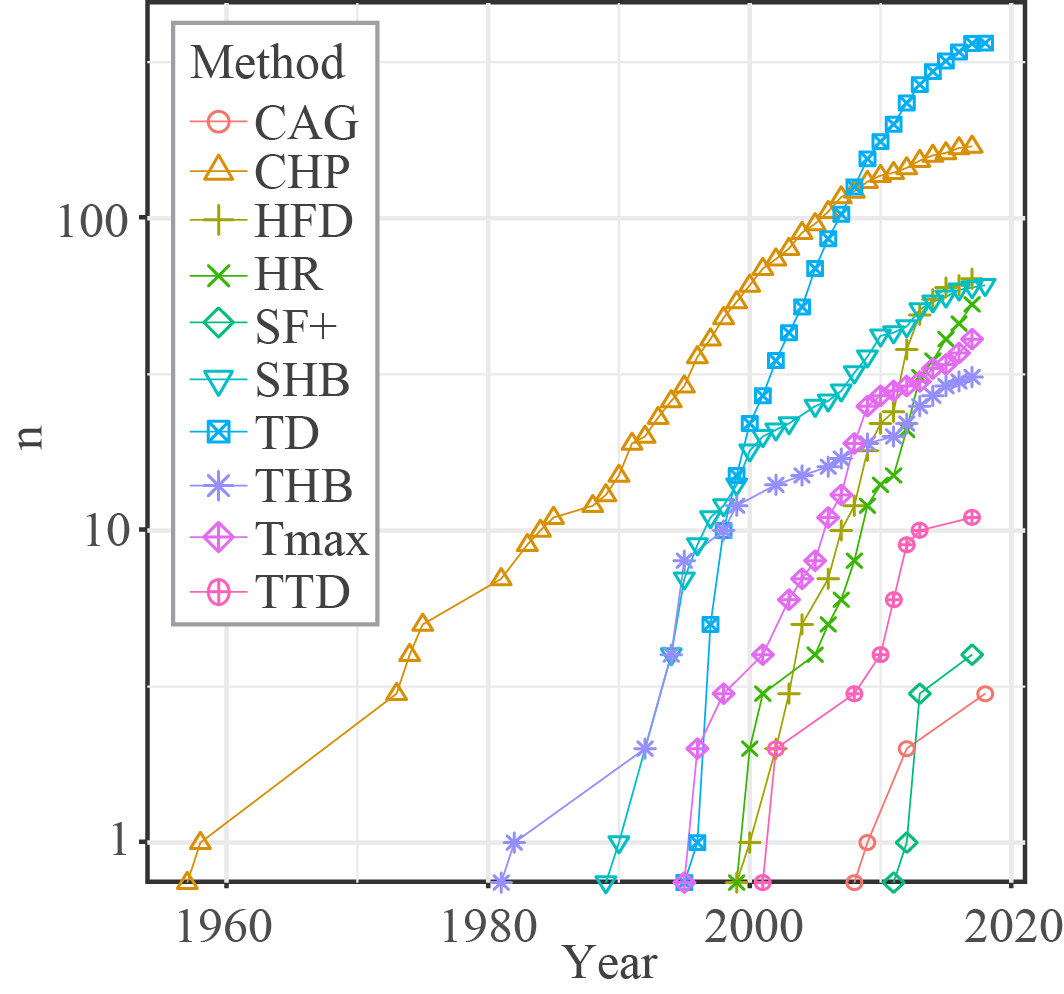
\includegraphics[width=0.9\linewidth]{figure/appendixA1/fig1} 

}

\caption[Multivariate Environmental Similarity Surface (MESS) analyses ninyerola vs worlclim methods]{ Multivariate Environmental Similarity Surface (MESS) analysis between Worldclim data base and Spanish climatic data base following  Ninyerola and others 2000 and climatic data from iberian climatic atlas for 1950-2000 period. Negative values mean dissimilarities between the two data bases. BIO3= Isothermality, BIO4= Temperature Seasonality, BIO8= Mean Temperature of Wettest Quarter, BIO9= Mean Temperature of Driest Quarter, BIO12= Annual Precipitation and BIO15= Precipitation Seasonality.}\label{fig:apa11}
\end{figure}
\setlength{\abovecaptionskip}{0pt}
\newpage
\end{landscape}
\begin{center}\includegraphics[width=0.8\linewidth]{figure/appendixA1/fig2primeraparte} \end{center}

\setlength{\textfloatsep}{-10pt plus 1.0pt minus 2.0pt}

\setlength{\abovecaptionskip}{15pt}
\begin{figure}[hbt!]

{\centering \includegraphics[width=0.8\linewidth]{figure/appendixA1/fig2segundaparte} 

}

\caption[ AUC and Boyce index per species]{ Above: Area Under ROC Curve (AUC) by specie and models. Vertical lines represent AUC standard deviation interval of each model while horizontal lines show AUC mean values. Below: Boyce index values by specie and models. Vertical lines represent standard deviation for Boyce values while horizontal lines show Boyce mean values. Notice that the species order is different for each plot.}\label{fig:apa122}
\end{figure}
\setlength{\abovecaptionskip}{0pt}

\newpage
\begin{landscape}
\begin{figure}[hbt!]

{\centering 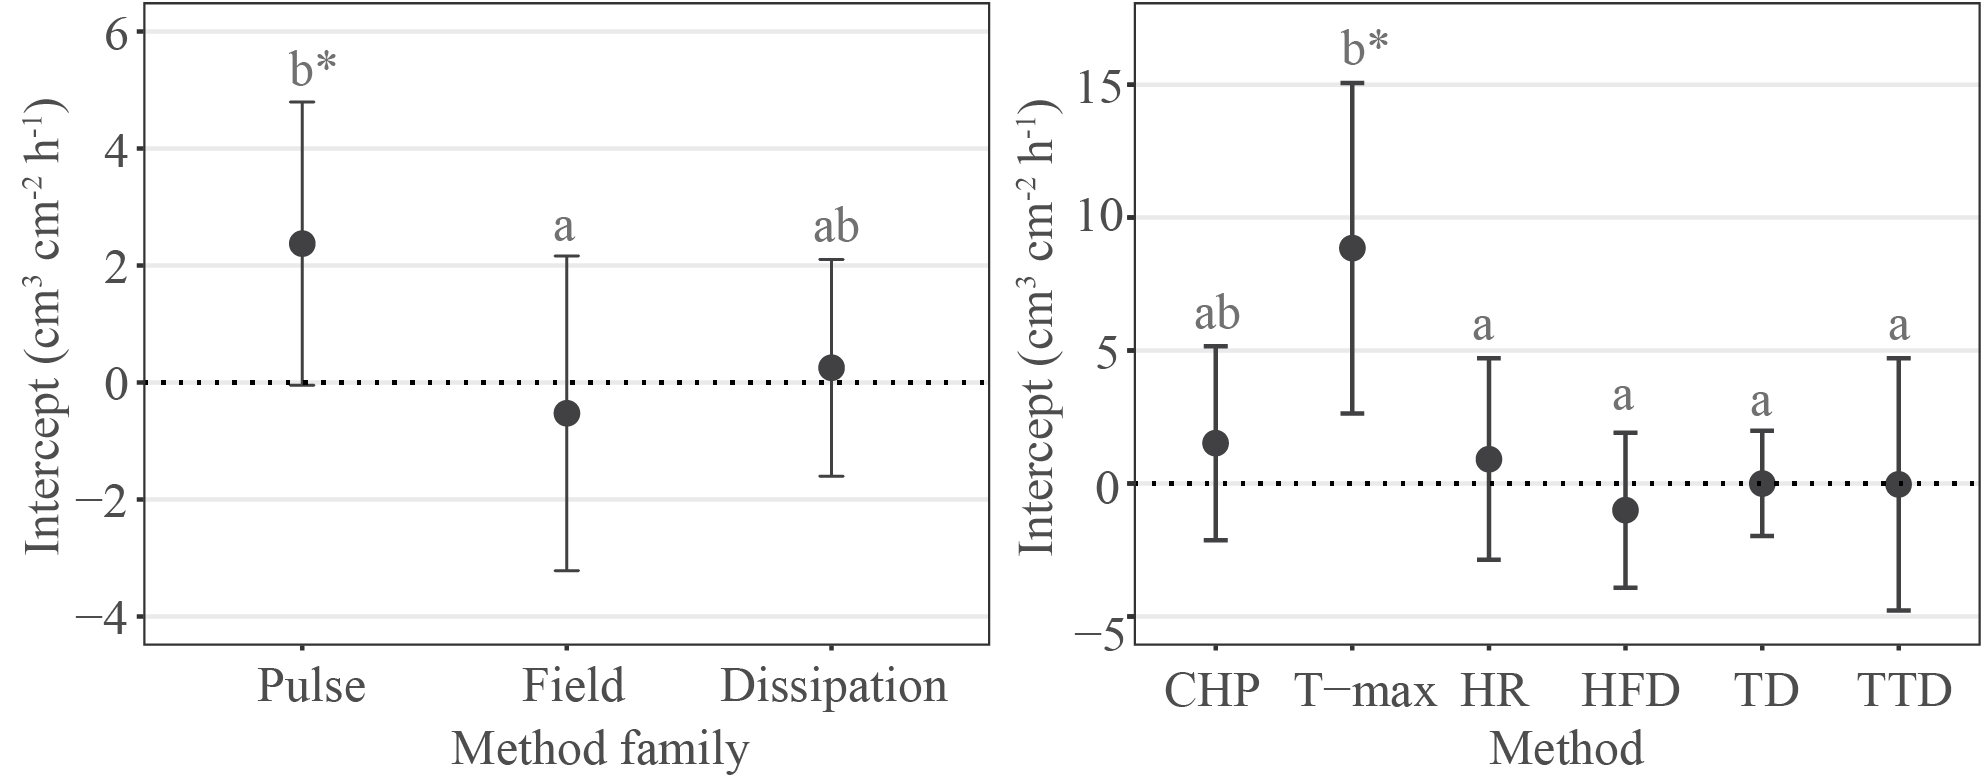
\includegraphics[width=0.8\linewidth]{figure/appendixA1/fig3} 

}

\caption[Multivariate Environmental Similarity Surface (MESS) analyses of the extreme drought year]{Multivariate Environmental Similarity Surface (MESS) analysis for the Region of Murcia. Bio3 to Bio15 shows the similarity between the new environment (extreme episode 2013-2014) and the environments use to calibrate the model (historic period 1950-2000) for each different variables  implemented  in  the  models. BIO3= Isothermality, BIO4= Temperature Seasonality, BIO8= Mean Temperature of Wettest Quarter, BIO9= Mean Temperature of Driest Quarter, BIO12= Annual Precipitation and BIO15= Precipitation Seasonality. Negative values are  indicative  of  environmental dissimilarities  between variables.  Note that bio15 (precipitation seasonality) is  the main contributor to final MESS. Black square represents the study site location.}\label{fig:apa13}
\end{figure}
\begin{figure}[hbt!]

{\centering \includegraphics[width=0.8\linewidth]{figure/appendixA1/fig4} 

}

\caption[Historic Climatic Suitability (HCS) averaged values of the sample plots by species for each implemented model]{Historic Climatic Suitability (HCS) averaged values of the sample plots by species for each implemented model.}\label{fig:apa14}
\end{figure}
\newpage
\end{landscape}\begin{figure}[hbt!]
{\centering \includegraphics[width=1.2\linewidth]{figure/appendixA1/fig5} 

}

\caption[Pearson correlation values among different implemented models for HCS]{Pearson correlation values among different implemented models for Historic Climatic Suitability (HCS). Significant values are highlighted in bold. Correlation plots are also shown}\label{fig:apa15}
\end{figure}\newpage
\begin{figure}[hbt!]

{\centering \includegraphics[width=1.2\linewidth]{figure/appendixA1/fig6} 

}

\caption[Pearson correlation values among different implemented models for Episodic Climatic Suitability (ECS)]{Pearson correlation values among different implemented models for Episodic Climatic Suitability (ECS). Significant values are highlighted in bold. Correlation plots are also shown.}\label{fig:apa16}
\end{figure}
\newpage

\setlength{\abovecaptionskip}{0pt}
\begin{center}\includegraphics[width=1\linewidth]{figure/appendixA2/annex2fig1primeraparte} \end{center}

\setlength{\textfloatsep}{-10pt plus 1.0pt minus 2.0pt}
\begin{figure}[hbt!]

{\centering \includegraphics[width=1\linewidth]{figure/appendixA2/annex2fig1segundaparte} 

}

\caption[ Filtered occurences of analized species]{ Filtered occurences of every analized species.}\label{fig:apa212}
\end{figure}
\newpage
\begin{landscape}
\begin{center}\includegraphics[width=0.9\linewidth]{figure/appendixA2/figure2/parte1} \end{center}

\begin{center}\includegraphics[width=0.9\linewidth]{figure/appendixA2/figure2/parte2} \end{center}

\begin{center}\includegraphics[width=0.9\linewidth]{figure/appendixA2/figure2/parte3} \end{center}
\setlength{\textfloatsep}{-10pt plus 1.0pt minus 2.0pt}

\setlength{\abovecaptionskip}{15pt}
\begin{figure}[hbt!]

{\centering \includegraphics[width=0.9\linewidth]{figure/appendixA2/figure2/parte4} 

}

\caption[Suitability maps obtained from Mahalanobis distance]{Suitability maps obtained from Mahalanobis distance. Note that Mediterranean basin maps were used to project the models under 1950-2000 average conditions, while Region of Murcia maps were used to project the models under extreme hydrological year 2013-2014.}\label{fig:apa224}
\end{figure}
\setlength{\abovecaptionskip}{0pt}

\newpage
\end{landscape}
\newpage
\begin{landscape}
\begin{center}\includegraphics[width=0.9\linewidth]{figure/appendixA2/figure3/parte1} \end{center}

\begin{center}\includegraphics[width=0.9\linewidth]{figure/appendixA2/figure3/parte2} \end{center}

\begin{center}\includegraphics[width=0.9\linewidth]{figure/appendixA2/figure3/parte3} \end{center}
\setlength{\textfloatsep}{-10pt plus 1.0pt minus 2.0pt}

\setlength{\abovecaptionskip}{15pt}
\begin{figure}[hbt!]

{\centering \includegraphics[width=0.9\linewidth]{figure/appendixA2/figure3/parte4} 

}

\caption[Suitability maps obtained from Generalize Additive Models (GAM)]{Suitability maps obtained from Generalize Additive Models (GAM). Note that Mediterranean basin maps were used to project the models under 1950-2000 average conditions, while Region of Murcia maps were used to project the models under extreme hydrological year 2013-2014.}\label{fig:apa234}
\end{figure}
\setlength{\abovecaptionskip}{0pt}

\newpage
\end{landscape}
\newpage
\begin{landscape}
\begin{center}\includegraphics[width=0.9\linewidth]{figure/appendixA2/figure4/parte1} \end{center}

\begin{center}\includegraphics[width=0.9\linewidth]{figure/appendixA2/figure4/parte2} \end{center}

\begin{center}\includegraphics[width=0.9\linewidth]{figure/appendixA2/figure4/parte3} \end{center}
\setlength{\textfloatsep}{-10pt plus 1.0pt minus 2.0pt}

\setlength{\abovecaptionskip}{15pt}
\begin{figure}[hbt!]

{\centering \includegraphics[width=0.9\linewidth]{figure/appendixA2/figure4/parte4} 

}

\caption[Suitability maps obtained from Boosted Regression Trees (BRT)]{Suitability maps obtained from Boosted Regression Trees (BRT). Note that Mediterranean basin maps were used to project the models under 1950-2000 average conditions, while Region of Murcia maps were used to project the models under extreme hydrological year 2013-2014.}\label{fig:apa244}
\end{figure}
\setlength{\abovecaptionskip}{0pt}

\newpage
\end{landscape}
\newpage
\begin{landscape}
\begin{center}\includegraphics[width=0.9\linewidth]{figure/appendixA2/figure5/parte1} \end{center}

\begin{center}\includegraphics[width=0.9\linewidth]{figure/appendixA2/figure5/parte2} \end{center}

\begin{center}\includegraphics[width=0.9\linewidth]{figure/appendixA2/figure5/parte3} \end{center}
\setlength{\textfloatsep}{-10pt plus 1.0pt minus 2.0pt}


\setlength{\abovecaptionskip}{15pt}
\begin{figure}[hbt!]

{\centering \includegraphics[width=0.9\linewidth]{figure/appendixA2/figure5/parte4} 

}

\caption[Suitability maps obtained from MaxEnt]{Suitability maps obtained from MaxEnt. Note that Mediterranean basin maps were used to project the models under 1950-2000 average conditions, while Region of Murcia maps were used to project the models under extreme hydrological year 2013-2014.}\label{fig:apa254}
\end{figure}
\setlength{\abovecaptionskip}{0pt}

\newpage
\end{landscape}
\setlength{\abovecaptionskip}{15pt}
\begin{table}[H]

\caption[Pearson correlation values comparing visual drought estimates and defoliation]{\label{tab:unnamed-chunk-11}Pearson correlation values comparing visual drought estimate and defoliation directly measure by centimeters, for each measured species. N is the number of measured individual for all study site.}
\centering
\fontsize{8}{10}\selectfont
\begin{tabular}[t]{lrr}
\toprule
Species & N & Pearson corr\\
\midrule
Anthyllis cytisoides & 60 & 0.919\\
Artemisia barrelieri & 90 & 0.938\\
Artemisia campestris & 10 & 0.966\\
Asparagus horridus & 10 & 0.935\\
Cistus albidus & 10 & 0.701\\
Cistus clusii & 86 & 0.978\\
Daphne gnidium & 20 & 0.720\\
Dorycnium pentaphyllum & 50 & 0.935\\
Fumana ericoides & 90 & 0.984\\
Helianthemum syriacum & 30 & 0.935\\
Juniperus oxycedrus & 44 & 0.899\\
Juniperus phoenicea & 10 & 0.901\\
Lithodora fruticosa & 10 & 0.882\\
Ononis fruticosa & 40 & 0.851\\
Pistacia lentiscus & 50 & 0.889\\
Quercus coccifera & 70 & 0.961\\
Rhamnus lycioides & 25 & 0.890\\
Rosmarinus officinalis & 100 & 0.860\\
Salsola genistoides & 15 & 0.821\\
Sideritis leucantha & 13 & 0.880\\
Stippa tenacissima & 100 & 0.952\\
Teucrium  capitatum gracillimum & 44 & 0.873\\
Thymus hyemalis & 100 & 0.946\\
\bottomrule
\end{tabular}
\end{table}
\setlength{\abovecaptionskip}{0pt}

\setlength{\abovecaptionskip}{15pt}
\begin{table}[H]

\caption[Median and range values for Historical Climatic Suitability and Episode Climatic Suitability]{\label{tab:unnamed-chunk-12}Median and range values for Historical Climatic Suitability (HCS) and Episode Climatic Suitability (ECS) of different SDM applied for the co-occurring species in the studied community.}
\centering
\fontsize{8}{10}\selectfont
\begin{tabular}[t]{lllll}
\toprule
  & mahal & GAM & BRT & MaxEnt\\
\midrule
HCS range & 0.902 - 0.031 & 0.965 - 0.613 & 0.992 - 0.332 & 0.751 - 0.121\\
HCS median & 0.5423 & 0.845 & 0.8527 & 0.3632\\
ECS range & 8.267x10-7 - 0 & 0.303 - 2.22x10-16 & 0.104 - 1.26x10-3 & 0.084 - 1.51x10-5\\
ECS median & 4.83x10-16 & 0.0032 & 0.0053 & 0.0034\\
\bottomrule
\end{tabular}
\end{table}
\setlength{\abovecaptionskip}{0pt}

\chapter{Appendix Chapter 3}\label{appendix-chapter-3}

\newpage

\setlength{\abovecaptionskip}{10pt}
\begin{figure}[hbt!]

{\centering \includegraphics[width=1\linewidth]{figure/appendixB/figure1} 

}

\caption[ Climatic anomaly of the extreme climatic year 2013-2014 in the Spanish SE]{Climatic anomaly of the extreme climatic year 2013-2014 in the Spanish SE. Temperature anomaly is measured as degrees change respect to the average for the period 1970-2000, while precipitation anomaly is estimated as relative change (\%) respect to the average period 1970-2000.}\label{fig:apc1}
\end{figure}\newpage
\begin{figure}[hbt!]

{\centering \includegraphics[width=1.2\linewidth]{figure/appendixB/figure2} 

}

\caption[Correlation circle obtained from PCA calibrated with $Pinus$ $halepnsis$ occurrences]{Correlation circle obtained from PCA from the twelve selected climatic variables. Where BIO1= Annual Mean Temperature, BIO4= Temperature Seasonality (standard deviation×100), BIO5= Max Temperature of Warmest Month, BIO6= Min Temperature of Coldest Month, BIO10= Mean Temperature of Warmest Quarter, BIO11= Mean Temperature of Coldest Quarter, BIO12= Annual Precipitation, BIO13= Precipitation of Wettest Month, BIO14= Precipitation of Driest Month, BIO15= Precipitation Seasonality (Coefficient of Variation), BIO16= Precipitation of Wettest Quarter, BIO17= Precipitation of Driest Quarter. The PCA was calibrated using climatic data from the total filtered 9,959 occurrences of $Pinus$ $halepensis$ occurrences from the Spanish National Forest Inventory (IFN).  First and second axes contained 60\% of explained variability. The variables' color represents the percentage of each variable' contribution to the PCA.}\label{fig:apc2}
\end{figure}\newpage
\begin{figure}[hbt!]

{\centering \includegraphics[width=1\linewidth]{figure/appendixB/figure3} 

}

\caption[Populations located in the $Pinus$ niche space not shared by the average-based and the inter-annual variability-based niches]{Populations located in the niche space that is not shared by the average-based and the inter-annual variability-based niches. Orange region represents the area of the variability-based niche that is not included within the average-based niche area.}\label{fig:apc3}
\end{figure}\newpage
\begin{figure}[hbt!]

{\centering \includegraphics[width=1\linewidth]{figure/appendixB/figure4pp200} 

}

\caption[Model explained $R^2$ depending on population subset]{Model explained $R^2$ depending on population subset, where response variable was plot mortality percentage and explanatory variables was plot climatic suitability. X axis ranged from 0 percentage of population located in the non-shared niche space by inter-annual and average-based niches to 100. Blue color represent $R^2$ values obtained with climatic suitability derived from the average-based niche while yellow color represent $R^2$ values obtained with climatic suitability derived from the inter-annual variability-based niche.}\label{fig:apc4}
\end{figure}\newpage
\begin{figure}[hbt!]

{\centering \includegraphics[width=0.9\linewidth]{figure/appendixB/figure5} 

}

\caption[Correlation circle obtained from PCA calibrated with occurrences of multiples mediterranean species]{Correlation circle obtained from PCA from the twelve selected climatic variables. Where BIO1= Annual Mean Temperature, BIO4= Temperature Seasonality (standard deviation×100), BIO5 = Max Temperature of Warmest Month, BIO6= Min Temperature of Coldest Month, BIO10 = Mean Temperature of Warmest Quarter, BIO11= Mean Temperature of Coldest Quarter, BIO12= Annual Precipitation, BIO13= Precipitation of Wettest Month, BIO14 = Precipitation of Driest Month, BIO15= Precipitation Seasonality (Coefficient of Variation), BIO16= Precipitation of Wettest Quarter, BIO17 = Precipitation of Driest Quarter. The PCA was calibrated using climatic data from the total filtered 116,835 occurrences from the Spanish National Forest Inventory (IFN) and gbif.org for all the 42 selected species.  First and second axes contained 60.8\% of explained variability. The variables' color represents the percentage of each variable' contribution to the PCA.}\label{fig:apc5}
\end{figure}\newpage
\begingroup\fontsize{7}{9}\selectfont
\begin{longtable}[t]{lrrrl}
\caption[Species used for analyses of changes in niche space depending on species climatic range]{\label{tab:unnamed-chunk-13}Species used for analyses of changes in niche space depending on species climatic range. Table shows area of average based-niche (niche area av), inter-annual based-niche (niche area in), niche rate (area of average based-niche/area of inter-annual variability based-niche) and species’ distribution range, where endemic SE means species endemic from the Spanish south east and mediterraneean occ means species mostly distributed in the west of the Mediterranean basin.}\\
\toprule
Species & Niche area av & Niche area in & Niche rate & Distr range\\
\midrule
\endfirsthead
\caption[]{\label{tab:unnamed-chunk-13}Species used for analyses of changes in niche space depending on species climatic range. Table shows area of average based-niche (niche area av), inter-annual based-niche (niche area in), niche rate (area of average based-niche/area of inter-annual variability based-niche) and species’ distribution range, where endemic SE means species endemic from the Spanish south east and mediterraneean occ means species mostly distributed in the west of the Mediterranean basin. \textit{(continued)}}\\
\toprule
Species & Niche area av & Niche area in & Niche rate & Distr range\\
\midrule
\endhead
\
\endfoot
\bottomrule
\endlastfoot
Anthyllis terniflora & 8.185 & 21.856 & 2.670 & endemic SE\\
Artemisia barrelieri & 12.619 & 34.393 & 2.725 & endemic SE\\
Asparagus horridus & 37.065 & 59.544 & 1.606 & mediterranean\\
Chamaerops humilis & 19.124 & 39.579 & 2.070 & iberoafrican\\
Cistus clusii & 15.010 & 35.679 & 2.377 & mediterranean occ\\
Cistus monspeliensis & 35.642 & 64.681 & 1.815 & mediterranean\\
Coronilla juncea & 19.049 & 39.719 & 2.085 & mediterranean occ\\
Dorycnium pentaphyllum & 33.890 & 61.624 & 1.818 & mediterranean occ\\
Frankenia corymbosa & 8.917 & 26.437 & 2.965 & iberoafrican\\
Fumana ericoides & 35.136 & 65.437 & 1.862 & mediterranean occ\\
Fumana laevipes & 19.356 & 39.366 & 2.034 & mediterranean occ\\
Fumana thymifolia & 35.459 & 62.157 & 1.753 & mediterranean\\
Genista valentina & 8.635 & 30.559 & 3.539 & endemic SE\\
Globularia alypum & 22.391 & 46.018 & 2.055 & mediterranean\\
Helianthemum syriacum & 18.758 & 39.410 & 2.101 & mediterranean\\
Helianthemum violaceum & 18.513 & 40.585 & 2.192 & iberoafrican\\
Helianthemum viscarium & 6.997 & 21.046 & 3.008 & iberoafrican\\
Helichrysum stoechas & 31.154 & 56.958 & 1.828 & mediterranean\\
Hyparrhenia hirta & 31.256 & 58.032 & 1.857 & iberoafrican\\
Launaea arborescens & 22.925 & 46.767 & 2.040 & iberoafrican\\
Launaea lanifera & 9.986 & 25.835 & 2.587 & iberoafrican\\
Lavandula dentata & 26.418 & 47.171 & 1.786 & iberoafrican\\
Lycium intricatum & 13.456 & 33.463 & 2.487 & iberoafrican\\
Lygeum spartum & 16.895 & 35.325 & 2.091 & iberoafrican\\
Paronychia suffruticosa & 23.259 & 50.011 & 2.150 & endemic SE\\
Periploca angustifolia & 6.763 & 25.751 & 3.808 & iberoafrican\\
Phagnalon rupestre & 43.312 & 70.418 & 1.626 & mediterranean\\
Phagnalon saxatile & 37.291 & 62.075 & 1.665 & mediterranean\\
Pinus halepensis & 20.781 & 41.029 & 1.974 & mediterranean occ\\
Rhamnus lycioides & 34.148 & 60.770 & 1.780 & mediterranean\\
Rosmarinus officinalis & 35.674 & 62.756 & 1.759 & mediterranean\\
Salsola genistoides & 6.980 & 20.683 & 2.963 & endemic SE\\
Salsola oppositifolia & 10.617 & 24.630 & 2.320 & iberoafrican\\
Salsola papillosa & 4.144 & 14.237 & 3.435 & endemic SE\\
Satureja obovata & 17.471 & 40.550 & 2.321 & mediterranean occ\\
Sideritis ibanyezii & 3.161 & 12.455 & 3.940 & endemic SE\\
Stipa tenacissima & 18.355 & 37.528 & 2.045 & iberoafrican\\
Teucrium capitatum & 14.707 & 31.387 & 2.134 & mediterranean occ\\
Teucrium freynii & 5.638 & 17.164 & 3.044 & endemic SE\\
Teucrium lanigerum & 3.424 & 13.174 & 3.847 & endemic SE\\
Thymelaea hirsuta & 22.451 & 44.471 & 1.981 & mediterranean\\
Thymus hyemalis & 5.540 & 18.523 & 3.344 & endemic SE\\*
\end{longtable}
\endgroup{}
\begin{table}[H]

\caption[GLM binomial model results relating $Pinus$ decay with species climatic niche suitability]{\label{tab:unnamed-chunk-14}GLM binomial model results relating species decay (as binary or continuous response) with species niche suitability obtained from average-based and from inter-annual variability-based models. Models $R^2$ and AIC are given in the main text (Figure 3.3).}
\centering
\fontsize{8}{10}\selectfont
\begin{tabular}[t]{lllrrl}
\toprule
Dataset & Response & Explanatory & Estimate & SE & Pvalue\\
\midrule
interannual & binary & intercept & -0.58 & 0.05 & <0.001\\
 &  & suitability & -4.40 & 0.26 & <0.001\\
interannual & continuous & intercept & -0.53 & 0.19 & 0.006\\
 &  & suitability & -5.70 & 1.40 & <0.001\\
average & binary & intercept & -1.02 & 0.04 & <0.001\\
 &  & suitability & -3.80 & 0.28 & <0.001\\
average & continuous & intercept & -0.84 & 0.16 & <0.001\\
 &  & suitability & -7.02 & 2.08 & <0.001\\
\bottomrule
\end{tabular}
\end{table}
\begin{table}[H]

\caption[Model results relating models explanatory capacity in relation to the percentage of populations located in the non-shared niche space]{\label{tab:unnamed-chunk-15}Model results relating models explanatory capacity ($R^2$) in relation to the percentage of populations located in the non-shared area between the two niche estimations (average-based and inter-annual variability-based niche). $R^2$ were obtained by models that relate decay records as continuous response with different subsets of the records, in order to simulate the different percentages of population located in the non-shared area. Explanatory variables of the model are: corona percentage (percentage of population located in the non-shared niches area), niche model (averaged-based or inter-annual variability-based and n (number of records of the model, which varies from 118 to 264).}
\centering
\fontsize{8}{10}\selectfont
\begin{tabular}[t]{lllll}
\toprule
Explanatory & Estimate & SE & Pvalue & $R^2$= 0.954\\
\midrule
Intercept & 0.387 & 0.000472 & <0.001 & \\
corona\,percentage & -0.379 & 0.000457 & <0.001 & \\
dataset\, interannual & 0.0157 & 0.000331 & <0.001 & \\
n & 2.18x10-5 & 1.5x10-6 & <0.001 & \\
Corona\, percentage : dataset\, interannual & 0.0872 & 0.000632 & <0.001 & \\
\bottomrule
\end{tabular}
\end{table}
\par
\begin{table}[H]

\caption[Model results relating relating ratio of niche area and niche average size]{\label{tab:unnamed-chunk-16}Model results with ratio of niche area (inter-annual variability-based niche area/average-based area) as response variable and log(average-based niche area) and distribution range as explanatory variables. }
\centering
\fontsize{8}{10}\selectfont
\begin{tabular}[t]{lrrll}
\toprule
Explanatory & Estimate & SE & Pvalue & $R^2 = 0.895$\\
\midrule
Intercept (SE endemic) & 4.79 & 0.16 & <0.001 & \\
Log(niche area average) & -0.85 & 0.08 & <0.001 & \\
Distrib\,ib\,af & -0.12 & 0.11 & 0.279 & \\
Distrib\,med & -0.06 & 0.15 & 0.701 & \\
Distrib\,med\,occ & -0.14 & 0.13 & 0.299 & \\
\bottomrule
\end{tabular}
\end{table}
\chapter{Appendix Chapter 4}\label{appendix-chapter-4}

\newpage

\setlength{\abovecaptionskip}{10pt}
\begin{figure}[hbt!]

{\centering \includegraphics[width=1\linewidth]{figure/appendixD/figure1} 

}

\caption[Ombrothermic diagrams for the study site]{Ombrothermic diagrams for A) Cuatro Calas, B) Moreras Mountain and C) Calblanque Natural Park, respectively. Red lines correspond to temperatures, and blue lines correspond to precipitation. Solid lines correspond to the reference climatic period (1979-2012, Chelsa v.1.2, Karger et al. 2017) and dotted lines correspond to extreme climatic year (2013-2014) (data from Spanish Weather Agency, AEMET). Vertical blue and red lines over the reference period lines show Standard Error estimated for each month in the period 1979-2012.}\label{fig:unnamed-chunk-17}
\end{figure}\newpage
\begin{figure}[hbt!]

{\centering \includegraphics[width=0.8\linewidth]{figure/appendixD/figure2} 

}

\caption[Soil particle composition of the study sites]{Soil particle composition of the three different study sites’ bedrocks (i.e., Moreras’ Mountain, Calblanque Natural Parck, and Cuatro Calas, respectively to this graphic order. Yellow colour represents the proportion of sands, orange the proportion of clays and 30 dark orange the proportion of silts.}\label{fig:unnamed-chunk-18}
\end{figure}\newpage
\begin{figure}[hbt!]

{\centering \includegraphics[width=1\linewidth]{figure/appendixD/figure3} 

}

\caption[Correlation circle obtained from PCA from the twelve selected climatic variables.]{Correlation circle obtained from PCA from the twelve selected climatic variables. Where BIO1 = Annual Mean Temperature, BIO4 = Temperature Seasonality (standard deviation×100), BIO5 = Max Temperature of Warmest Month, BIO6 = Min Temperature of Coldest Month, BIO10= Mean Temperature of Warmest Quarter, BIO11 = Mean Temperature of Coldest Quarter, BIO12 = Annual Precipitation, BIO13 = Precipitation of Wettest Month, BIO14 = Precipitation of Driest Month, BIO15 = Precipitation Seasonality (Coefficient of Variation), BIO16 = Precipitation of Wettest Quarter, BIO17 = Precipitation of Driest Quarter. The PCA was calibrated using climatic data from the total filtered 106,876 occurrences from gbif.org for all the 38 sampled species. The first and second axes contained 60.8\% of explained variability. The variables' colour represents the percentage of each variable' contribution to the PCA.}\label{fig:unnamed-chunk-19}
\end{figure}\newpage
\begin{figure}[hbt!]

{\centering \includegraphics[width=1\linewidth]{figure/appendixD/figure4} 

}

\caption[Correlation circle obtained from PCA calibrated with the five climatic variables used in SDMs]{Correlation circle obtained from PCA calibrated with the five climatic variables included in SDMs (MaxEnt) using climatic data from the total filtered 106,876 occurrences from gbif.org for all the 38 sampled species. In order to discard difference between environmental spaces calibrated with the first 12 variables (Figure S3) instead of this 6 variables. We calculated the pearson correlation between the contribution of these 6 variables in both calibrated pca. We obtained a correlation of -0.9425 for axis 1, and 0.9115 for axis 2. BIO1 = Annual Mean Temperature, BIO4 = Temperature Seasonality (standard deviation×100), BIO10 = Mean Temperature of Warmest Quarter, BIO12 = Annual Precipitation, BIO15 = Precipitation Seasonality (Coefficient of Variation), BIO17 = Precipitation of Driest Quarter. The PCA was calibrated using climatic data from the total filtered 106,876 occurrences from gbif.org for all the 38 sampled species. The first and second axes contained 63.6\% of explained variability. The variables' colour represents the percentage of each variable' contribution to the PCA. }\label{fig:unnamed-chunk-20}
\end{figure}\newpage
\begin{figure}[hbt!]

{\centering \includegraphics[width=1.1\linewidth]{figure/appendixD/figure5} 

}

\caption[Remaining Green Canopy (RGC) and mortality percentage models]{Remaining Green Canopy (RGC) in relation to population distances during the reference period 1979-2012 to their respective species niche centroid (A) and to the closest point of the niche limit (B); Mortality percentage in relation to population distances during the reference period 1979-2012 to their respective species niche centroid (C) and to the closest point of the niche limit (D). In all four cases, only the subset of populations located within the niche were considered. Yellow dots show distances of populations located in Moreras’ Mountain (limestone bedrock), magenta dots show distances of populations located in Calblanque Natural Parck (metamorphic bedrock) and blue dots show distances of populations located in Cuatro Calas (sandstone bedrock). Yellow, magenta and blue lines represent the regression lines of the model for each bedrock type. Each panel also shows $R^2$ model values and ANOVA P-values (Pv) for testing significance of niche distances.}\label{fig:unnamed-chunk-21}
\end{figure}\newpage
\begin{figure}[hbt!]

{\centering \includegraphics[width=1\linewidth]{figure/appendixD/figure6} 

}

\caption[Multivariate Environmental Similarity Surface (MESS) analysis for the South East of the Iberian Peninsula.]{Multivariate Environmental Similarity Surface (MESS) analysis for the South East of the Iberian Peninsula. We calculated the median similarity between the new environment (extreme episode 2013-2014) and the environment used to fit each species model (average reference period 1979-2012 CHELSA database) for each variable implemented in our models. Negative values are indicative of high environmental dissimilarities between variables.}\label{fig:unnamed-chunk-22}
\end{figure}
\newpage
\begin{table}[H]

\caption[Carbon and nitrogen content of each studied bedrock, following (Anne 1945, Duchaufour 1970) method.]{\label{tab:unnamed-chunk-23}Carbon and nitrogen content of each studied bedrock, following (Anne 1945, Duchaufour 1970) method.}
\centering
\fontsize{8}{10}\selectfont
\begin{tabular}[t]{lllrrr}
\toprule
Bedrock & Locality & Replicate & Organic C (g/100g) & Total N (g/100g) & C:N ratio\\
\midrule
 &  & C1 & 1.42 & 0.19 & 7.47\\
Metamorphic & Calblanque & C2 & 1.22 & 0.17 & 7.18\\
 &  & C3 & 3.91 & 0.31 & 12.61\\
 &  & H1 & 0.71 & 0.06 & 11.83\\
Sandstone & Cuatro Calas & H2 & 0.94 & 0.09 & 10.44\\
 &  & H3 & 1.09 & 0.09 & 12.11\\
 &  & M1 & 3.17 & 0.35 & 9.06\\
Limestone & Moreras & M2 & 1.83 & 0.22 & 8.32\\
 &  & M3 & 2.52 & 0.23 & 10.96\\
\bottomrule
\end{tabular}
\end{table}
\newpage
\begin{table}[H]

\caption[Summary table of analysed species]{\label{tab:unnamed-chunk-24}Summary table of analysed species found in the different study sites. The table shows the species codes used in climatic diagrams and the species families, as well as the study area in which they were found. In the latter column, S represents Cuatro Calas area (sandstone bedrock), M Calblanque area (metamorphic bedrock) and L Moreras Mountain area (limestone bedrock).}
\centering
\fontsize{8}{10}\selectfont
\begin{tabular}[t]{llll}
\toprule
SPECIES NAME & SPECIES CODE & FAMILY & LOCALITY\\
\midrule
Anthyllis terniflora & ATER & Leguminosae & S\\
Artemisia barrelieri & ABAR & Asteraceae & S, M\\
Asparagus horridus & AHOR & Asparagaceae & S, L, M\\
Chamaerops humilis & CHUM & Arecaceae & M\\
Cistus Clusii & CCLU & Cistaceae & S, M\\
Cistus monspeliensis & CMON & Cistaceae & M\\
Coronilla juncea & CJUN & Leguminosae & M\\
Dorycnium pentaphyllum & DPEN & Leguminosae & M\\
Frankenia corymbosa & FCOR & Frankeniaceae & S, M\\
Fumana ericoides & FERI & Cistaceae & S, L, M\\
Fumana laevipes & FLAE & Cistaceae & L, M\\
Fumana thymifolia & FTHY & Cistaceae & L\\
Genista valentina & GVAL & Leguminosae & L\\
Globularia alypum & GALY & Plantaginaceae & L\\
Helianthemum syriacum & HSYR & Cistaceae & M\\
Helianthemum violaceum & HVIO & Cistaceae & S, L\\
Helianthemum viscarium & HVIS & Cistaceae & S\\
Hyparrhenia hirta & HHIR & Poaceae & L\\
Launaea arborescens & LARB & Asteraceae & S, L, M\\
Launaea lanifera & LLAN & Asteraceae & S, L\\
Lavandula dentata & LDEN & Lamiaceae & S\\
Lycium intricatum & LINT & Solanaceae & S, M\\
Lygeum spartum & LSPA & Poaceae & M\\
Paronychia suffruticosa & PSUF & Caryophillaceae & M\\
Periploca angustifolia & PANG & Apocynaceae & S, L\\
Rosmarinus officinalis & ROFF & Lamiaceae & S, L, M\\
Salsola genistoides & SGEN & Amaranthaceae & S, L\\
Salsola oppositifolia & SOPP & Amaranthaceae & S\\
Salsola papillosa & SPAP & Amaranthaceae & M\\
Satureja obovata & SOBO & Lamiaceae & L\\
Sideritis ibanyezii & SIBA & Lamiaceae & S, M\\
Stipa tenacissima & STEN & Poaceae & S, L, M\\
Teucrium capitatum & TCAP & Lamiaceae & S, M\\
Teucrium freynii & TFRE & Lamiaceae & L\\
Teucrium lanigerum & TLAN & Lamiaceae & S, L\\
Thymelaea hirsuta & THIR & Thymelaeaceae & S, L, M\\
Thymus hyemalis & THYE & Lamiaceae & S, L, M\\
\bottomrule
\end{tabular}
\end{table}
\newpage
\begin{table}[H]

\caption[Final generalized mix models applied for Remaining Green Canopy (RGC) and mortality respectively.]{\label{tab:unnamed-chunk-25}Final generalized mix models applied for Remaining Green Canopy (RGC) and mortality respectively.}
\centering
\fontsize{7}{9}\selectfont
\begin{tabular}[t]{lll}
\toprule
Response variable & Explanatory variables & Random effects\\
\midrule
RGC & $centroid\, distance\, av\, +\, lithology\, +\, centroid\, distance\, av :\, lithology$ & $species + plot$\\
RGC & $limit\, distance\, av\, :\, in\, out\, av\, +\, lithology$ & $species + plot$\\
mortality & $centroid\, distance\, av\, +\, lithology$ & $species + plot$\\
mortality & $limit\, distance\, av\, :\,in\, out\, av\,+\, lithology$ & $species + plot$\\
RGC & $centroid\, distance\, av\, +\, lithology\, +\, centroid\, distance\, av\, :\, lithology$ & $species + plot$\\
RGC & $limit distance\, av\, :\, in\, out\, av\, +\, lithology$ & $species + plot$\\
mortality & $centroid\, distance\, av\, +\, lithology$ & $species + plot$\\
mortality & $limit\, distance\, av\,:\,in\, out\, av\, +\, lithology$ & $species + plot$\\
RGC & $climatic\, suitability\, av\, +\, lithology\, +\, climatic\, suitability\, av\,:\, lithology$ & $species + plot$\\
RGC & $climatic\, suitability\, ex\, +\, lithology$ & $species + plot$\\
\bottomrule
\end{tabular}
\end{table}
\begin{table}[H]

\caption[Model accuracy of each sampled species distribution model estimated with MaxEnt.]{\label{tab:unnamed-chunk-26}Model accuracy of each sampled species distribution model estimated with MaxEnt. AUC column shows average of 5 alternative models (5-fold cross-validation) and Sd-AUC column shows the standard deviation of AUC values per species.}
\centering
\fontsize{8}{10}\selectfont
\begin{tabular}[t]{lrr}
\toprule
species & AUC & sd AUC\\
\midrule
Anthyllis terniflora & 0.998 & 0.001\\
Artemisia barrelieri & 0.992 & 0.001\\
Asparagus horridus & 0.974 & 0.002\\
Chamaerops humilis & 0.990 & 0.001\\
Cistus clusii & 0.994 & 0.001\\
Cistus monspeliensis & 0.970 & 0.002\\
Coronilla juncea & 0.989 & 0.001\\
Dorycnium pentaphyllum & 0.974 & 0.002\\
Frankenia corymbosa & 0.993 & 0.002\\
Fumana ericoides & 0.974 & 0.004\\
Fumana laevipes & 0.992 & 0.001\\
Fumana thymifolia & 0.971 & 0.002\\
Genista valentina & 0.998 & 0.001\\
Globularia alypum & 0.987 & 0.001\\
Helianthemum syriacum & 0.988 & 0.001\\
Helianthemum violaceum & 0.990 & 0.001\\
Helianthemum viscarium & 0.991 & 0.005\\
Helichrysum stoechas & 0.959 & 0.003\\
Hyparrhenia hirta & 0.983 & 0.001\\
Launaea arborescens & 0.985 & 0.004\\
Launaea lanifera & 0.992 & 0.002\\
Lavandula dentata & 0.985 & 0.003\\
Lycium intricatum & 0.991 & 0.004\\
Lygeum spartum & 0.978 & 0.002\\
Paronychia suffruticosa & 0.993 & 0.001\\
Periploca angustifolia & 0.985 & 0.008\\
Rosmarinus officinalis & 0.955 & 0.004\\
Salsola genistoides & 0.998 & 0.000\\
Salsola oppositifolia & 0.993 & 0.002\\
Salsola papillosa & 0.998 & 0.002\\
Satureja obovata & 0.994 & 0.001\\
Sideritis ibanyezii & 0.998 & 0.001\\
Stipa tenacissima & 0.990 & 0.001\\
Teucrium capitatum & 0.997 & 0.001\\
Teucrium freynii & 0.996 & 0.002\\
Teucrium lanigerum & 0.997 & 0.004\\
Thymelaea hirsuta & 0.987 & 0.002\\
Thymus hyemalis & 0.997 & 0.001\\
\bottomrule
\end{tabular}
\end{table}
\begin{table}[H]

\caption[Results of Generalized Mixed Models explaining Remaining Green Canopy (RGC) as a function of distances to niche centroid.]{\label{tab:unnamed-chunk-27}Results of Generalized Mixed Models explaining Remaining Green Canopy (RGC) as a function of soil bedrock and population distances to species niche centroid during the reference period 1979-2012 and the interaction between these two variables, with plot and species as crossed random effects.}
\centering
\fontsize{7}{9}\selectfont
\begin{tabular}[t]{lrrrrrl}
\toprule
 & Estimate & Std. Error & df & t value & Pr(>|t|) & \\
\midrule
(Intercept) & 56.188 & 6.439 & 42.212 & 8.727 & 0.000 & ***\\
Metamorphic & -0.686 & 5.906 & 363.381 & -0.116 & 0.908 & \\
Sandstone & -2.341 & 4.406 & 566.555 & -0.531 & 0.595 & \\
Centroid distance & -4.413 & 2.189 & 42.493 & -2.016 & 0.050 & .\\
Metamorphic : centroid distance & 2.904 & 1.386 & 635.260 & 2.096 & 0.036 & *\\
Sandstone : centroid distance & -0.538 & 1.488 & 670.157 & -0.362 & 0.718 & \\
\bottomrule
\end{tabular}
\end{table}
\begin{table}[H]

\caption[Results of Generalized Mixed Models explaining Remaining Green Canopy (RGC) as a function of distances to species niche limit.]{\label{tab:unnamed-chunk-28}Results of Generalized Mixed Models explaining Remaining Green Canopy (RGC) as a function of soil bedrock and populations distances to the closest point of species niche limit during the reference period 1979-2012 and the interaction between distance and population position in or out of the niche. The model corresponds to the reference period, with plot and species as crossed random effects.}
\centering
\fontsize{8}{10}\selectfont
\begin{tabular}[t]{lrrrrrl}
\toprule
 & Estimate & Std. Error & df & t value & Pr(>|t|) & \\
\midrule
(Intercept) & 30.626 & 4.664 & 66.320 & 6.567 & 0.000 & ***\\
Metamorphic & 8.242 & 3.259 & 196.478 & 2.529 & 0.012 & *\\
Sandstone & -7.656 & 2.662 & 140.782 & -2.876 & 0.005 & **\\
Limit distance : in & 12.805 & 3.703 & 160.670 & 3.458 & 0.001 & ***\\
Limit distance : out & 25.340 & 9.626 & 265.609 & 2.632 & 0.009 & **\\
\bottomrule
\end{tabular}
\end{table}
\begin{table}[H]

\caption[Results of Generalized Mixed Models explaining mortality percentage as a function of distances to species niche centroid.]{\label{tab:unnamed-chunk-29}Results of Generalized Mixed Models explaining mortality percentage as a function of soil bedrock and population distances to species niche centroid during the reference period 1979-2012, with plot and species as crossed random effects.}
\centering
\fontsize{8}{10}\selectfont
\begin{tabular}[t]{lrrrrl}
\toprule
 & Estimate & Std. Error & z value & Pr(>|z|) & \\
\midrule
(Intercept) & -0.553 & 0.453 & -1.221 & 0.222 & \\
Metamorphic & -0.898 & 0.218 & -4.124 & 0.000 & ***\\
Sandstone & 1.033 & 0.171 & 6.054 & 0.000 & ***\\
Centroid distance & -0.021 & 0.150 & -0.141 & 0.888 & \\
\bottomrule
\end{tabular}
\end{table}
\begin{table}[H]

\caption[Results of Generalized Mixed Models explaining mortality percentage as a function ofdistances to species niche limit.]{\label{tab:unnamed-chunk-30}Results of Generalized Mixed Models explaining mortality percentage as a function of soil bedrock and populations distances to the closest point of species niche limit during the reference period 1979-2012 and the interaction between distance and population position in or out of the niche during the reference period, with plot and species as crossed random effects.}
\centering
\fontsize{8}{10}\selectfont
\begin{tabular}[t]{lrrrrl}
\toprule
 & Estimate & Std. Error & z & Pr(>|z|) & \\
\midrule
(Intercept) & 0.200 & 0.327 & 0.611 & 0.541 & \\
Metamorphic & -1.212 & 0.204 & -5.925 & 0.000 & ***\\
Sandstone & 0.865 & 0.170 & 5.092 & 0.000 & ***\\
Limit distance : in & -0.864 & 0.198 & -4.364 & 0.000 & ***\\
Limit distance : out & -1.881 & 0.567 & -3.316 & 0.001 & ***\\
\bottomrule
\end{tabular}
\end{table}
\begin{table}[H]

\caption[Results of Generalized Mixed Models explaining Remaining Green Canopy (RGC) as a function of soil bedrock and population climatic suitability for the extreme drought episode (2013-2014)]{\label{tab:unnamed-chunk-31}Results of Generalized Mixed Models explaining Remaining Green Canopy (RGC) as a function of soil bedrock and population climatic suitability estimated with MaxEnt for the extreme drought episode (2013-2014), and the interaction between these two variables, with plot and species as crossed random effects}
\centering
\fontsize{7}{9}\selectfont
\begin{tabular}[t]{lrrrrrl}
\toprule
 & Estimate & Std. Error & df & t value & Pr(>|t|) & \\
\midrule
(Intercept) & 42.182 & 3.788 & 54.362 & 11.136 & 0.000 & ***\\
Metamorphic & 4.873 & 2.510 & 117.039 & 1.941 & 0.055 & .\\
Sandstone & -8.934 & 2.718 & 151.633 & -3.287 & 0.001 & **\\
Climatic suitability & 27.623 & 27.315 & 563.040 & 1.011 & 0.312 & \\
Metamorphic : climatic suitability & -64.222 & 39.044 & 608.632 & -1.645 & 0.101 & \\
Sandstone : climatic suitability & 4.295 & 26.351 & 650.332 & 0.163 & 0.871 & \\
\bottomrule
\end{tabular}
\end{table}
\begin{table}[H]

\caption[Results of Generalized Mixed Models explaining Remaining Green Canopy (RGC) as a function of soil bedrock and population climatic suitability for the reference period 1979-2012]{\label{tab:unnamed-chunk-32}Results of Generalized Mixed Models explaining Remaining Green Canopy (RGC) as a function of soil bedrock and population climatic suitability estimated with MaxEnt for the reference period 1979-2012 and the interaction between these two variables, with plot and species as crossed random effects.}
\centering
\fontsize{7}{9}\selectfont
\begin{tabular}[t]{lrrrrrl}
\toprule
 & Estimate & Std. Error & df & t value & Pr(>|t|) & \\
\midrule
(Intercept) & 17.567 & 6.348 & 70.157 & 2.767 & 0.007 & **\\
Metamorphic & 13.452 & 5.367 & 536.820 & 2.506 & 0.012 & *\\
Sandstone & -4.461 & 5.114 & 633.276 & -0.872 & 0.383 & \\
Climatic suitability & 57.826 & 12.387 & 111.003 & 4.668 & 0.000 & ***\\
Metamorphic : climatic suitability & -29.566 & 11.390 & 604.822 & -2.596 & 0.010 & **\\
Sandstone : climatic suitability & -3.462 & 12.733 & 540.867 & -0.272 & 0.786 & \\
\bottomrule
\end{tabular}
\end{table}
\begin{landscape}\begin{table}[H]

\caption[Result of lsmeans contrast between bedrock types in mortality and RGC models]{\label{tab:unnamed-chunk-33}Result of lsmeans contrast (post-hoc test) between bedrock types in models relating mortality percentage or remaining green canopy with population distances to niche centroid and to the niche limit during the extreme episode (2013-2014).}
\centering
\fontsize{8}{10}\selectfont
\begin{tabular}[t]{>{\raggedright\arraybackslash}p{20em}lrrrrll}
\toprule
model & contrast & estimate & SE & df & t.ratio & p.value & \\
\midrule
 & limestone - metamorphic & -7.350 & 3.180 & 494 & -2.310 & 0.0553 & .\\
\cmidrule{2-8}
 & limestone - sandstone & 4.330 & 3.360 & 321 & 1.287 & 0.4033 & \\
\cmidrule{2-8}
\multirow{-3}{20em}{\raggedright\arraybackslash $rgc ~ bedrock + centroid\,distance + bedrock : centroid\,distance$} & metamorphic - sandstone & 11.680 & 2.900 & 2580 & 4.027 & 0.0002 & ***\\
\cmidrule{1-8}
 & limestone - metamorphic & -12.890 & 3.270 & 1290 & -3.943 & 0.0002 & ***\\
\cmidrule{2-8}
 & limestone - sandstone & -1.440 & 4.160 & 636 & -0.346 & 0.9363 & \\
\cmidrule{2-8}
\multirow{-3}{20em}{\raggedright\arraybackslash $rgc ~ bedrock + limit distance:in\,out$} & metamorphic - sandstone & 11.450 & 2.910 & 1951 & 3.938 & 0.0003 & ***\\
\cmidrule{1-8}
 & limestone - metamorphic & 0.841 & 0.261 & Inf & 3.226 & 0.0036 & **\\
\cmidrule{2-8}
 & limestone - sandstone & -0.937 & 0.279 & Inf & -3.360 & 0.0022 & **\\
\cmidrule{2-8}
\multirow{-3}{20em}{\raggedright\arraybackslash $mortality\,per ~ bedrock + centroid\,distance + bedrock :centroid\,distance$} & metamorphic - sandstone & -1.778 & 0.179 & Inf & -9.937 & <.0001 & ***\\
\cmidrule{1-8}
 & limestone - metamorphic & 1.608 & 0.200 & Inf & 8.042 & <.0001 & ***\\
\cmidrule{2-8}
 & limestone - sandstone & -0.035 & 0.235 & Inf & -0.150 & 0.9877 & \\
\cmidrule{2-8}
\multirow{-3}{20em}{\raggedright\arraybackslash $mortality\,per ~ bedrcok + limit\,distance:in\,out$} & metamorphic -sandstone & -1.643 & 0.182 & Inf & -9.041 & <.0001 & ***\\
\bottomrule
\end{tabular}
\end{table}
\end{landscape}
\chapter{Appendix Chapter 5}\label{appendix-chapter-5}

\newpage
\begin{figure}[hbt!]

{\centering \includegraphics[width=1\linewidth]{figure/appendixE/figure1} 

}

\caption[Climatic anomalies for the study sites]{The graphic shows climatic anomalies for the three studied areas. Red colour represents Moreras Mountain (i.e., limestone bedrock), green colour represents Calblanque Natural Park (i.e. metamorphic bedrock) and blue colour represents Cuatro Calas area (i.e. sandstone bedrock). Yearly anomaly values were calculated as (annual rainfall – mean period rainfall)/ mean period rainfall. Moreover, mix models explaining precipitation anomaly in function of site with year as random effect were performed, showing no significant differences between sites. P value and model marginal $R^2$ are shown in the bottom left area of the graphic.}\label{fig:unnamed-chunk-34}
\end{figure}\newpage
\begin{figure}[hbt!]

{\centering \includegraphics[width=0.8\linewidth]{figure/appendixE/figure2} 

}

\caption[Correlation circle obtained from PCA from the twelve selected climatic variables.]{Correlation circle obtained from PCA from the twelve selected climatic variables. Where BIO1 = Annual Mean Temperature, BIO4 = Temperature Seasonality (standard deviation×100), BIO5 = Max Temperature of Warmest Month, BIO6 = Min Temperature of Coldest Month, BIO10 = Mean Temperature of Warmest Quarter, BIO11 = Mean Temperature of Coldest Quarter, BIO12 = Annual Precipitation, BIO13 = Precipitation of Wettest Month, BIO14 = Precipitation of Driest Month, BIO15 = Precipitation Seasonality (Coefficient of Variation), BIO16 = Precipitation of Wettest Quarter, BIO17 = Precipitation of Driest Quarter. The PCA was calibrated using climatic data from the total filtered 106,876 occurrences from gbif.org for all the 38 sampled species. First and second axes contained 78.5\% of explained variability. The variables' colour represents the percentage of each variable' contribution to the PCA.}\label{fig:unnamed-chunk-35}
\end{figure}\newpage
A)\newline
\begin{center}\includegraphics[width=0.9\linewidth]{figure/appendixE/figure31} \end{center}

B)\newline
\begin{center}\includegraphics[width=0.9\linewidth]{figure/appendixE/figure32} \end{center}\newpage

C)\newline
\begin{figure}[hbt!]

{\centering \includegraphics[width=0.9\linewidth]{figure/appendixE/figure33} 

}

\caption[Univariant community climatic disequilibrium before  and after drought]{Univariant community climatic disequilibrium before (average period 1970-2000 Worldclim) and after drought (2013-2014) for each individual climatic variable. Community climatic disequilibrium was estimated as (CIC-OC)/OC per each variable. Variables with * showed significant changes in community disequilibrium after drought. A graphic shows univariant community climatic disequilibrium for sandstone bedrock, B graphic shows univariant community climatic disequilibrium for limestone bedrock and C graphic shows univariant community climatic disequilibrium for metamorphic bedrock.}\label{fig:unnamed-chunk-38}
\end{figure}\newpage
\begin{figure}[hbt!]

{\centering \includegraphics[width=0.8\linewidth]{figure/appendixE/figure4} 

}

\caption[Soil particle composition of the three different study sites]{Soil particle composition of the three different study sites’ bedrock (i.e., metamorphic bedrock = Calblanque, limestone bedrock = Moreras Mountain, sandstone bedrock = Cuatro Calas). Yellow colour represents the proportion of sands, orange the proportion of clays and dark orange the proportion of silts.}\label{fig:unnamed-chunk-39}
\end{figure}\newpage
\begin{figure}[hbt!]

{\centering \includegraphics[width=0.85\linewidth]{figure/appendixE/figure5} 

}

\caption[Soil water content in percentage of volume of different studied bedrocks]{Soil water content in percentage of volume of different bedrocks under different water potentials, simulated with "medfate" package (Cáceres et al. 2015) using each soil particle composition and organic matter content. In our study we used -0.5 MPa (as field capacity) and -1.5 MPa (as wilting point) but note that regardless of the water potential, limestone bedrock always shows the higher water content, followed by soils in metamorphic and sandstone bedrocks, respectively.}\label{fig:unnamed-chunk-40}
\end{figure}\newpage
\begin{table}[H]

\caption[Carbon and nitrogen content of each studied bedrock.]{\label{tab:unnamed-chunk-41}Carbon and nitrogen content of each studied bedrock.}
\centering
\fontsize{7}{9}\selectfont
\begin{tabular}[t]{lllrrr}
\toprule
Bedrock & Locality & Replicate & Organic C (g/100g) & Total N (g/100g) & C:N ratio\\
\midrule
 &  & C1 & 1.42 & 0.19 & 7.47\\
Metamorphic & Calblanque & C2 & 1.22 & 0.17 & 7.18\\
 &  & C3 & 3.91 & 0.31 & 12.61\\
 &  & H1 & 0.71 & 0.06 & 11.83\\
Sandstone & Cuatro Calas & H2 & 0.94 & 0.09 & 10.44\\
 &  & H3 & 1.09 & 0.09 & 12.11\\
 &  & M1 & 3.17 & 0.35 & 9.06\\
Limestone & Moreras & M2 & 1.83 & 0.22 & 8.32\\
 &  & M3 & 2.52 & 0.23 & 10.96\\
\bottomrule
\end{tabular}
\end{table}\newpage
\begin{table}[H]

\caption[Summary table of analysed species found in the different study sites.]{\label{tab:unnamed-chunk-42}Summary table of analysed species found in the different study sites. The table shows the species codes used in climatic diagrams and the species families, as well as the study area in which they were found. In the latter column, S represents the Cuatro calas area (sandstone bedrock), M the Calblanque area (metamorphic bedrock) and L the Moreras Mountain area (limestone bedrock).}
\centering
\fontsize{8}{10}\selectfont
\begin{tabular}[t]{llll}
\toprule
SPECIES NAME & SPECIES CODE & FAMILY & LOCALITY\\
\midrule
Anthyllis terniflora & ATER & Leguminosae & S\\
Artemisia barrelieri & ABAR & Asteraceae & S, M\\
Asparagus horridus & AHOR & Asparagaceae & S, L, M\\
Chamaerops humilis & CHUM & Arecaceae & M\\
Cistus Clusii & CCLU & Cistaceae & S, M\\
Cistus monspeliensis & CMON & Cistaceae & M\\
Coronilla juncea & CJUN & Leguminosae & M\\
Dorycnium pentaphyllum & DPEN & Leguminosae & M\\
Frankenia corymbosa & FCOR & Frankeniaceae & S, M\\
Fumana ericoides & FERI & Cistaceae & S, L, M\\
Fumana laevipes & FLAE & Cistaceae & L, M\\
Fumana thymifolia & FTHY & Cistaceae & L\\
Genista valentina & GVAL & Leguminosae & L\\
Globularia alypum & GALY & Plantaginaceae & L\\
Helianthemum syriacum & HSYR & Cistaceae & M\\
Helianthemum violaceum & HVIO & Cistaceae & S, L\\
Helianthemum viscarium & HVIS & Cistaceae & S\\
Hyparrhenia hirta & HHIR & Poaceae & L\\
Launaea arborescens & LARB & Asteraceae & S, L, M\\
Launaea lanifera & LLAN & Asteraceae & S, L\\
Lavandula dentata & LDEN & Lamiaceae & S\\
Lycium intricatum & LINT & Solanaceae & S, M\\
Lygeum spartum & LSPA & Poaceae & M\\
Paronychia suffruticosa & PSUF & Caryophillaceae & M\\
Periploca angustifolia & PANG & Apocynaceae & S, L\\
Rosmarinus officinalis & ROFF & Lamiaceae & S, L, M\\
Salsola genistoides & SGEN & Amaranthaceae & S, L\\
Salsola oppositifolia & SOPP & Amaranthaceae & S\\
Salsola papillosa & SPAP & Amaranthaceae & M\\
Satureja obovata & SOBO & Lamiaceae & L\\
Sideritis ibanyezii & SIBA & Lamiaceae & S, M\\
Stipa tenacissima & STEN & Poaceae & S, L, M\\
Teucrium capitatum & TCAP & Lamiaceae & S, M\\
Teucrium freynii & TFRE & Lamiaceae & L\\
Teucrium lanigerum & TLAN & Lamiaceae & S, L\\
Thymelaea hirsuta & THIR & Thymelaeaceae & S, L, M\\
Thymus hyemalis & THYE & Lamiaceae & S, L, M\\
\bottomrule
\end{tabular}
\end{table}
\begin{table}[H]

\caption[Least squared means pairwise test results]{\label{tab:unnamed-chunk-43}Least squared means pairwise test results. These analyses were performed controlling the effect of the rest of the factors. }
\centering
\fontsize{8}{10}\selectfont
\begin{tabular}[t]{lrrrrl}
\toprule
CONTRAST & ESTIMATE & SE & DF & T.RATIO & P.VALUE\\
\midrule
sandstone after - sadstone before & -0.277 & 0.052 & 87.00 & -5.349 & <.0001\\
limestone after - limestone before & -0.113 & 0.052 & 87.00 & -2.186 & 0.0315\\
metamorphic after - metamorphic before & 0.013 & 0.052 & 87.00 & 0.246 & 0.8064\\
limestone after - metamorphic after & -0.200 & 0.142 & 99.33 & -1.410 & 0.3397\\
limestone after - sandstone after & 0.580 & 0.142 & 99.33 & 4.084 & 0.0003\\
metamorphic after -sandstone after & 0.781 & 0.142 & 99.33 & 5.494 & <.0001\\
limestone before - metamorphic before & -0.074 & 0.142 & 99.33 & -0.523 & 0.8604\\
limestone before - sandstone before & 0.417 & 0.142 & 99.33 & 2.931 & 0.0116\\
metamorphic before -  sandsone  before & 0.491 & 0.142 & 99.33 & 3.454 & 0.0023\\
\bottomrule
\end{tabular}
\end{table}
\chapter*{Acronyms}\label{acronyms}
\addcontentsline{toc}{chapter}{Acronyms}

AEMET: Agencia Estatal de Meteorología (Spanish Meteorological
Agency)\newline
AIC:Akaike Information Criterion\newline
AUC: Area Under ROC (Receiver-Operator Characteristic) Curve\newline
BRT: Boosted Regression Trees\newline
CD: Climatic Disequilibrium\newline
CIC: Community Inferred Climate\newline
CPH: Centre-Periphery Hypothesis (also known as distance-abundance
hypothesis)\newline
ECS: Episodic Climatic Suitability\newline
ENM: Ecological Niche Models\newline
GAM: Generalized Additive Models\newline
GBIF: Global Biodiversity Information Facility\newline
GLM: Generalized Linear Models\newline
HCS: Historical Climatic Suitability\newline
IPCC: Intergovernmental Panel on Climate Change\newline
IUSS: International Union of Soil Sciences\newline
MESS: Multivariate Environmental Suitability Surface\newline
OC: Observed climate\newline
PCA: Principal Component Analysis\newline
RGC: Remaining Green Canopy\newline
SDM: Species Distribution Models\newline
VIF: Variance Inflation Factor\newline

\chapter*{References}\label{references}
\addcontentsline{toc}{chapter}{References}

\setlength{\parindent}{-0.20in} \setlength{\leftskip}{0.20in}
\setlength{\parskip}{8pt}

Abeli, T. et al. 2014. Effects of marginality on plant population
performance. - J. Biogeogr. 41: 239--249.\par
Ackerly, D. D. 2003. Community Assembly , Niche Conservatism , and
Adaptive Evolution in Changing Environments. - Int. J. Plant Sci. 164:
164--184.\par
Ackerly, D. D. et al. 2010. The geography of climate change:
Implications for conservation biogeography. - Divers. Distrib. 16:
476--487.\par
Adler, P. B. et al. 2013. Trait-based tests of coexistence mechanisms. -
Ecol. Lett. 16: 1294--1306.\par
AEMET (Spanish Meteorological Agency) 2014. Avance climatológico mensual
mes de septiembre 2014 en la Región de Murcia.\par
AEMET (Spanish Meteorological Agency) and IP (Portuguese Meteorological
Insitute) 2011. Iberian climate atlas. Air temperature and precipitation
(1971-2000) (MR y M Ministerio de Medio Ambiente, Ed.).\par
Aitken, S. N. et al. 2008. Adaptation, migration or extirpation: climate
change outcomes for tree populations. - Evol. Appl. 1: 95--111.\par
Alexander, J. M. et al. 2016. When Climate Reshuffles Competitors: A
Call for Experimental Macroecology. - Trends Ecol. Evol. 31:
831--841.\par
Allen, C. D. and Breshears, D. D. 1998. Drought-induced shift of a
forest -- woodland ecotone: Rapid landscape response to climate
variation. - Ecology 95: 14839--14842.\par
Allen, C. D. et al. 2010. A global overview of drought and heat-induced
tree mortality reveals emerging climate change risks for forests. - For.
Ecol. Manage. 259: 660--684.\par
Allen, C. D. et al. 2015. On underestimation of global vulnerability to
tree mortality and forest die-off from hotter drought in the
Anthropocene. - Ecosphere 6: art129.\par
Anderegg, W. R. L. et al. 2012. The roles of hydraulic and carbon stress
in a widespread climate-induced forest die-off. - Proc. Natl. Acad. Sci.
109: 233--237.\par
Anderson, R. P. et al. 2002. Using niche-based GIS modeling to test
geographic predictions of competitive exclusion and competitive release
in South American pocket mice. - Oikos 98: 3--16.\par
Anne, P. 1945. Carbone organique (total) du sol et de l'humus. - Ann.
Agron. 15: 161--172.\par
Araújo, M. B. and Guisan, A. 2006. Five (or so) challenges for species
distribution modelling. - J. Biogeogr. 33: 1677--1688.\par
Araújo, M. B. and New, M. 2007. Ensemble forecasting of species
distributions. - Trends Ecol. Evol. 22: 42--47.\par
Araújo, M. B. et al. 2013. Heat freezes niche evolution (D Sax, Ed.). -
Ecol. Lett. 16: 1206--1219.\par
Araújo, M. B. et al. 2019. Standards for distribution models in
biodiversity assessments. - Sci. Adv. 5: eaat4858.\par
Ashraf, M. et al. 2011. Drought Tolerance: Roles of Organic Osmolytes,
Growth Regulators, and Mineral Nutrients. - Adv. Agron. 111:
249--296.\par
Austin, M. 1971. The role of regression analysis in plant ecology. -
Proc. Ecol. Soc. Aust. 6: 63--75.\par
Austin, M. P. et al. 1990. Measurement of the Realized Qualitative
Niche: Environmental Niches of Five Eucalyptus Species. - Ecol. Monogr.
60: 161--177.\par
Barbet-Massin, M. et al. 2012. Selecting pseudo-absences for species
distribution models: How, where and how many? - Methods Ecol. Evol. 3:
327--338.\par
Barry, J. P. et al. 1995. Climate-Related, Long-Term Faunal Changes in a
California Rocky Intertidal Community. Science. 267: 672--675.\par
Barve, N. et al. 2011. The crucial role of the accessible area in
ecological niche modeling and species distribution modeling. - Ecol.
Modell. 222: 1810--1819.\par
Belyea, L. R. and Lancaster, J. 1999. Assembly Rules within a Contingent
Ecology. - Oikos 86: 402.\par
Benito Garzón, M. et al. 2011. Intra-specific variability and plasticity
influence potential tree species distributions under climate change. -
Glob. Ecol. Biogeogr. 20: 766--778.\par
Bernard-Verdier, M. et al. 2012. Community assembly along a soil depth
gradient: Contrasting patterns of plant trait convergence and divergence
in a Mediterranean rangeland (H Cornelissen, Ed.). - J. Ecol. 100:
1422--1433.\par
Bertrand, R. et al. 2012. Disregarding the edaphic dimension in species
distribution models leads to the omission of crucial spatial information
under climate change: The case of Quercus pubescens in France. - Glob.
Chang. Biol. 18: 2648--2660.\par
Bertrand, R. et al. 2016. Ecological constraints increase the climatic
debt in forests. - Nat. Commun. 7: 12643.\par
Bigler, C. et al. 2006. Drought as an inciting mortality factor in scots
pine stands of the Valais, Switzerland. - Ecosystems 9: 330--343.\par
Blonder, B. et al. 2014. The n-dimensional hypervolume. - Glob. Ecol.
Biogeogr. 23: 595--609.\par
Blonder, B. et al. 2015. Linking environmental filtering and
disequilibrium to biogeography with a community climate framework. -
Ecology 96: 972--985.\par
Blonder, B. et al. 2017. Predictability in community dynamics. - Ecol.
Lett. 20: 293--306.\par
Bowler, D. and Böhning-Gaese, K. 2017. Improving the
community-temperature index as a climate change indicator. - PLoS One
12: 1--17.\par
Boyce, M. S. et al. 2002. Evaluating resource selection functions. -
Ecol. Modell. 157: 281--300.\par
Bramer, I. et al. 2018. Advances in Monitoring and Modelling Climate at
Ecologically Relevant Scales. - Adv. Ecol. Res. 58: 101--161.\par
Braun-Blanquet, J. and Bolòs, O. 1957. The plant communities of the
Central Ebro Basin and their dynamics. - An. la Estac. Exp. Aula Dei 5:
1--266.\par
Breiner, F. T. et al. 2017. Including environmental niche information to
improve IUCN Red List assessments (B Schröder, Ed.). - Divers. Distrib.
23: 484--495.\par
Broennimann, O. and Guisan, A. 2008. Predicting current and future
biological invasions: both native and invaded ranges matter. - Biol.
Lett. 4: 585--9.\par
Broennimann, O. et al. 2006. Do geographic distribution, niche property
and life form explain plants' vulnerability to global change? - Glob.
Chang. Biol. 12: 1079--1093.\par
Broennimann, O. et al. 2012. Measuring ecological niche overlap from
occurrence and spatial environmental data. - Glob. Ecol. Biogeogr. 21:
481--497.\par
Brown, J. H. 1984. On the Relationship between Abundance and
Distribution of Species. - Am. Nat. 124: 255--279.\par
Cáceres, M. De et al. 2015. Coupling a water balance model with forest
inventory data to predict drought stress: the role of forest structural
changes vs.~climate changes. - Agric. For. Meteorol. 213: 77--90.\par
Cadotte, M. W. and Tucker, C. M. 2017. Should Environmental Filtering be
Abandoned? - Trends Ecol. Evol. 32: 429--437.\par
Carnicer, J. et al. 2011. Widespread crown condition decline, food web
disruption, and amplified tree mortality with increased climate
change-type drought. - Proc. Natl. Acad. Sci. U. S. A. 108: 1474--8.\par
Cassel, D. K. and Nielsen, D. R. 1986. Field capacity and available
water capacity. - In: Klute, A. (ed), Methods of Soil Analysis: Part
1---Physical and Mineralogical Methods. Agronomy m. Soil Science Society
of America, pp.~901--926.\par
Clark, J. D. et al. 1993. A Multivariate Model of Female Black Bear
Habitat Use for a Geographic Information System. - J. Wildl. Manage. 57:
519.\par
Colwell, R. K. and Rangel, T. F. 2009. Hutchinson's duality: the once
and future niche. - Proc. Natl. Acad. Sci. U. S. A. 106 Suppl 2:
19651--8.\par
Colwell, R. K. et al. 2008. Global Warming, Elevational Range Shifts,
and Lowland Biotic Attrition in the Wet Tropics. Science. 322:
258--261.\par
Cornwell, W. K. and Ackerly, D. D. 2009. Community Assembly and Shifts
in Plant Trait Distributions across an Environmental Gradient in Coastal
California. - Source Ecol. Monogr. 79.\par
Coumou, D. and Rahmstorf, S. 2012. A decade of weather extremes. - Nat.
Clim. Chang. 2: 491--496.\par
Csergő, A. M. et al. 2017. Less favourable climates constrain
demographic strategies in plants (J Gurevitch, Ed.). - Ecol. Lett. 20:
969--980.\par
D'Amen, M. et al. 2017. Spatial predictions at the community level: From
current approaches to future frameworks. - Biol. Rev.~92: 169--187.\par
Dallas, T. A. and Hastings, A. 2018. Habitat suitability estimated by
niche models is largely unrelated to species abundance. - Glob. Ecol.
Biogeogr. 27: 1448--1456.\par
Dallas, T. et al. 2017. Species are not most abundant in the centre of
their geographic range or climatic niche. - Ecol. Lett. 20:
1526--1533.\par
Davis, M. B. 1986. Climatic Instability, Time, Lags, and Community
Disequilibrium.: 269--284.\par
Davis, M. B. and Shaw, R. G. 2001. Range shifts and adaptive responses
to quaternary climate change. Science. 292: 673--679.\par
Davis, K. T. et al. 2019. Microclimatic buffering in forests of the
future: the role of local water balance. - Ecography (Cop.). 42:
1--11.\par
De Frenne, P. et al. 2013. Microclimate moderates plant responses to
macroclimate warming. - Proc. Natl. Acad. Sci. U. S. A. 110: 18561--5.
de la Riva, E. G. et al. 2016a. Leaf Mass per Area (LMA) and Its
Relationship with Leaf Structure and Anatomy in 34 Mediterranean Woody
Species along a Water Availability Gradient. - PLoS One 11:
e0148788.\par
de la Riva, E. G. et al. 2016. Disentangling the relative importance of
species occurrence, abundance and intraspecific variability in community
assembly: a trait-based approach at the whole-plant level in
Mediterranean forests. - Oikos 125: 354--363.\par
de la Riva, E. G. et al. 2017. A Multidimensional Functional Trait
Approach Reveals the Imprint of Environmental Stress in Mediterranean
Woody Communities. - Ecosystems 21: 248--262.\par
del Cacho, M. and Lloret, F. 2012. Resilience of Mediterranean shrubland
to a severe drought episode: The role of seed bank and seedling
emergence. - Plant Biol. 14: 458--466.\par
Devictor, V. et al. 2012. Differences in the climatic debts of birds and
butterflies at a continental scale. - Nat. Clim. Chang. 2: 121--124.\par
Diaz, S. et al. 1998. Plant functional traits and environmental filters
at a regional scale. - J. Veg. Sci. 9: 113--122.\par
Dormann, C. F. 2007. Promising the future? Global change projections of
species distributions. - Basic Appl. Ecol. 8: 387--397.\par
Duchaufour, P. 1970. Pédologie (M\& Paris, Ed.).\par
Duong, T. 2018. Package ``ks''. ks: Kernel Smoothing. in press.\par
Duong, T. and Hazelton, M. L. 2005. Cross-validation bandwidth matrices
for multivariate kernel density estimation. - Scand. J. Stat. 32:
485--506.\par
Easterling, D. R. et al. 2000. Climate Extremes: Observations, Modeling,
and Impacts. Science. 289: 2068--2074.\par
Elith, J. 2006. Novel methods improve prediction of species'
distributions from occurrence data: Supplement. - Ecography (Cop.). 29:
129--151.\par
Elith, J. and Leathwick, J. R. 2009. Species Distribution Models:
Ecological Explanation and Prediction Across Space and Time. - Annu.
Rev.~Ecol. Evol. Syst. 40: 677--697.\par
Elith, J. and Graham, C. H. 2009. Do they? How do they? WHY do they
differ? on finding reasons for differing performances of species
distribution models. - Ecography (Cop.). 32: 66--77.\par
Elith, J. et al. 2002. Mapping epistematic uncertainties and vague
concepts in predictions of species distribution. - Ecol. Modell. 157:
313--329.\par
Elith, J. et al. 2008. A working guide to boosted regression trees. - J.
Anim. Ecol. 77: 802--813.\par
Elith, J. et al. 2010. The art of modelling range-shifting species. -
Methods Ecol. Evol. 1: 330--342.\par
Elton, C. S. 1927. Animal ecology. - University of Chicago Press.\par
Esteve-Selma, M. A. et al. 2010. Effects of climatic change on the
distribution and conservation of Mediterranean forests: The case of
Tetraclinis articulata in the Iberian Peninsula. - Biodivers. Conserv.
19: 3809--3825.\par
Esteve-Selma, M. A. et al. 2015. Cambio climático y biodiversidad en el
contexto de la Región de Murcia. - In: Consejería de Agua Agricultura y
Medio Ambiente (ed), Cambio climático en la Región de Murcia. Evaluación
basada en indicadores. pp.~105--132.\par
Fick, S. E. and Hijmans, R. J. 2017. WorldClim 2: new 1-km spatial
resolution climate surfaces for global land areas. - Int. J. Climatol.
37: 4302--4315.\par
Fielding, A. H. and Bell, J. F. 1997. A review of methods for the
assessment of prediction errors in conservation presence/absence models.
- Environ. Conserv. 24: 38--49.\par
Franklin, J. 2010. Mapping species distributions. Spatial inference and
prediction. - Cambridge University Press.\par
Franklin, J. et al. 2013. Modeling plant species distributions under
future climates: how fine scale do climate projections need to be? -
Glob. Chang. Biol. 19: 473--483.\par
Franklin, J. et al. 2016. Global change and terrestrial plant community
dynamics. - Proc. Natl. Acad. Sci. 113: 3725--3734.\par
Franks, S. J. et al. 2014. Evolutionary and plastic responses to climate
change in terrestrial plant populations. - Evol. Appl. 7: 123--139.\par
Freckleton, R. P. et al. 2002. Phylogenetic Analysis and Comparative
Data: 160: 712--726.\par
Fridley, J. 2009. Downscaling Climate over Complex Terrain: High
Finescale (\textless{}1000 m) Spatial Variation of Near-Ground
Temperatures in a Montane Forested Landscape (Great Smoky Mountains)*. -
J. Appl. Meteorol. Climatol. 48: 1033--1049.\par
Fridley, J. D. et al. 2011. Soil heterogeneity buffers community
response to climate change in species-rich grassland. - Glob. Chang.
Biol. 17: 2002--2011.\par
Galiano, L. et al. 2010. Drought-Induced Multifactor Decline of Scots
Pine in the Pyrenees and Potential Vegetation Change by the Expansion of
Co-occurring Oak Species. - Ecosystems 13: 978--991.\par
Gause, G. F. 1934. The struggle for existence (Williams \& Wilkin,
Ed..\par
Gaüzère, P. et al. 2018. Empirical Predictability of Community Responses
to Climate Change. - Front. Ecol. Evol. 6: 186.\par
GBIF.org (18 January 2019), GBIF Occurrence Download
\url{https://doi.org/10.15468/dl.er7c3e} \par
Gee, G. W. and Bauder, J. W. 1986. Particle size analysis. - In: Klute,
A. (ed), Methods of Soil Analysis: Part 1---Physical and Mineralogical
Methods. Soil Science Society of America, pp.~383--411.\par
Geiger, R. et al. 1995. The Climate Near the Ground. - Vieweg+Teubner
Verlag.\par
Giorgi, F. and Lionello, P. 2008. Climate change projections for the
Mediterranean region. - Glob. Planet. Change 63: 90--104.\par
Gotelli, N. J. et al. 2010. Macroecological signals of species
interactions in the Danish avifauna. - Proc. Natl. Acad. Sci. U. S. A.
107: 5030--5.\par
Graae, B. J. et al. 2018. Stay or go -- how topographic complexity
influences alpine plant population and community responses to climate
change. - Perspect. Plant Ecol. Evol. Syst. 30: 41--50.\par
Graham, C. H. et al. 2004. Integrating phylogenetics and environmental
niche models to explore speciation mechanisms in dendrobatid frogs. -
Evolution 58: 1781--93.\par
Grant, P. R. et al. 2016. Evolution caused by extreme events. - Philos.
Trans. R. Soc. Lond. B. Biol. Sci. 372: 20160146.\par
Greenwood, S. et al. 2017. Tree mortality across biomes is promoted by
drought intensity, lower wood density and higher specific leaf area. -
Ecol. Lett. 20: 539--553.\par
Grinnell, J. 1917. The Niche-Relationships of the California Thrasher. -
Auk 34: 427--433.\par
Guiot, J. and Cramer, W. 2016. Climate change: The 2015 Paris Agreement
thresholds and Mediterranean basin ecosystems. Science. 354:
4528--4532.\par
Guisan, A. and Zimmermann, N. E. 2000. Predictive habitat distribution
models in ecology. - Ecol. Modell. 135: 147--186.\par
Guisan, A. and Thuiller, W. 2005. Predicting species distribution:
Offering more than simple habitat models. - Ecol. Lett. 8:
993--1009.\par
Guisan, A. et al. 2013. Predicting species distributions for
conservation decisions (H Arita, Ed.). - Ecol. Lett. 16: 1424--1435.\par
Guisan, A. et al. 2014. Unifying niche shift studies: insights from
biological invasions. - Trends Ecol. Evol. 29: 260--269.\par
Guisan, A. et al. 2017. Habitat Suitability and Distribution Models
(Cambridge University Press, Ed.). - Cambridge University Press.\par
Guisan, A. et al. 2019. Scaling the linkage between environmental niches
and functional traits for improved spatial predictions of biological
communities (A Hampe, Ed.). - Glob. Ecol. Biogeogr.: geb.12967.\par
Hamerlynck, E. P. and McAuliffe, J. R. 2008. Soil-dependent canopy
die-back and plant mortality in two Mojave Desert shrubs. - J. Arid
Environ. 72: 1793--1802.\par
Hampe, A. and Petit, R. J. 2005. Conserving biodiversity under climate
change: the rear edge matters. - Ecol. Lett. 8: 461--467.\par
Hanley, A. J. and McNeil, J. B. 1982. The Meaning and Use of the Area
under a Receiver Operating Characteristic (ROC) Curve. - Radiology 143:
29--36.\par
Hannah, L. et al. 2007. Protected area needs in a changing climate. -
Front. Ecol. Environ. 5: 131--138.\par
Hanski, I. 1999. Metapopulation ecology. - Oxford University Press.\par
Hewitt, G. 2000. The genetic legacy of the Quaternary ice ages. - Nature
405\par
Hijmans, R. J. et al. 2005. Very high resolution interpolated climate
surfaces for global land areas. - Int. J. Climatol. 25: 1965--1978.\par
Hijmans, R. J. et al. 2011. Package `dismo .' - October: 55.\par
Hijmans, A. R. J. et al. 2016. Package `dismo' Species Distribution
Modeling. -
\url{https://cran.r-project.org/web/packages/dismo/dismo.pdf}: (accesed
11.01.2016).\par
HilleRisLambers, J. et al. 2012. Rethinking Community Assembly through
the Lens of Coexistence Theory. - Annu. Rev.~Ecol. Evol. Syst. 43:
227--248.\par
Hirzel, A. H. et al. 2006. Evaluating the ability of habitat suitability
models to predict species presences. - Ecol. Modell. 199: 142--152.\par
Holt, R. D. 2009. Bringing the Hutchinsonian niche into the 21st
century: Ecological and evolutionary perspectives. - Proc. Natl. Acad.
Sci. U. S. A. 106: 19659--19665.\par
Holt, R. D. et al. 2005. Theoretical models of species' borders: single
species approaches. - Oikos 108: 18--27.\par
Hubbell, S. P. 2001. The unified neutral theory of biodiversity and
biogeography. - Princeton University Press.\par
Huberty, C. J. 1994. Applied discriminant analysis. - Wiley.\par
Huntley, B. and Webb, T. 1989. Migration: Species' Response to Climatic
Variations Caused by Changes in the Earth's Orbit. - J. Biogeogr. 16:
5.\par
Hutchinson, G. E. 1957. Concluding Remarks - The Demographic Symposium
as a Heterogeneous Unstable Population. 53: 415--427.\par
Hutchinson, G. E. 1978. An introduction to population ecology. - Yale
University Press.\par
IPCC Working Group 1 2014. IPCC Fifth Assessment Report (AR5) - The
physical science basis (VB and PMM (eds. . Stocker, T.F., D. Qin, G.-K.
Plattner, M. Tignor, S.K. Allen, J. Boschung, A. Nauels, Y. Xia,
Ed.).\par
IUSS Working Group WRB 2015. World Reference Base for Soil Resources
2014, update 2015. International soil classification system for naming
soils and creating legends for soil maps. - World Soil Resour. Reports
No. 106.\par
Jackson, S. T. 2009. Introduction. - In: (editor), S. T. J. (ed), Essay
on the Geography of Plants. The University of Chicago Press,
pp.~1--52.\par
Jackson, S. T. and Sax, D. F. 2010. Balancing biodiversity in a changing
environment: extinction debt, immigration credit and species turnover. -
Trends Ecol. Evol. 25: 153--160.\par
Jaime, L. et al. 2019. Scots pine (Pinus sylvestris L.) mortality is
explained by the climatic suitability of both host tree and bark beetle
populations. - For. Ecol. Manage. 448: 119--129.\par
Jentsch, A. et al. 2007. A new generation of events , not trends
experiments. - Front. Ecol. Environ. 5: 365--374.\par
Joppa, L. N. et al. 2013. Troubling trends in scientific software use. -
Science (80-. ). 340: 814--815.\par
Jump, A. S. and Woodward, F. I. 2003. Seed production and population
density decline approaching the range-edge of Cirsium species. - New
Phytol. 160: 349--358.\par
Jump, A. S. et al. 2006. Rapid climate change-related growth decline at
the southern range edge of Fagus sylvatica. - Glob. Chang. Biol. 12:
2163--2174.\par
Jump, A. S. et al. 2009. The altitude-for-latitude disparity in the
range retractions of woody species. - Trends Ecol. Evol. 24:
694--701.\par
Karger, D. N. et al. 2017. Climatologies at high resolution for the
earth's land surface areas. - Sci. Data 4: 170122.\par
Kearney, M. 2006. Habitat , environment and niche: what are we
modelling? - Oikos 115: 186--191.\par
Kearney, M. and Porter, W. 2009. Mechanistic niche modelling: Combining
physiological and spatial data to predict species' ranges. - Ecol. Lett.
12: 334--350.\par
Keddy, P. A. 1992. Assembly and response rules: two goals for predictive
community ecology. - J. Veg. Sci. 3: 157--164.\par
Kramer, P. J. and Boyer, J. S. 1995. Water relations of plants and
soils. - Academic Press.\par
Kreuzwieser, J. and Gessler, A. 2010. Global climate change and tree
nutrition: Influence of water availability. - Tree Physiol. 30:
1221--1234.\par
Kreyling, J. et al. 2011. Stochastic trajectories of succession
initiated by extreme climatic events. - Ecol. Lett. 14: 758--764.\par
Kruckeberg, A. R. 2002. Geology and plant life: the effects of landforms
and rock types on plants. - University of Washington Press.\par
Kuussaari, M. et al. 2009. Extinction debt: a challenge for biodiversity
conservation. - Trends Ecol. Evol. 24: 564--571.\par
Kuznetsova, A. et al. 2017. lmerTest Package: Tests in Linear Mixed
Effects Models. - J. Stat. Softw. 82: 1--26.\par
Lázaro, R. et al. 2001. Analysis of a 30-year rainfall record
(1967--1997) in semi--arid SE Spain for implications on vegetation. - J.
Arid Environ. 48: 373--395.\par
Leathwick, J. R. 1998. Are New Zealand's Nothofagus species in
equilibrium with their environment? - J. Veg. Sci. 9: 719--732.\par
Lembrechts, J. J. et al. 2019a. Comparing temperature data sources for
use in species distribution models: From in‐situ logging to remote
sensing. - Glob. Ecol. Biogeogr.: geb.12974.\par
Lembrechts, J. J. et al. 2019b. Incorporating microclimate into species
distribution models. - Ecography (Cop.). 42: 1267--1279.\par
Lenoir, J. and Svenning, J.-C. 2015. Climate-related range shifts - a
global multidimensional synthesis and new research directions. -
Ecography (Cop.). 38: 15--28.\par
Lenoir, J. et al. 2008. A Significant Upward Shift in Plant Species
Optimum Elevation During the 20th Century. Science. 320: 1768--1771.\par
Lenoir, J. et al. 2013. Local temperatures inferred from plant
communities suggest strong spatial buffering of climate warming across
Northern Europe. - Glob. Chang. Biol. 19: 1470--1481.\par
Lenth, R. V. 2016. Least-Squares Means: The R Package lsmeans. - J.
Stat. Softw. 69: 1--33.\par
Lesica, P. and Crone, E. E. 2016. Arctic and boreal plant species
decline at their southern range limits in the Rocky Mountains. - Ecol.
Lett.: 166--174.\par
Lévesque, M. et al. 2016. Soil nutrients influence growth response of
temperate tree species to drought (R Jones, Ed.). - J. Ecol. 104:
377--387.\par
Li, Y. and Shipley, B. 2018. Community divergence and convergence along
experimental gradients of stress and disturbance. - Ecology 99:
775--781.\par
Li, Y. et al. 2018. Habitat filtering determines the functional niche
occupancy of plant communities worldwide. - J. Ecol. 106:
1001--1009.\par
Lloret, F. and Granzow-de la Cerda, I. 2013. Plant competition and
facilitation after extreme drought episodes in Mediterranean shrubland:
Does damage to vegetation cover trigger replacement by juniper woodland?
- J. Veg. Sci. 24: 1020--1032.\par
Lloret, F. and García, C. 2016. Inbreeding and neighbouring vegetation
drive drought-induced die-off within juniper populations. - Funct. Ecol.
30: 1696--1704.\par
Lloret, F. and Kitzberger, T. 2018. Historical and event-based
bioclimatic suitability predicts regional forest vulnerability to
compound effects of severe drought and bark beetle infestation. - Glob.
Chang. Biol. in press.\par
Lloret, F. et al. 2012. Extreme climatic events and vegetation: The role
of stabilizing processes. - Glob. Chang. Biol. 18: 797--805.\par
Lloret, F. et al. 2016. Climatic events inducing die-off in
Mediterranean shrublands: are species responses related to their
functional traits? - Oecologia 180: 961--973.\par
Lomolino, M. V. et al. 2004. Foundations of biogeography: classic papers
with commentaries. - University of Chicago Press.\par
Macarthur, R. and Levins, R. 1967. The Limiting Similarity, Convergence,
and Divergence of Coexisting Species. - Am. Nat. 101: 377--385.\par
Maestre, F. T. and Cortina, J. 2002. Spatial patterns of surface soil
properties and vegetation in a Mediterranean semi-arid steppe. - Plant
Soil 241: 279--291.\par
Maggini, R. et al. 2011. Are Swiss birds tracking climate change?:
Detecting elevational shifts using response curve shapes. - Ecol.
Modell. 222: 21--32.\par
Maguire, B. 1973. Niche Response Structure and the Analytical Potentials
of Its Relationship to the Habitat. - Am. Nat. 107: 213--246.\par
Martinez-Meyer, E. et al. 2013. Ecological niche structure and rangewide
abundance patterns of species. - Biol. Lett. 9: 20120637--20120637.\par
Martínez-Vilalta, J. and Lloret, F. 2016. Drought-induced vegetation
shifts in terrestrial ecosystems: The key role of regeneration dynamics.
- Glob. Planet. Change 144: 94--108.\par
Mauri, A. et al. 2016. Pinus halepensis and Pinus brutia in Europe:
distribution, habitat, usage and threats. - In: European Atlas of Forest
Tree Species. in press.\par
Mauri, A. et al. 2017. EU-Forest, a high-resolution tree occurrence
dataset for Europe. - Sci. Data in press.\par
Mcdowell, N. et al. 2008. Mechanisms of Plant Survival and Mortality
during Drought: Why Do Some Plants Survive while Others Succumb to
Drought? - New Phytol. 178: 719--739.\par
McDowell, N. et al. 2019. Mechanisms of a coniferous woodland
persistence under drought and heat. - Environ. Res. Lett. in press.\par
Mellert, K. H. et al. 2011. Hypothesis-driven species distribution
models for tree species in the Bavarian Alps. - J. Veg. Sci. 22:
635--646.\par
Merow, C. et al. 2013. A practical guide to MaxEnt for modeling species'
distributions: what it does, and why inputs and settings matter. -
Ecography (Cop.). 36: 1058--1069.\par
Merow, C. et al. 2014. What do we gain from simplicity versus complexity
in species distribution models? - Ecography (Cop.). 37: 1267--1281.\par
Miriti, M. N. et al. 2007. Episodic death across species of desert
shrubs. - Ecology 88: 32--36.\par
Morueta-Holme, N. and Svenning, J.-C. 2018. Geography of Plants in the
New World: Humboldt's Relevance in the Age of Big Data. - Ann. Missouri
Bot. Gard. 103: 315--329.\par
Mouillot, F. et al. 2002. Simulating climate change impacts on fire
frequency and vegetation dynamics in a Mediterranean ecosystem. - Glob.
Chang. Biol. 8: 423--437.\par
Murphy, H. T. et al. 2006. Distribution of abundance across the range in
eastern North American trees. - Glob. Ecol. Biogeogr. 15: 63--71.\par
Niehaus, A. C. et al. 2012. Predicting the physiological performance of
ectotherms in fluctuating thermal environments. - J. Exp. Biol. 215:
694--701.\par
Ninyerola, M. et al. 2000. A methodological approach of climatological
modelling of air temperature and precipitation through GIS techniques. -
Int. J. Climatol. 20: 1823--1841.\par
Ninyerola, M. et al. 2007. Monthly precipitation mapping of the Iberian
Peninsula using spatial interpolation tools implemented in a Geographic
Information System. - Theor. Appl. Climatol. 89: 195--209.\par
Osorio‐Olvera, L. et al. 2019. On population abundance and niche
structure. - Ecography (Cop.). 42: 1415--1425.\par
Parmesan, C. 2006. Ecological and Evolutionary Responses to Recent
Climate Change. - Annu. Rev.~Ecol. Evol. Syst. 37: 637--669.\par
Parmesan, C. and Yohe, G. 2003. A globally coherent fingerprint of
climate change impacts across natural systems. - Nature 421: 37--42.\par
Pausas, J. G. and Bond, W. J. 2018. Humboldt and the reinvention of
nature. - J. Ecol. in press.\par
Pearman, P. B. et al. 2008. Niche dynamics in space and time. - Trends
Ecol. Evol. 23: 149--158.\par
Pearson, R. G. and Dawson, T. P. 2003. Predicting the Impacts of Climate
Change on the Distribution of Species: Are Bioclimate Envelope Models
Useful? - Glob. Ecol. Biogeogr. 12: 361--371.\par
Pearson, R. G. et al. 2006. Model-based uncertainty in species range
prediction. - J. Biogeogr. 33: 1704--1711.\par
Pearson, D. E. et al. 2018. Community Assembly Theory as a Framework for
Biological Invasions. - Trends Ecol. Evol. 33: 313--325.\par
Peñuelas, J. et al. 2001. Severe drought effects on mediterranean woody
flora in Spain. - For. Sci. 47: 214--218.\par
Pérez-Ramos, I. M. et al. 2017. Climate variability and community
stability in Mediterranean shrublands: the role of functional diversity
and soil environment. - J. Ecol. 105: 1335--1346.\par
Pérez Navarro, M. Á. et al. 2018. Climatic Suitability Derived from
Species Distribution Models Captures Community Responses to an Extreme
Drought Episode. - Ecosystems: 1--14.\par
Peterson, A. T. 2011. Ecological Niches and Geographic Distributions
(Princeton University Press, Ed.).\par
Peterson, A. T. and Vieglais, D. A. 2001. Predicting Species Invasions
Using Ecological Niche Modeling: New Approaches from Bioinformatics
Attack a Pressing Problem. - Bioscience 51: 363--371.\par
Petitpierre, B. et al. 2012. Climatic Niche Shifts Are Rare Among
Terrestrial Plant Invaders. Science. 335: 1344--1348.\par
Phillips, S. J. and Dudík, M. 2008a. Modeling of species distribution
with Maxent: new extensions and a comprehensive evalutation. - Ecography
(Cop.). 31: 161--175.\par
Phillips, S. J. and Dudík, M. 2008b. Modeling of species distributions
with Maxent: new extensions and a comprehensive evaluation. - Ecography
(Cop.). 31: 161--175.\par
Piedallu, C. et al. 2013. Soil water balance performs better than
climatic water variables in tree species distribution modelling. - Glob.
Ecol. Biogeogr. 22: 470--482.\par
Pironon, S. et al. 2015. Do geographic, climatic or historical ranges
differentiate the performance of central versus peripheral populations?
- Glob. Ecol. Biogeogr. 24: 611--620.\par
Pironon, S. et al. 2016. Geographic variation in genetic and demographic
performance: new insights from an old biogeographical paradigm. - Biol.
Rev.: 000--000.\par
Pironon, S. et al. 2017. The `Hutchinsonian niche' as an assemblage of
demographic niches: implications for species geographic ranges. -
Ecography (Cop.). in press.\par
Porporato, A. et al. 2004. Soil Water Balance and Ecosystem Response to
Climate Change. - Am. Nat. 164: 625--632.\par
Prentice, I. C. et al. 1992. A Global Biome Model Based on Plant
Physiology and Dominance, Soil Properties and Climate. - J. Biogeogr.
19: 117.\par
Pulliam, H. R. 1988. Sources, Sinks, and Population Regulation. - Am.
Nat. 132: 652--661.\par
Pulliam, H. R. 2000. On the relationship between niche and distribution.
- Ecol. Lett. 3: 349--361.\par
Randin, C. F. et al. 2009. Climate change and plant distribution: local
models predict high-elevation persistence. - Glob. Chang. Biol. 15:
1557--1569.\par
Ricklefs, R. E. 2008. Disintegration of the ecological community. - Am.
Nat. 172: 741--750.\par
Rivas-Martínez, S. et al. 2011. Worldwide bioclimatic classification
system. - Glob. Geobot. 1: 1--638.\par
Rivas-Martínez, S. et al. 2017. Bioclimatology of the Iberian Peninsula
and the Balearic Islands. - In: Springer, Cham, pp.~29--80.\par
Sangüesa-Barreda, G. et al. 2018. Delineating limits: Confronting
predicted climatic suitability to field performance in mistletoe
populations. - J. Ecol. 106: 2218--2229.\par
Sapes, G. et al. 2017. Species climatic niche explains drought-induced
die-off in a Mediterranean woody community. - Ecosphere 8: e01833.\par
Schurr, F. M. et al. 2012. How to understand species' niches and range
dynamics: A demographic research agenda for biogeography. - J. Biogeogr.
39: 2146--2162.\par
Segurado, P. and Araújo, M. B. 2004. An evaluation of methods for
modelling species distributions. - J. Biogeogr. 31: 1555--1568.\par
Serra-Diaz, J. M. et al. 2013. Geographical patterns of congruence and
incongruence between correlative species distribution models and a
process-based ecophysiological growth model. - J. Biogeogr. 40:
1928--19338.\par
Sexton, J. P. et al. 2009. Evolution and Ecology of Species Range
Limits. - Annu. Rev.~Ecol. Evol. Syst 40: 415--36.\par
Sexton, J. P. et al. 2014. Genetic isolation by environment or distance:
which pattern of gene flow is most common? - Evolution. 68: 1--15.\par
Shantz, H. L. 1927. Drought Resistance and Soil Moisture. - Ecology 8:
145--157.\par
Sheffield, J. and Wood, E. F. 2008. Projected changes in drought
occurrence under future global warming from multi-model , multi-scenario
, IPCC AR4 simulations. - Clim. Dyn. 31: 79--105.\par
Simpson, A. H. et al. 2016. Soil--climate interactions explain variation
in foliar, stem, root and reproductive traits across temperate forests.
- Glob. Ecol. Biogeogr. 25: 964--978.\par
Soberón, J. 2007. Grinnellian and Eltonian niches and geographic
distributions of species. - Ecol. Lett. 10: 1115--1123.\par
Soberón, J. and Nakamura, M. 2009. Niches and distributional areas:
Concepts, methods, and assumptions. - Proc. Natl. Acad. Sci. 106:
19645--19650.\par
Solarik, K. A. et al. 2018. Local adaptation of trees at the range
margins impacts range shifts in the face of climate change. - Glob.
Ecol. Biogeogr. 27: 1507--1519.\par
Suggitt, A. J. et al. 2011. Habitat microclimates drive fine-scale
variation in extreme temperatures. - Oikos 120: 1--8.\par
Svenning, J.-C. and Skov, F. 2004. Limited filling of the potential
range in European tree species. - Ecol. Lett. 7: 565--573.\par
Svenning, J.-C. and Skov, F. 2007. Could the tree diversity pattern in
Europe be generated by postglacial dispersal limitation? - Ecol. Lett.
10: 453--460.\par
Svenning, J. C. and Sandel, B. 2013. Disequilibrium vegetation dynamics
under future climate change. - Am. J. Bot. 100: 1266--1286.\par
Takahashi, K. and Tanaka, S. 2016. Relative importance of habitat
filtering and limiting similarity on species assemblages of alpine and
subalpine plant communities. - J. Plant Res. 129: 1041--1049.\par
Thibault, K. M. and Brown, J. H. 2008. Impact of an extreme climatic
event on community assembly. - Proc. Natl. Acad. Sci. 105:
3410--3415.\par
Thomas, C. D. et al. 2004. Extinction risk from climate change. - Nature
427: 145--148.\par
Thornthwaite, C. W. and Mather, J. R. 1957. Instructions and tables for
computing potential evapotranspiration and the water balance,. - Publ.
Climatol. 10: 185--311.\par
Thuiller, W. 2004. Patterns and uncertainties of species' range shifts
under climate change. - Glob. Chang. Biol. 10: 2020--2027.\par
Thuiller, W. 2013. On the importance of edaphic variables to predict
plant species distributions - limits and prospects. - J. Veg. Sci. 24:
591--592.\par
Thuiller, W. et al. 2005a. Niche properties and geographical extent as
predictors of species sensitivity to climate change. - Glob. Ecol.
Biogeogr. 14: 347--357.\par
Thuiller, W. et al. 2005b. Climate change threats to plant diversity in
Europe. - Proc. Natl. Acad. Sci. U. S. A. 102 (23): 8245-8250.\par
Thuiller, W. et al. 2010. Variation in habitat suitability does not
always relate to variation in species' plant functional traits. - Biol.
Lett. 6: 120--123.\par
Thuiller, W. et al. 2014. Does probability of occurrence relate to
population dynamics? - Ecography (Cop.). 37: 1155--1166.\par
Tulloch, A. I. T. et al. 2016. Conservation planners tend to ignore
improved accuracy of modelled species distributions to focus on multiple
threats and ecological processes. - Biol. Conserv. 199: 157--171.\par
Ulrich, W. et al. 2014. Climate and soil attributes determine plant
species turnover in global drylands. - J. Biogeogr. 41: 2307--2319.\par
Valladares, F. et al. 2004. CAPÍTULO 6 Estrés hídrico: ecofisiología y
escalas de la sequía. - In: Valladares, F. (ed), Ecologia del bosque
mediterráneo en un mundo cambiante. Ministerio. pp.~163--190.\par
Valladares, F. et al. 2008. Functional traits and phylogeny: What is the
main ecological process determining species assemblage in roadside plant
communities? - J. Veg. Sci. 19: 381--392.\par
Valladares, F. et al. 2014a. Global change and Mediterranean forests:
current impacts and potential responses. - In: Forests and Global
Change. pp.~47--75.\par
Valladares, F. et al. 2014b. The effects of phenotypic plasticity and
local adaptation on forecasts of species range shifts under climate
change. - Ecol. Lett. 17: 1351--1364.\par
van der Maaten, E. et al. 2017. Species distribution models predict
temporal but not spatial variation in forest growth. - Ecol. Evol. 7:
2585--2594.\par
van Mantgem, P. J. et al. 2009. Widespread Increase of Tree Mortality
Rates in the Western United States. Science. 323: 521--524.\par
VanDerWal, J. et al. 2009. Abundance and the environmental niche:
environmental suitability estimated from niche models predicts the upper
limit of local abundance. - Am. Nat. 174: 282--91.\par
Vellend, M. 2010. Conceptual synthesis in community ecology. - Q.
Rev.~Biol. 85: 183--206.\par
Vicente-Serrano, S. M. et al. 2013. Response of vegetation to drought
time-scales across global land biomes. - Proc. Natl. Acad. Sci. U. S. A.
110: 52--57.\par
Volterra, V. 1926. Fluctuations in the Abundance of a Species considered
Mathematically1. - Nature 118: 558--560.\par
von Humboldt, A. and Bonpland, A. 1807 (2009). Essay on the geography of
plants. Reprint, translated by Sylvie Romanowski, edited with an
introduction by S. T. Jackson. The University of Chicago Press.\par
Walther, G.-R. et al. 2009. Alien species in a warmer world: risks and
opportunities. - Trends Ecol. Evol. 24: 686--693.\par
Wan, Z. 2008. New refinements and validation of the MODIS Land-Surface
Temperature/Emissivity products. - Remote Sens. Environ. 112:
59--74.\par
Wan, Z. et al. 2015. MOD11C2 MODIS/Terra Land Surface
Temperature/Emissivity 8‐Day L3 Global 0.05° CMG V006 {[}Data set{]}. In
NASA EOSDIS LP DAAC.\par
Wang, J. and Maintainer, L. S. C. 2016. Package ``MixRF.'' in press.\par
Webb, T. 1986. Is vegetation in equilibrium with climate? How to
interpret late-Quaternary pollen data. - Vegetatio 67: 75--91.\par
Webb, C. O. and Donoghue, M. J. 2005. Phylomatic: Tree assembly for
applied phylogenetics. - Mol. Ecol. Notes 5: 181--183.\par
Webb III, T. 1992. Global Changes During the Last 3 Million Years:
Climatic Controls and Biotic Responses. - Annu. Rev.~eclogy Syst. 23:
141--173.\par
Weber, M. M. et al. 2016. Is there a correlation between abundance and
environmental suitability derived from ecological niche modelling? A
meta-analysis. - Ecography (Cop.). 40: 817--828.\par
Weiher, E. et al. 2011. Advances, challenges and a developing synthesis
of ecological community assembly theory. - Philos. Trans. R. Soc. B
Biol. Sci. 366: 2403--2413.\par
Wessels, K. J. et al. 1998. An evaluation of the gradsect biological
survey method. - Biodivers. Conserv. 7: 1093--1121.\par
Wiens, J. J. and Graham, C. H. 2005. Niche Conservatism: Integrating
Evolution, Ecology, and Conservation Biology. - Annu. Rev.~Ecol. Evol.
Syst. 36: 519--539.\par
Wiens, J. A. et al. 2009. Niches, models, and climate change: Assessing
the assumptions and uncertainties. - Proc. Natl. Acad. Sci. 106:
19729--19736.\par
Woodward, F. I. 1987. Climate and plant distribution. - Cambridge
University Press.\par
Wright, J. W. et al. 2006. Experimental verification of ecological niche
modeling in a heterogeneous environment. - Ecology 87: 2433--2439.\par
Zavaleta, E. S. et al. 2003. Grassland Responses To Three Years of
Elevated Temperature, Co 2 , Precipitation, and N Deposition. - Ecol.
Monogr. 73: 585--604.\par
Zimmermann, N. E. et al. 2009. Climatic extremes improve predictions of
spatial patterns of tree species. - Proc. Natl. Acad. Sci. U. S. A. 106
Suppl: 19723--8.\par
Zunzunegui, M. et al. 2005. To live or to survive in Doñana dunes:
Adaptive responses of woody species under a Mediterranean climate. -
Plant Soil 273: 77--89.\par


% Index?

\end{document}
